%
% TU/e Style Master Thesis template for LaTeX
%
% Public version 1.0
% 2010 - 2013 Thijs Nugteren and Joos Buijs
%
% THIS IS THE MAIN FILE (i.e. compile this file, compiling the others directly won't work)
%
\documentclass[a4paper,10pt,twoside]{report}

%all the other includes etc. are done in the thesis.sty file.
\usepackage{thesis}


%
% These commands need to be defined in order to produce a correct and personalized document
%
\newcommand{\shortdoctitle}{ML - Space Weather}
\newcommand{\doctitle}{Machine Learning in Space Weather}
\newcommand{\docsubtitle}{Forecasting, Identification \& Uncertainty Quantification}

\newcommand{\me}{Mandar Hemant Chandorkar}
\newcommand{\keywords}{keyword1, keyword2, keyword3}
\newcommand{\version}{EMPTY version}
\newcommand{\monthYear}{June 2019}

%Be sure to use all the titles for your committee members!!! (their names show up on the very first page!)
\newcommand{\firstCommitteeMember}{Prof. Dr. P.D. Gr\"{u}nwald}
\newcommand{\secondCommitteeMember}{Prof. Dr. U. Ebert}
\newcommand{\thirdCommitteeMember}{Your Third Committee Member, usually the external member}

\author{\me}

%
% PDF settings
%
\hypersetup
{
    pdfauthor={\me},
    pdftitle={\shortdoctitle},
    pdfsubject={\doctitle},
    pdfkeywords={\keywords}
}

\begin{document}

%use this include for PDF and distribution versions
\pagenumbering{roman}
\begin{titlepage}
\begin{center}

\includegraphics[height=2cm]{figures/tue-logo-high.png}\\
%\LARGE
%Eindhoven University of Technology \\
\large
Department of Applied Physics  \\

\vspace*{10cm}

\setlength{\TPHorizModule}{1mm}
\setlength{\TPVertModule}{\TPHorizModule}
% Set the Paragraph Indent to zero, so the first line is not Indented
% Back-up the current value so it can be put back at the end of the title page
\newlength{\backupparindent}
\setlength{\backupparindent}{\parindent}
\setlength{\parindent}{0mm}			
% Begins a textbox at 72 mm from the left of the edge of the paper and 89 mm from the top
% The width of the textbox is 95 mm (167 - 72 mm)
% The height of the box cannot be defined, so it is your task to keep the text not too long
\begin{textblock}{95}(62,89)
    \vspace*{1mm}
    \huge
    \textbf{\doctitle \\}
    \Large
    \vspace*{5mm}
    \textit{\docsubtitle}\\
    \vspace*{10mm}
    \Large
    \me\\
\end{textblock}

\large
Supervisors:\\
\begin{tabular}{rl}
    \firstCommitteeMember\\
    \secondCommitteeMember\\
    \thirdCommitteeMember\\
\end{tabular}

\vfill
\version

\vfill
%\docdate \\
\large
Eindhoven, \monthYear\\

% Put the Paragraph Indent back to its original value
\setlength{\parindent}{\backupparindent}
\end{center}
\end{titlepage} 

\normalsize

\clearemptydoublepage

%Sometimes line numbers are nice, uncomment the next line to enable:
%\linenumbers

%It could be handy to have a list of todos and brainstorms in your thesis
%\chapter*{*General todos*}\todo{remove this chapter}
%\input{chapters/general_todos}

%\chapter*{*Brainstorm results*}\todo{remove this chapter}
%\input{chapters/brainstorm_results}

\chapter*{Abstract}\label{chapter:abstract}
\chapter*{Abstract}\label{chapter:abstract}

The study of variations in the space environment between the Sun and the Earth constitutes 
the core of \textit{space weather} research. Ionized plasma ejected by the Sun couples with 
the Earth’s magnetic field in complex processes that determine the state of the Earth's 
magnetosphere. Adverse effects from space weather can impact communication networks, 
power grids and logistics infrastructure, all crucial pillars of a civilization that 
is reliant on technology.

It is thus important to leverage data sources, scientific knowledge and statistical learning 
methodology to create space weather forecasting and monitoring systems of the future. This 
thesis aims to be a step towards that goal. The work is organised into the following 
sections/chapters.

\begin{enumerate}
\item \textit{Forecasting}: We develop probabilistic forecasting models for predicting 
\textit{geo-magnetic} time series. Combining ground based and satellite measurements, 
we propose a \textit{gaussian process} model for one hour ahead prediction of the \textit{Dst} 
time series \cite{ChandorkarDst}, \cite{CHANDORKAR2018237}. We augment this model with a 
\textit{long short-term memory} network and produce probabilistic predictions six hours 
ahead for \textit{Dst} \cite{doi:10.1029/2018SW001898}.

\item \textit{Parameter Inference \& Uncertainty Quantification}: Quantifying uncertainties in the 
Earth's \textit{radiation belt} parameters is an important step for producing ensembles of high 
fidelity simulations of the \textit{magnetosphere}. We combine simplified dynamical models with 
Markov chain Monte Carlo techniques to infer uncertainties in magnetospheric parameters, 
using data from probes orbiting in the radiation belts.

\item \textit{Causal Time Lag Prediction}: In temporal phenomena, it is often the case 
that causal effects of events are not immediately observed, but after a certain time interval 
which can be dynamic. One prominent example of such behavior is the \textit{Sun-Earth} system. 
Particles ejected from the Sun, also called the \textit{solar wind}, reach the Earth's magnetosphere 
after a time delay which is uncertain. We propose a novel neural network based method, for 
predicting causal time delay between time series and apply it to the problem of 
\textit{solar wind} propagation.

\end{enumerate}

\bibliographystyle{plainnat}

\bibliography*{references}



\clearemptydoublepage

%An executive summary if you want:
%\chapter*{Executive summary}\label{chapter:executive_summary}
%\input{chapters/executive_summary}

%\clearemptydoublepage


\chapter*{Preface}\label{chapter:preface}
\chapter*{Acknowledgements}\label{chapter:preface}


Thank you Enrico for giving me this opportunity. Mich\'el\`e, you have taught me what it 
means to be a real leader. Cyril, thanks for showing me what is patient introspection and 
deep thinking. Rakesh \& Carl, I will always remember our quirky chats.

Thank you Divya.

Thank you Aai \& Baba.

\clearemptydoublepage

\tableofcontents

\clearemptydoublepage

\listoffigures

\clearemptydoublepage

\listoftables

\clearemptydoublepage

\lstlistoflistings

\clearemptydoublepage

\chapter{Introduction}\label{chapter:introduction}
\setcounter{page}{0}
\pagenumbering{arabic}
%from here on, start the 'real' page numbering, from 1, with normal digits
\chapter{Introduction}\label{chapter:introduction}

\epigraph{Weather forecast for tonight: dark.}{\textit{George Carlin}}

\begin{wrapfigure}{l}{0.4\textwidth}
    \centering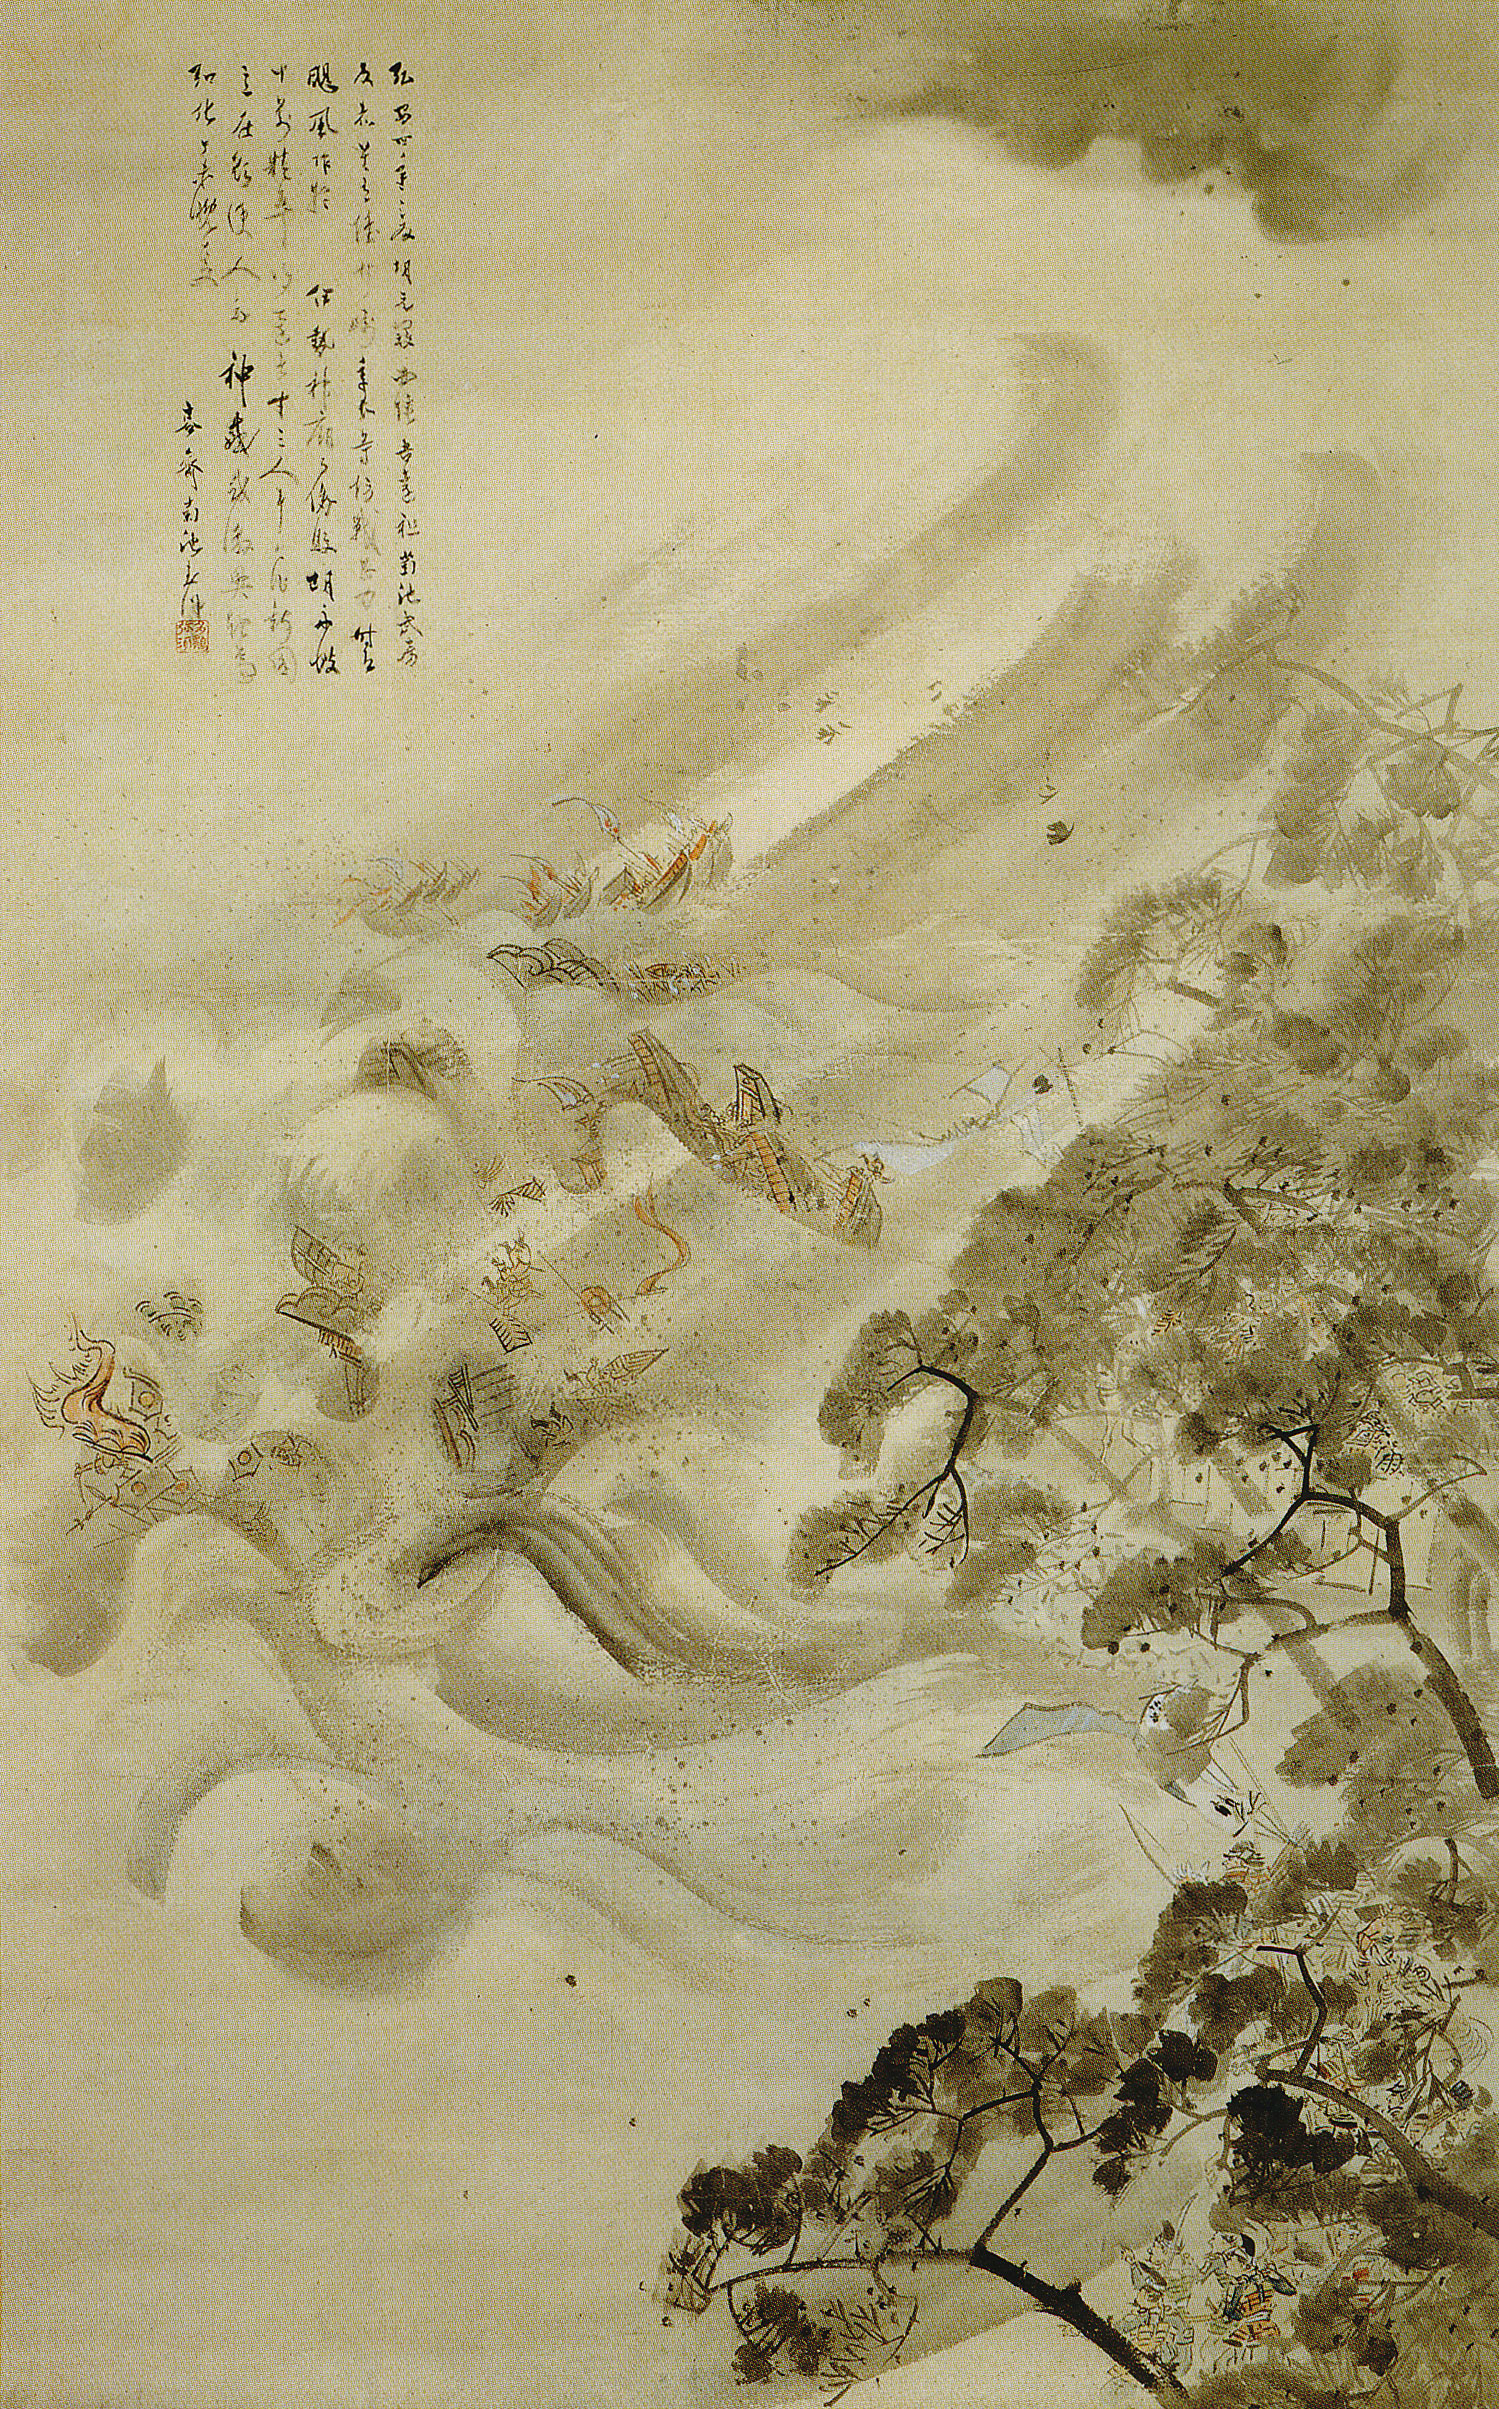
\includegraphics[width=0.38\textwidth]{MokoShurai.jpg}
    \caption{\small The Mongol fleet destroyed in a typhoon, ink and water on paper, by Kikuchi Y\={o}sai, 1847. 
    Source: Wikipedia}
    \label{fig:mongolJapan}
\end{wrapfigure}

\emph{Earth}, \emph{Wind}, \emph{Fire} \& \emph{Water}, the \emph{classical elements} were the basis 
for understanding our environment during antiquity. Modern science, based on experiments has taken a very 
different view of the world, one based on atoms, fundamental particles and states of matter. But we could 
argue that the classical elements were a more a philosophical idea that distilled our everyday experiences 
with nature, infact many ancient cultures such as Hellenistic Greece, Babylonia, Japan, Tibet, China and 
India had similar lists of four or five elements. These civilizations had very different views on the 
properties of these elements and how they related to natural phenomena, quite often these links 
were mythological. Indeed the obvious way in which people experienced the classical elements was through
weather systems. 

From the seasons to daily variations, nature's elements drive and shape our lives. Sometimes weather 
has had a direct impact on entire populations, one example was the failed Mongol invasions of Japan 
in $1274$ and $1281$. In both attacks, the Mongol fleets were almost entirely destroyed by storms called 
\emph{kamikaze} (translates to divine wind). Although some attacking Mongol forces did manage to land during 
the $1274$ campaign and outnumbered the defending armies, they were still defeated by Samurai clans with 
superior knowledge of the terrain. 

The invading fleet of $1281$ was composed of "more than four thousand ships bearing nearly $140,000$ men" 
\citep[pg.~17]{mcclain2002japan}, the scale of which was eclipsed only by the allied invasion of Normandy 
in 1944. The fleet was a hastily assembled, consisting of ships which were not suitable for the harsh waters 
between Japan and Korea. The Japanese had built two metre high walls in the intervening period and the invading 
fleets were forced to stay in sea for months. After their supplies were diminished, powerful kamikaze winds 
destroyed them entirely (an artists' view of the event is in figure \ref{fig:mongolJapan}). The failed invasions 
were a blow to the idea of Mongol supremacy in Asia and the Mongols never attemped an invasion of Japan since.

We now know that weather phenomena are caused by a combination of air pressure, temperature and moisture differences 
between one place and another. The angle of the Sun's rays changes with latitude, these variations create very 
different temperature trends from the poles to the equator. These differences in temperature lead to large scale 
air currents which create complex weather systems and climate patterns which we see across the world.

But weather phenomena are hardly exclusive to planet Earth.

\section*{The Final Frontier}

\begin{wrapfigure}{r}{0.4\textwidth}
    \centering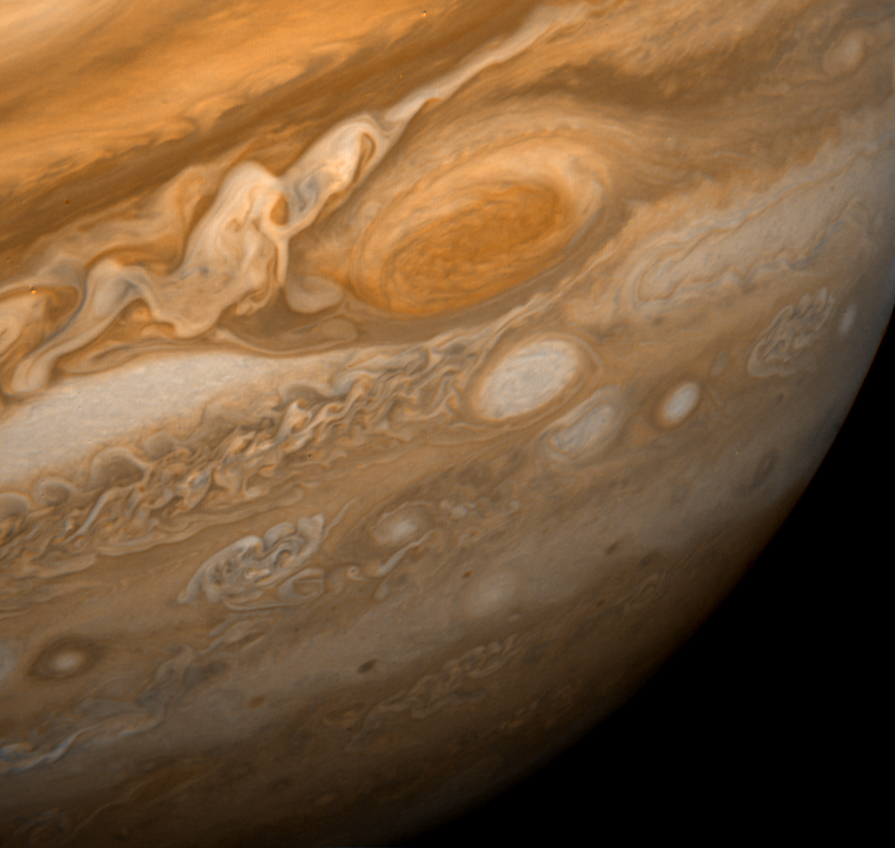
\includegraphics[width=0.38\textwidth]{Great_Red_Spot_From_Voyager_1.jpg}
    \caption{
        \small Jupiter's Great Red Spot in February 1979, photographed by the unmanned Voyager 1 NASA space probe. 
        Source: Wikipedia
    }
    \label{fig:jupiter}
\end{wrapfigure}

Even before the beginning of the space age, weather phenomena occurring on other planets have been observed. Jupiter's 
\emph{great red spot}, a huge storm, has been continuously observed since 1830 \citetext{see \citealp{britannicaRedSpot}}.
Saturn's \emph{great white spot}, a recurring storm system which was first used by Asaph Hall to determine the period of
the planet's rotation \citep{wikisaturn}. In the $20^{\text{th}}$ century, missions such as the Hubble space telescope, 
Voyager, Cassini and others have shown storms and other weather phenomena on planetary bodies like Venus, Mars, 
Neptune and Titan. 

The principles behind many planetary weather phenomena are very similar, their differences are because of the different 
compisition of each planet's atmosphere. Extra-terrestrial weather is just as complex and mind boggling as weather we 
observe on Earth, its scale is certainly much larger than we are used to. 

Yet, planetary weather is just one side of the puzzle. Venturing into our cosmic neighbourhood, our solar system
has another kind of weather system that has begun to be probed only very recently. 

\subsection*{A Gust of Wind from the Heavens}

During the last week of August 1859, several spots appeared on the surface of the Sun. Southern auroral displays were 
observed on August 29, as far north as Queensland Australia. Just before noon on September 1, British astronomer 
Richard Carrington observed a "white light flare" from a group of sun spots. He created a sketch of his observations
which is seen in figure \ref{fig:carringtonevent}. Carrington's observations were independently verified by British 
publisher and astronomer Richard Hodgson, both of them sent their reports to the 
\emph{Monthly Notices of the Royal Astronomical Society}.

September 1-2 1859 saw some remarkable events occur around the world. Auroral displays were observed all around the 
world, even in low latitude places such as Colombia \citep{MORENOCARDENAS2016257}. Auroras above the rocky mountains
in the U.S were so bright that they woke up gold miners who began preparing breakfast thinking it was morning 
\citep{miners}. In the northeastern U.S, people could read the newspaper by the aurora's light \citep{auroraReading}.

\begin{wrapfigure}{l}{0.4\textwidth}
    \centering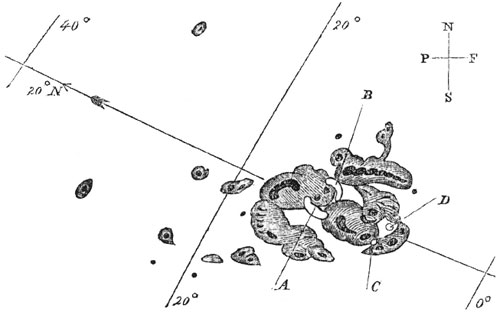
\includegraphics[width=0.38\textwidth]{Carrington_Richard_sunspots_1859.jpg}
    \caption{\small Sunspots of September 1, 1859, as sketched by Richard Carrington. 
    A and B mark the initial positions of an intensely bright event, 
    which moved over the course of five minutes to C and D before 
    disappearing. Source: Wikipedia}
    \label{fig:carringtonevent}
\end{wrapfigure}

The telegraph network in Europe and North America failed. Some operators experienced electric shocks 
\citep[pg.~13]{board2008committee} while in some cases even telegraph equipment that was disconnected 
from the power supply could be used to transmit messages \citep[pg.~58]{carlowicz2002storms}.

Based on global reports and observations taken by Scottish physicist Balfour Stewart at the 
Kew observatory in London, Carrington was able to connect events observed on the Earth to what 
he saw on the Sun on the $1^{\text{st}}$ of September \citep{clark2007sun}. His assertion was corraborated
by other observers in the scientific community.

The storm of 1859, later known as the \emph{Carrington event} was in some ways the genesis of \emph{Space Weather},
although the actual term was coined much later in the $1950$s. Although scientists had observed sunspots and their 
links to magnetic field variations on the Earth earlier, the \emph{Carrington event} was a concrete example of how 
activity on the Sun could have potentially dramatic effects on the Earth.

\subsection*{Space Weather}

\begin{wrapfigure}{r}{0.4\textwidth}
    \centering\includegraphics[width=0.38\textwidth]{induction_experiment.png}
    \caption{
        \small One of Faraday's 1831 experiments demonstrating induction. 
        The liquid battery (right) sends an electric current through the small coil (A). 
        When it is moved in or out of the large coil (B), its magnetic field induces a momentary 
        voltage in the coil, which is detected by the galvanometer (G). 
        Source: Wikipedia}
    \label{fig:induction}
\end{wrapfigure}

How do spots and ejections from the Sun produce bright lights and currents on Earth? During Carrington's time 
the fledgling science of Electromagnetism had picked up in the $19^{\text{th}}$ century and  already had some 
understanding of these phenomena. Faraday's induction experiment from 1831 (figure \ref{fig:induction}) had shown 
that varying magnetic fields could induce electrical currents in copper wires.

It took approximately a century from the \emph{Carrington event} for a theoretical understanding of Space 
Weather phenomena to develop. Maxwells equations of Electromagnetism \citep{maxwell1865viii} published in 
$1864$ gave scientists the mathematical tools to model the motions charged particles in electric and 
magnetic fields and the variations in the fields themselves due to those moving particles.

The $20^{\text{th}}$ century saw rapid progress made in modelling of charged particles in the Earth's magnetic 
field in the area of \emph{plasma physics}. Plasma was the name given to the state of matter containing 
positive and negatively charged particles in roughly equal numbers. Space weather started gaining relevance 
with the rise of space missions and satellites, though there was still much progress to be made. This was 
especially important with increasing reliance on electronic appliances and communication networks.

The Quebec power grid failure of 1989 \citep{kappenman1997geomagnetic} during a geomagnetic storm event showed 
that intense space weather events like the one observed in 1859 could cause significant damage to communications, 
energy and technological infrastructure that so crucial to the functioning of modern civilization.

But the solar storms observed in the $20^{\text{th}}$ and $19^{\text{th}}$ centuries are only one part of the 
picture. It is now increasingly likely that private companies will be making significant inroads into space 
travel for business goals. Companies such as SpaceX and BlueOrigin aim to make space travel cheaper and more 
accessible so that human beings can live and work in space or other planets in the solar system, potentially 
starting a second space age.


\begin{wrapfigure}{l}{0.4\textwidth}
    \centering\includegraphics[width=0.38\textwidth]{spacex.jpg}
    \caption{
        \small Artist's impression of the Interplanetary Starship on the Jupiter's moon Europa Source: Wikipedia}
    \label{fig:spacex}
\end{wrapfigure}

This drastic move to become a multi-planetary species will bring with it the risks to the human life and equipment. 
These risks come in the form of severe magnetic storms, solar flares and ejections of charged particles, which must 
be anticipated if we want to become a succesful space faring race. 

\subsection*{Space Science Informatics}

In order to design resilient technological systems for the new space age, we need to make progress in understanding 
and anticipating space weather phenomena. Physical theories about space plasmas needed to be combined with the data 
collected from space missions. The rapid rise of hardware, software, data storage, the deluge of space mission data 
and the advent of machine learning techniques means that we are in a unique position to take strides towards our 
space goals.

This thesis aims to be an exploration into the possibilities of space science informatics. It is structured as follows.



\clearpage
\bibliographystyle{plainnat}
\bibliography{references}


\clearemptydoublepage

\chapter{Preliminaries}\label{chapter:preliminaries}
\chapter{Preliminaries}\label{chapter:preliminaries}

\emph{Space weather} is the branch of physics that studies the time varying phenomena in the solar 
system. The principal driver of space weather phenomena is the Sun, specifically its magnetic field 
variations and the \emph{solar wind}. The effect of solar variations on the planetary environment 
are caused by the coupling between solar wind particles and the magnetic field produced by the 
Earth. This chapter gives a semi-quantitative treatment of various scientific ideas relevant to 
space weather research.

\begin{table}
    \centering
    \begin{tabular}{l p{0.35\textwidth} r}
        \hline
        \textbf{Chapters} & \textbf{Themes} & \textbf{Recommended Reading}\\
        \hline
        \vspace{5pt}
        \ref{chapter:dst_osa} \& \ref{chapter:dst_msa} & Forecasting of geomagnetic index $\mathrm{Dst}$. & \S~\ref{sec:geoindex}, \S~\ref{sec:mag}\textsuperscript{*}, \S~\ref{sec:plasma}\textsuperscript{*} \\
        \ref{chapter:bayes_diff_chapter} & Inference of radiation belt parameters. & \S~\ref{sec:plasmadiff}, \S~\ref{sec:plasma}\textsuperscript{*} \S~\ref{sec:mag}\textsuperscript{*} \\
        \ref{chapter:pdt} & Forecasting of near Earth solar wind speed using solar data. & \S~\ref{sec:hmfsolarwind}, \S~\ref{sec:sunspots}, \S~\ref{sec:solar}\textsuperscript{*}\\
        \hline
    \end{tabular}
    \caption{Dissertation Guide. {\small Asterisk\textsuperscript{*} denotes optional material.}}
    \label{table:chapterguide}
\end{table}

\Cref{table:chapterguide} provides the reader with a condensed guide to this dissertation. 
It connects the content presented in this chapter with the main research problems analyzed in the 
later chapters and provides recommended prerequisite reading for each chapter.

\Cref{sec:plasma} describes space plasmas and their properties. \Cref{sec:solar} provides some 
background about the Sun and the solar wind which is the driver for all space weather phenomena. 
This is used in the solar wind prediction task considered in \cref{chapter:pdt}. 
\Cref{sec:plasmadiff} introduces the plasma diffusion model (\cref{eq:fokker}) and its simplified 
radial diffusion system (\cref{eq:radialDiff}) which is used as the underlying physical model for 
\cref{chapter:bayes_diff_chapter}. \Cref{sec:mag} introduces the \emph{magnetosphere}, giving 
context for \cref{chapter:dst_osa,chapter:dst_msa}. 


\section{Space Plasma}\label{sec:plasma}

Plasma, also known as the fourth state of matter due to its properties that differentiate it 
from the conventional gaseous state, is ubiquitous throughout the visible Universe. Plasma is a gas 
which is composed of roughly equal number of positive and negatively charged particles, a property 
known as charge \emph{quasi-neutrality}. The term quasi-neutral is used because although the gas 
has almost equal amounts of positive and negative charges, the mixture is electromagnetically 
active. Due to incomplete charge shielding, long range electromagnetic fields play a big role in 
the dynamics of plasma.

%From classical electrostatics the electric potential of a point charge $q$, is given as

%\begin{equation}
%    \phi(r) = \frac{q}{4\pi\epsilon_0 ||r||_2}
%\end{equation}

%where $r$ is the position in space with respect to the charge and $\epsilon_0$ is the \emph{permittivity} of vacuum.

\subsection*{Debye Length}

In a quasi-neutral plasma, due to the presence of partial electric shielding the potential due to 
the charges now takes the well known Debye form
%
\begin{equation}
    \phi(r) = \frac{q}{4\pi\epsilon_0 r} e^{-\frac{r}{\lambda_d}} \ , 
\end{equation} 
%
where $r$ is the spatial distance with respect to the charge and $\epsilon_0$ is the 
\emph{permittivity} of vacuum. The electric potential decays with the Debye length scale 
$\lambda_d$ at which a balance between thermal vibrations which can disturb quasi-neutrality, and 
electrostatic forces due to charge separation, is achieved. The Debye length scale depends on the 
electron temperature and plasma density.
%
\begin{equation}\label{eq:debye}
    \lambda_d = \sqrt{\frac{\epsilon_0 k_b T_e}{n_e e^2}}
\end{equation}
%
In \cref{eq:debye} above, the Debye length scale is expressed in terms of the 
\emph{Boltzmann constant} $k_b$, the electron temperature $T_e$, free space permittivity 
$\epsilon_0$, and electron charge $e$. One can visualise the positively charged ions having a cloud 
of electrons shielding them at the distance of $\lambda_d$. 

It is also possible to take into account the shielding effect of the ions. The effective Debye 
length is now expressed as an addition of two terms: one for electrons (\cref{eq:debye}) and a 
similar term for the ions by replacing $T_e$ for the ion temperature $T_i$ ($n_i \approx n_e$). 

\subsection*{Plasma Parameter}

Consider a Debye sphere of radius $\lambda_d$. This sphere contains 
$N_e = \frac{4}{3}\pi \lambda^3_d n_e$ electrons. The plasma parameter $g$ is defined as 
$N_{e}^{-1}$. Rewriting this, we can say:
%
\[
    g \sim \sqrt{\frac{n_e}{T_e}} \ .
\]
%
The description of plasma used in many applications in space is applicable when $g \ll 1$. In 
this situation the Debye shielding is significant, and the quasi-neutral plasma obeys collective 
statistical behavior. The plasma parameter $g$ also correlates with the collision frequency. The 
collisions in plasma increase with increasing density and decreasing temperature, and if 
$g \longrightarrow 0$ the plasma becomes nearly collisionless. The collisionless property helps in 
making simplifying assumptions about plasma dynamics and serves as the starting point for the 
\emph{adiabatic} theory of plasma motions in the Earth's magnetosphere which will be discussed in 
\cref{sec:plasmadiff}.

\section{Sun \& the Solar Wind}\label{sec:solar}

\begin{figure}
    \noindent\centering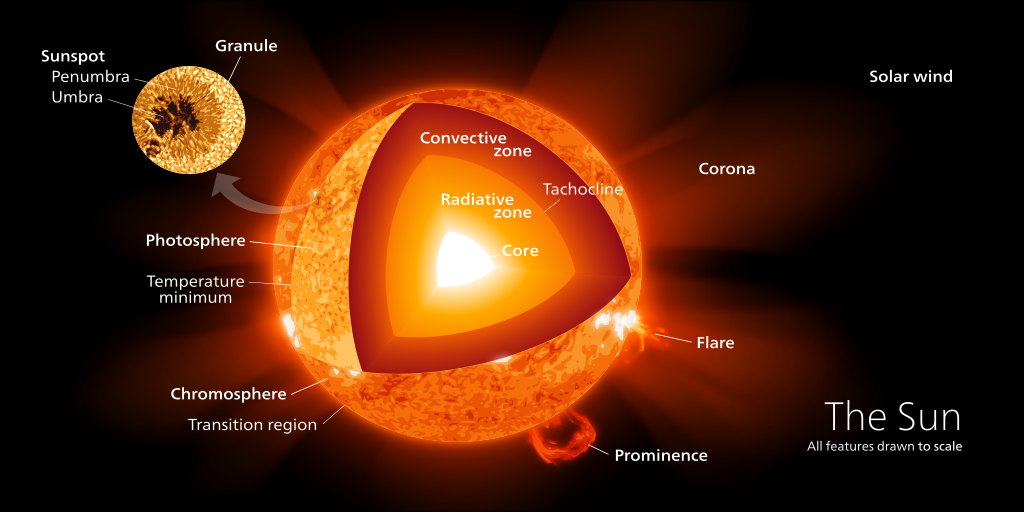
\includegraphics[width=\textwidth]{Sun_poster.png}
    \caption{{\small Cross section of the Sun \\ 
    Author: Kelvinsong [CC BY-SA 3.0 (\url{https://creativecommons.org/licenses/by-sa/3.0})]}}
    \label{fig:SunLayers}
\end{figure}

The Sun is an almost perfectly spherical ball of plasma which is the the center of our solar 
system and the only source of light and energy for all living and meteorological processes on 
Earth. Apart from terrestrial weather, the Sun is also the primary driver of space weather which 
results from the interaction between the solar wind and planetary magnetospheres.

\subsection{Structure}

\Cref{fig:SunLayers} shows a cross section of the Sun with various layers. We give a brief 
description of them below.

\textbf{Core}: The core of the Sun is the site for the thermonuclear fusion reactions which produce 
its energy. It extends from the center to about $20-25\%$ of the solar radius \citep{SolarAct}. It 
has a temperature close to $\SI{1.57d7}{\kelvin}$ and a density of 
$\SI{150}{\gram\per\centi\metre^3}$ \citep{SolarCore}. Nuclear fusion in the core takes place via 
the well known \emph{proton-proton chain} (pp).

\textbf{Radiative Zone}: The radiative zone extends from $25\%$ to $70\%$ of the solar radius. 
The nuclear reactions in the core are highly sensitive to temperature and pressure. In fact, they 
are almost shut off at the edge of the core. In the radiative zone, energy transfer takes place via 
photons (radiation) which bounce around nuclei until they reach the convective zone.

\textbf{Convective Zone}: The convective zone lies between $70\%$ of the solar radius to a point 
close to the solar surface. Density decreases dramatically going from the core to the radiative 
zone and subsequently the convective zone. In this region, the solar material behaves more like a 
fluid. Due to the temperature gradient which exists across it, the primary source of transport is 
here via convection.

\textbf{Photosphere}: The photosphere is the visible \enquote{surface} of the Sun, since the layers 
below it are all opaque to visible light. A layer of about $\SI{100}{\kilo\metre}$ thickness, the 
photosphere is also the region from where sunlight can freely escape into space. The photospheric 
surface has a number of features i.e. sunspots, granules and faculae. Sunspots 
(see \cref{sec:sunspots}) are magnetic regions where the solar material has a lower temperature 
compared to its surroundings. Magnetic field lines are concentrated in sunspot regions, and the 
field strength in sunspots can often be thousands of times stronger than the on the Earth.

% \begin{wrapfigure}{r}{0.4\textwidth}
%     \centering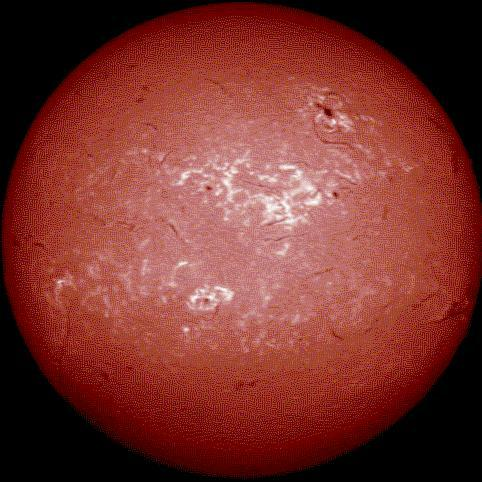
\includegraphics[width=0.38\textwidth]{chromosphere.jpg}
%     \caption{
%         {\small Chromosphere viewed using an $H\alpha$ filter. \\ \textit{Source}: CWitte (Public domain)}}
%     \label{fig:chromosphere}
% \end{wrapfigure}

\begin{wrapfigure}{r}{0.4\textwidth}
    \centering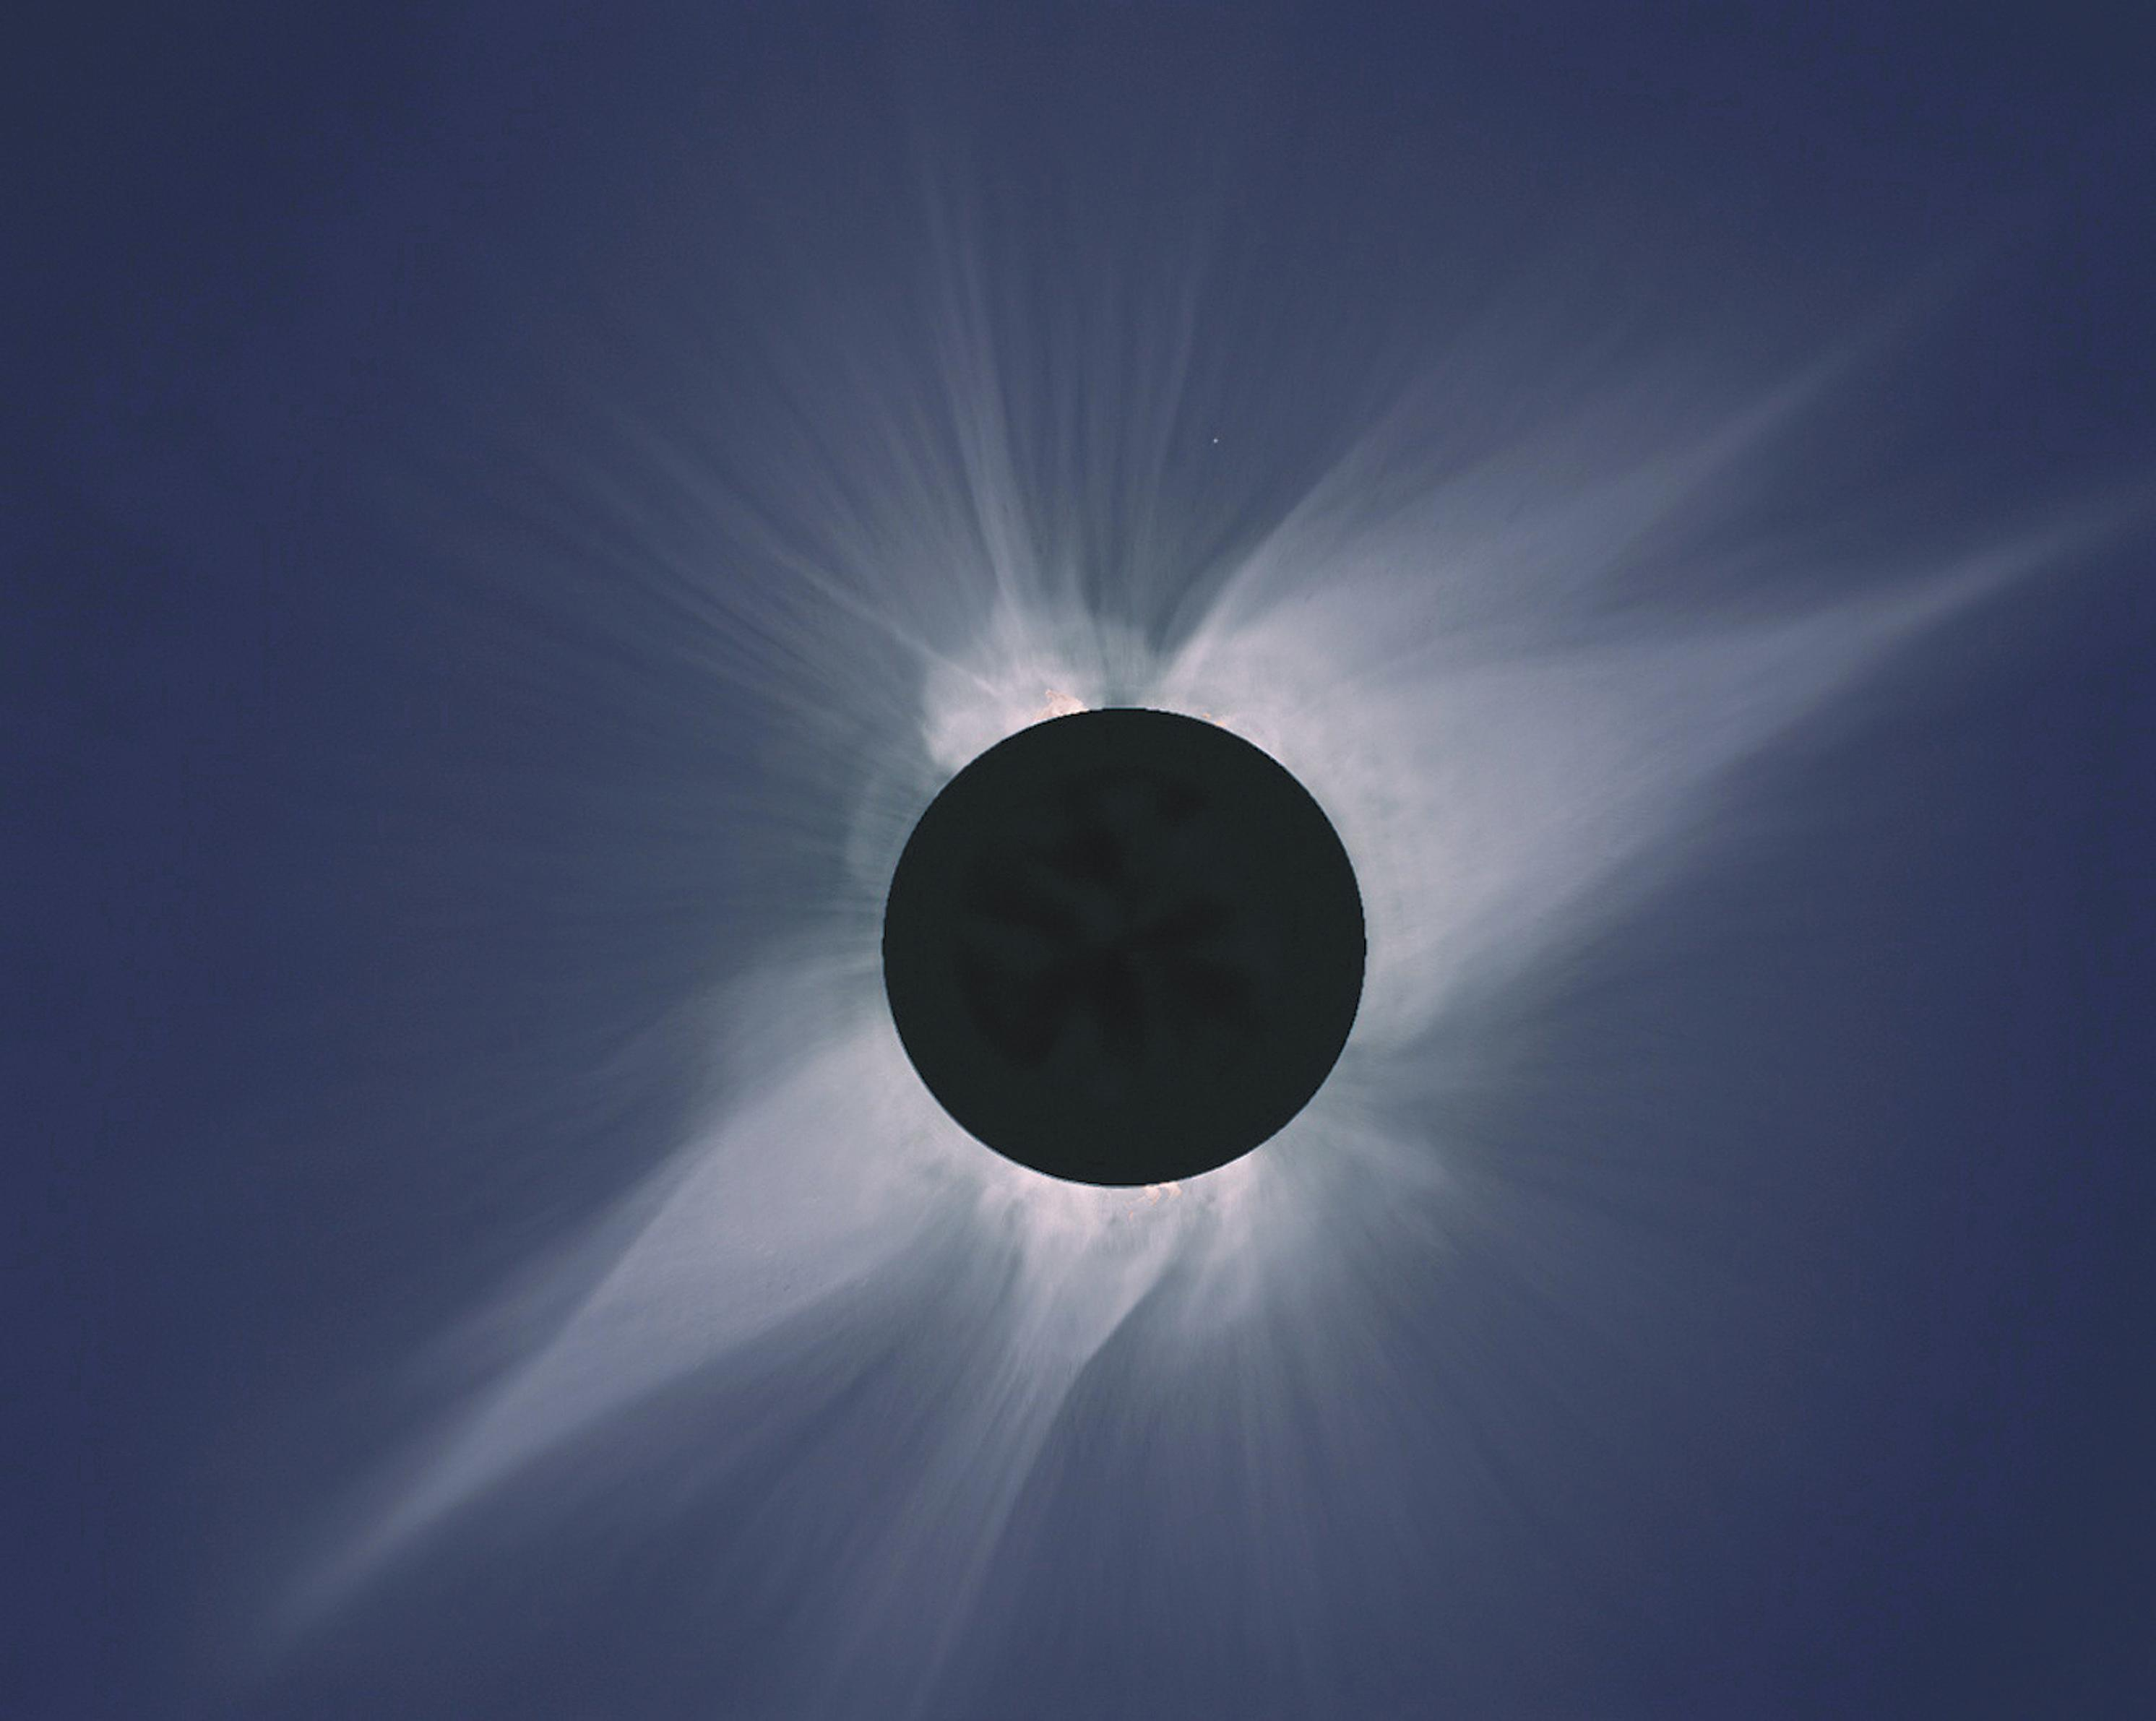
\includegraphics[width=0.38\textwidth]{coronaBaja.jpg}
    \caption{
        {\small 
            Sun's corona captured during a solar eclipse. \\ 
            \textit{Source}: Steve Albers, Boulder, CO; Dennis DiCicco, Sky and Telescope; 
            Gary Emerson, E. E. Barnard Observatory
        }
    }
    \label{fig:coronaBaja}
\end{wrapfigure}


\textbf{Chromosphere}: The Chromosphere extends for a distance of almost $\SI{5000}{\kilo\metre}$ 
after the photosphere. The chromosphere is known for the existence of features called spicules and 
prominences. The chromosphere has a red colour which is generally not visible due to the intense 
light given off by the photosphere but can be observed through a filter centered on the Hydrogen 
$H\alpha$ spectral line. %(see figure \ref{fig:chromosphere}). 

\textbf{Solar Transition Region}: A thin ($\SI{100}{\kilo\metre}$) region between the chromosphere 
and the solar corona where the temperature rises from about \SIrange{8000}{5d5}{\kelvin}, the solar 
transition region might not be well defined at all altitudes; however its existence is evidenced by 
a bifurcation of the dynamics of the solar plasma. Below the transition region, the dynamics is 
dictated by gas pressure, fluid dynamics, and gravitation while above the region, the dynamics is 
dictated more by magnetic forces.

\textbf{Corona}: An aura of plasma around the Sun that extends millions of kilometers into space, 
the corona can be observed during a total solar eclipse (\cref{fig:coronaBaja}) or with a 
coronagraph. The temperature of the corona is dramatically higher than the photosphere and 
chromosphere. The average temperature can range from \SIrange{1d6}{2d6}{\kelvin} while in the 
hottest regions it can be as high as $\SI{2d7}{\kelvin}$ \citep{SolarCorona}. Although the reason 
for this dramatic increase is still not well understood, there exist various explanations using 
concepts of magnetic reconnection \citep{russell2001solar,SolarCorona} and Alfv\'en waves 
\citep{AlfvenCorona}. There is a critical height in the corona, known as the \emph{source surface}, 
below which the magnetic field controls the plasma completely. Above it the plasma carries 
the magnetic field with it into the interplanetary medium.


\subsection{Solar Wind \& Heliospheric Magnetic Field}\label{sec:hmfsolarwind}

The idea that the Sun was ejecting charged particles outwards into space was first hinted at after 
the solar storm of $1859$ by Richard Carrington \citep{cliver20131859} and later by George 
FitzGerald \citep{meyer2007basics}. Arthur Eddington, in a footnote of an article about the comet 
Morehouse in $1910$, was the first to suggest the existence of the solar wind, without naming it so 
\citep{eddingtonFootnote}.

In the $1950\text{s}$, studies of the anti-solar orientation of the ion tails of Halley's comet 
led to the theory of solar corpuscular emission \citep{Bierman1,Bierman2,Bierman3}. 
\citet{parker1958dynamics,Parker1960,Parker1965} argued that the corona cannot remain in 
hydrostatic equilibrium and that supersonic expansion of the corona is responsible for the 
outward expulsion of charged particles, which the author referred to as the \emph{solar wind}.

\citet{parker1958dynamics} also proposed a spiral model for the \emph{Heliospheric Magnetic Field} 
(HMF) and suggested that the solar wind carried with it the solar magnetic field. The Parker model 
was further supported its ability to explain the effect of the HMF on the modulation of galactic 
cosmic rays and their measured intensities close to the Earth \citep{ParkerSolarWind}. In $1959$ 
the Soviet spacecraft Luna $1$ was the first to directly observe the solar wind and measure its 
strength \citep{harvey2007russian}. Subsequently, the Mariner $2$ mission recorded properties of 
the positive ion component of the solar wind and confirmed the Parker spiral HMF model 
\citep{neugebauer1966mariner}.

The structure of the HMF is central to explaining the formation and propagation of the solar wind. 
The HMF in steady state points radially outward and rotates with the Sun, producing an 
\emph{Archimedean spiral} structure as postulated in \cite{parker1958dynamics} and shown 
schematically in \cref{fig:parkerspiral}. Photospheric observations of the magnetic field (see 
Global Oscillation Network Group \url{https://gong.nso.edu}) are often extrapolated to compute 
approximations to the coronal HMF topology. There exist a number of techniques used to perform such 
extrapolations: potential field based methods such as \emph{Potential-Field Source Surface} (PFSS) 
\citep{schatten1969model,altschuler1969magnetic}, PFSS variants such as 
\emph{Potential-Field Current Sheet} (PFCS) \citep{schatten1971current}, 
\emph{Current-Sheet Source Surface} (CSSS) \citep{csss}, and several others. Apart from potential 
based models, there exist more involved techniques based on Magnetohydrodynamics (MHD) such as 
\emph{Magnetohydrodynamics Around a Sphere} (MAS) \citep{linker1999magnetohydrodynamic}, 
ENLIL \citep{ODSTRCIL1996,ODSTRCIL1999a,ODSTRCIL1999b,ODSTRCIL2003,ODSTRCIL2004} and EUHFORIA 
\citep{pomoell2018euhforia}. 

The HMF can be seen as a combination of two components: the poloidal magnetic field and the 
toroidal magnetic field. The two fields often exchange energy between themselves over the course of 
several years in a cyclical phenomenon known as the \emph{solar cycle} 
(\cref{sec:sunspots}). Interested readers can read \citet{Owens2013} for an in-depth review on the 
phenomena that drive the HMF.

\begin{figure}
    \noindent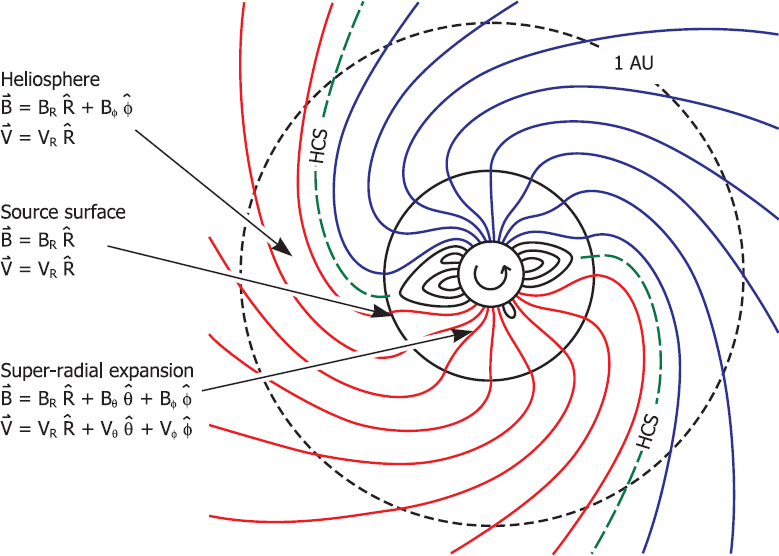
\includegraphics[width=0.8\textwidth]{parker-spiral.jpg}
    \caption{
        {\small 
            An illustration of the Heliospheric Magnetic Field in the \emph{ecliptic plane}. In the 
            heliosphere, rotation of the HMF foot points within a radial solar wind flow generates 
            an azimuthal component of the HMF, $B_{\phi}$, leading to a spiral geometry. Red and 
            blue lines, showing regions of opposite polarity, are separated by the heliospheric 
            current sheet (HCS), shown as the green dashed line. Image reproduced from 
            \citet{Owens2013}
        }
    }\label{fig:parkerspiral}
\end{figure}


The expansion of the coronal magnetic field leads to an eventual opening of field lines at the 
source surface (see \cref{fig:parkerspiral}) and the ejection of the solar wind. This hot plasma 
consists mostly of protons, electrons and a small number of helium and heavy ions. The solar wind 
spirals outwards in all directions, carrying with it the magnetic field. Close to the Earth's 
magnetosphere, this wind has a nominal speed of about $\SI{400}{\kilo\metre\per\second}$ while its 
high speed component has an average velocity of $\sim \SI{700}{\kilo\metre\per\second}$ 
(\cref{fig:solarwinddist}).

\begin{figure}
    \noindent\centering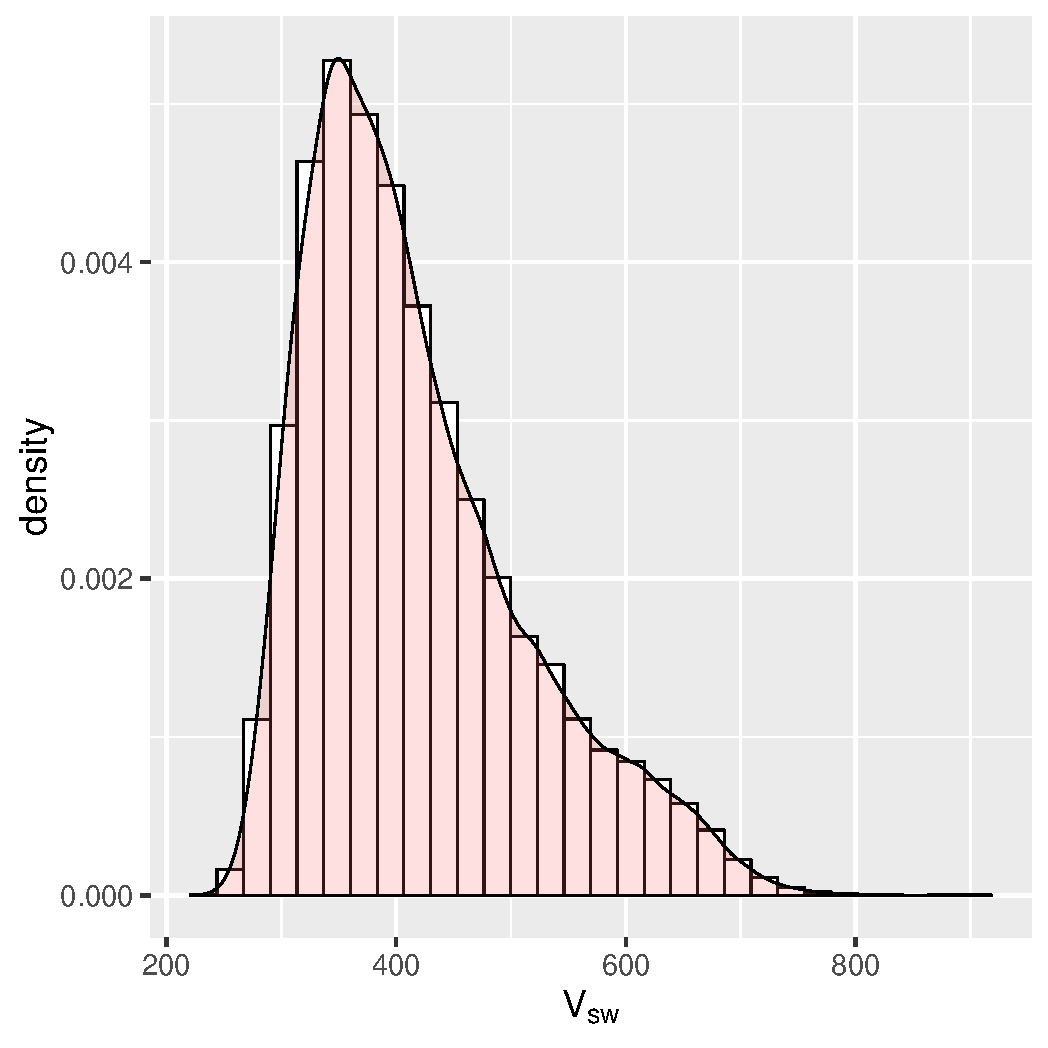
\includegraphics[width=0.75\textwidth]{solarwinddist.pdf}
    \caption{
        {\small 
            Distribution of solar wind speed recorded at $\SI{1}{\astronomicalunit}$ for the time 
            period $2008 - 2018$, \textit{Source}: OMNI data set 
            (\url{https://omniweb.gsfc.nasa.gov/ow.html})
        }
    }\label{fig:solarwinddist}
\end{figure}

\subsubsection*{Near Earth Measurements}

The solar wind has the heliospheric magnetic field \emph{frozen in} \footnote{the flux of the 
magnetic field going through a surface that moves with the solar wind (in a Lagrangian manner) is 
constant}, and as it propagates in the interplanetary medium, it carries the solar magnetic field 
with it \citep{alfven1942existence,alfven1943existence}. Important solar wind quantities such as: 
%
\begin{enumerate*} 
    \item solar wind speed, 
    \item proton density, and  
    \item magnetic field strength 
\end{enumerate*}
% 
are recorded at the well known $L1$ \emph{Lagrangian point} where the gravitational fields of the 
Earth and the Sun approximately balance out.



\subsection{Sunspots \& Solar Cycle}\label{sec:sunspots}

Sunspots are temporarily occurring regions on the Sun's photosphere that appear as dark spots. 
They are areas of magnetic field concentration where the field lines often \enquote{puncture} the 
solar surface inhibiting convection and producing regions with lower temperatures than the 
surroundings. Sunspots generally last anywhere between a few days to a few months. They can occur 
in pairs or groups and can accompany other phenomena such as \emph{coronal loops}, 
\emph{prominences}, and reconnection events.

Since the $19^{\text{th}}$ century the number of sunspots on the Sun's surface have been recorded 
as the \emph{sunspot number} (SSN). Sunspots populations increase and decrease, thereby behaving as 
markers for solar activity levels. The cyclical behavior of sunspot populations is called the 
\emph{sunspot cycle} or \emph{solar cycle} (\cref{fig:SolarCycle}). 

\begin{figure}
    \noindent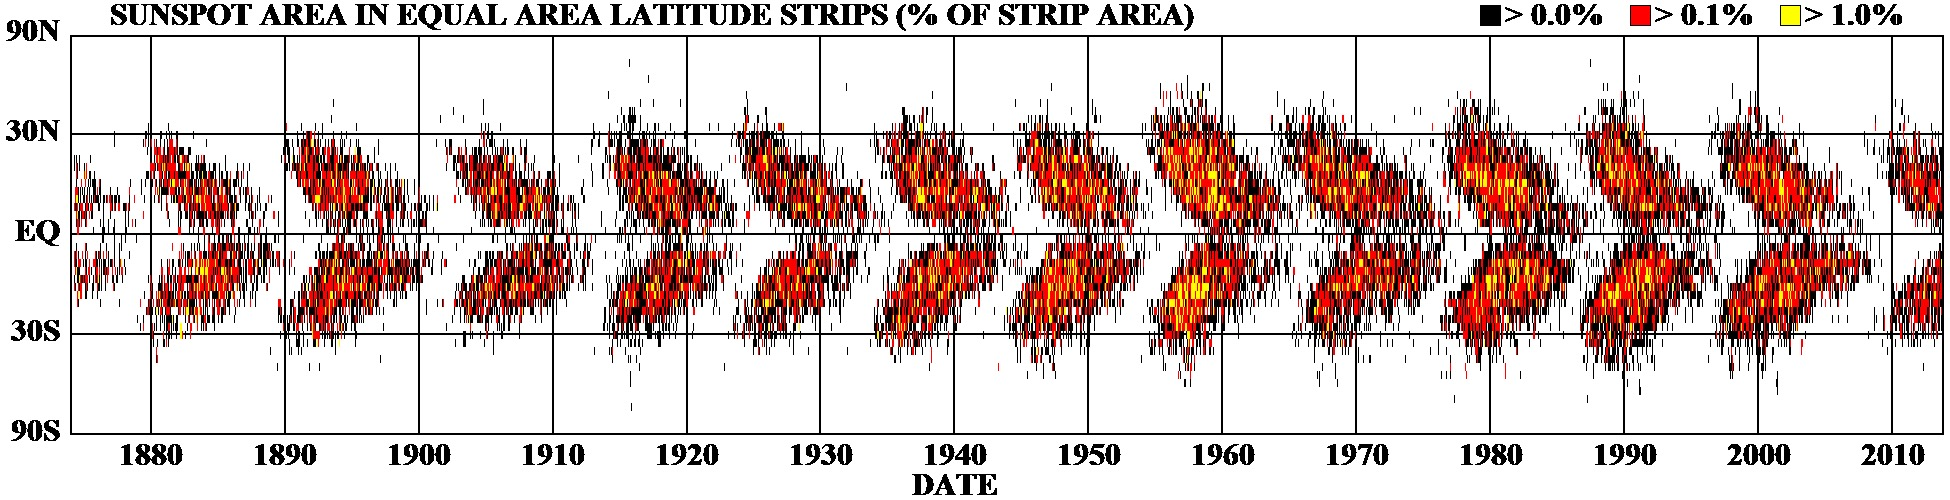
\includegraphics[width=\textwidth]{sunspot-cycle.jpeg}
    \caption{{\small The sunspot butterfly diagram.  \\ 
    \textit{Author}: David Hathaway, NASA, Marshall Space Flight Center (Public domain) \\ 
    \textit{Source}: Wikipedia}}
    \label{fig:SolarCycle}
\end{figure}

\Cref{fig:SolarCycle} depicts how the area occupied by sunspots changes with solar latitude 
and time. During the start of a solar cycle (solar minimum), sunspots start appearing at higher 
latitudes. Over the course of the cycle, they move towards the equatorial regions and their number 
increases to some maximum (solar maximum). Towards the end, the number of sunspots diminishes and 
the entire cycle starts over. This repetitive behavior happens over approximately $11$ years.

Because sunspots are magnetic phenomena, the solar cycle represents cyclical behavior of the HMF. 
During solar minimum, the poloidal component of the solar magnetic field is at its strongest and it 
is the closest it can get to a magnetic dipole configuration. Towards solar maximum, energy is 
transferred from the poloidal component to the toroidal component, resulting in complex field 
configurations which are evidenced by larger numbers of sunspot clusters.

The solar cycle also gives rise to variations in solar irradiance \citep{solarirradiance}. Between 
$1645$ and $1715$, very few sunspots were observed, a period known as the \emph{Maunder minimum}. 
This coincided with lower than average temperatures in Europe, which was called the 
\emph{little ice age}. Although the Maunder minimum was a period of lower solar irradiance, 
recent research \citep{owens2017maunder} has demonstrated that this was neither the only factor 
nor the most significant in causing lower than average temperatures during the little ice age.

In \cref{chapter:pdt}, the \emph{sunspot number} data as well as the \emph{flux tube expansion} 
factor ($f_S$ or FTE) and the magnetic field strength computed by the CSSS model will be used to 
create a input data set for building the \emph{dynamic time lag regression} model proposed therein. 
Using the input parameters, the \XX \ model provides an estimate for the near Earth solar wind 
speed as well as the propagation time. Measurements of the solar wind speed will also be used in 
\cref{chapter:dst_osa,chapter:dst_msa} as inputs to the Dst forecasting models applied therein.


\section{Magnetosphere}\label{sec:mag}

% \begin{figure}
%     \noindent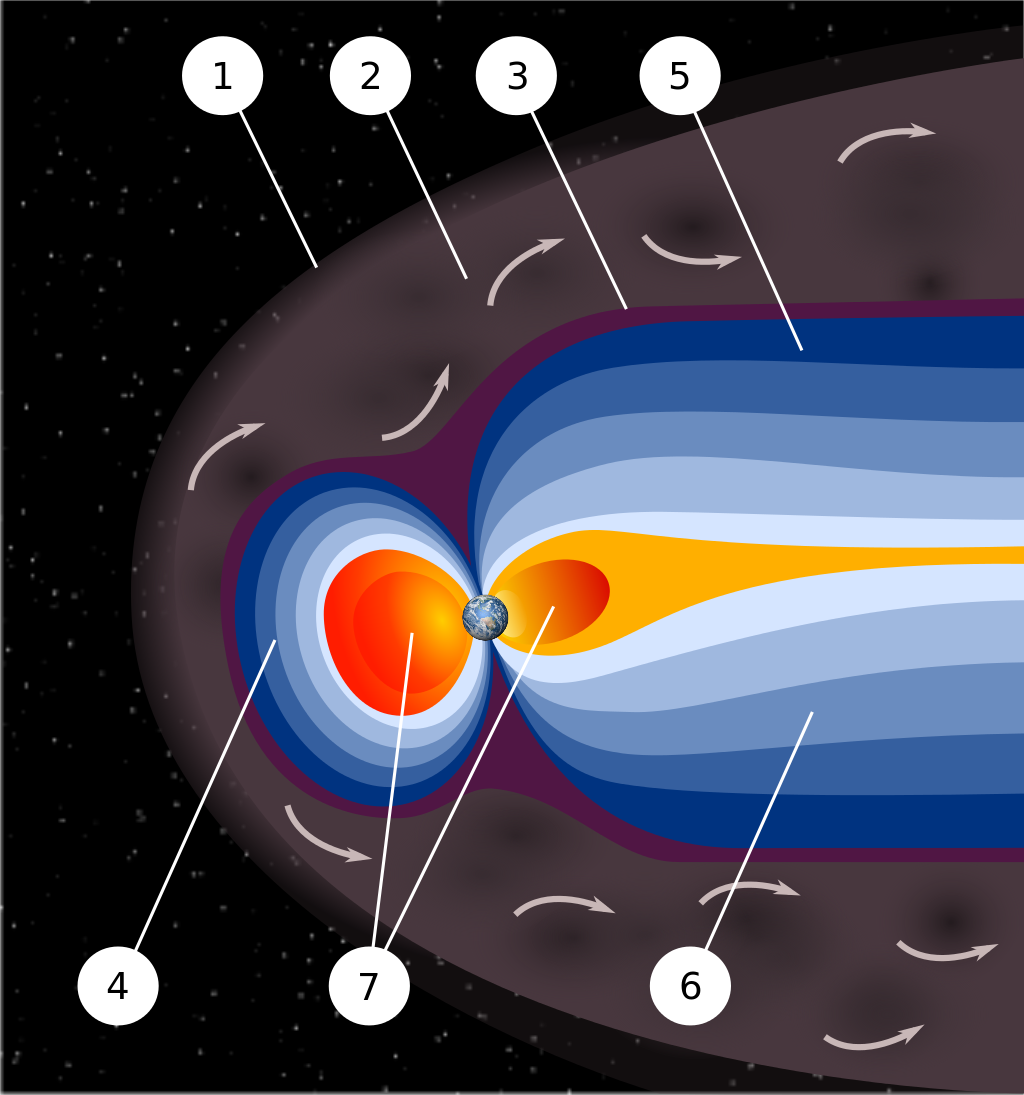
\includegraphics[width=0.7\textwidth]{mag.png}
%     \caption{{\small Schematic diagram of the Earth's magnetosphere: \\
%     The Sun (not shown) is to the left of the figure, the solar wind propagates from left to right.\\
%     1) Bow shock. 2) Magnetosheath. 3) Magnetopause. 4) Magnetosphere. \\
%     5) Northern tail lobe. 6) Southern tail lobe. 7) Plasmasphere.\\ 
%     Source: Dennis Gallagher, derivative work: Fr\'ed\'eric Michel (Public domain)}
%     }
%     \label{fig:magnetosphere}
% \end{figure}

\begin{figure}[ht]
    \noindent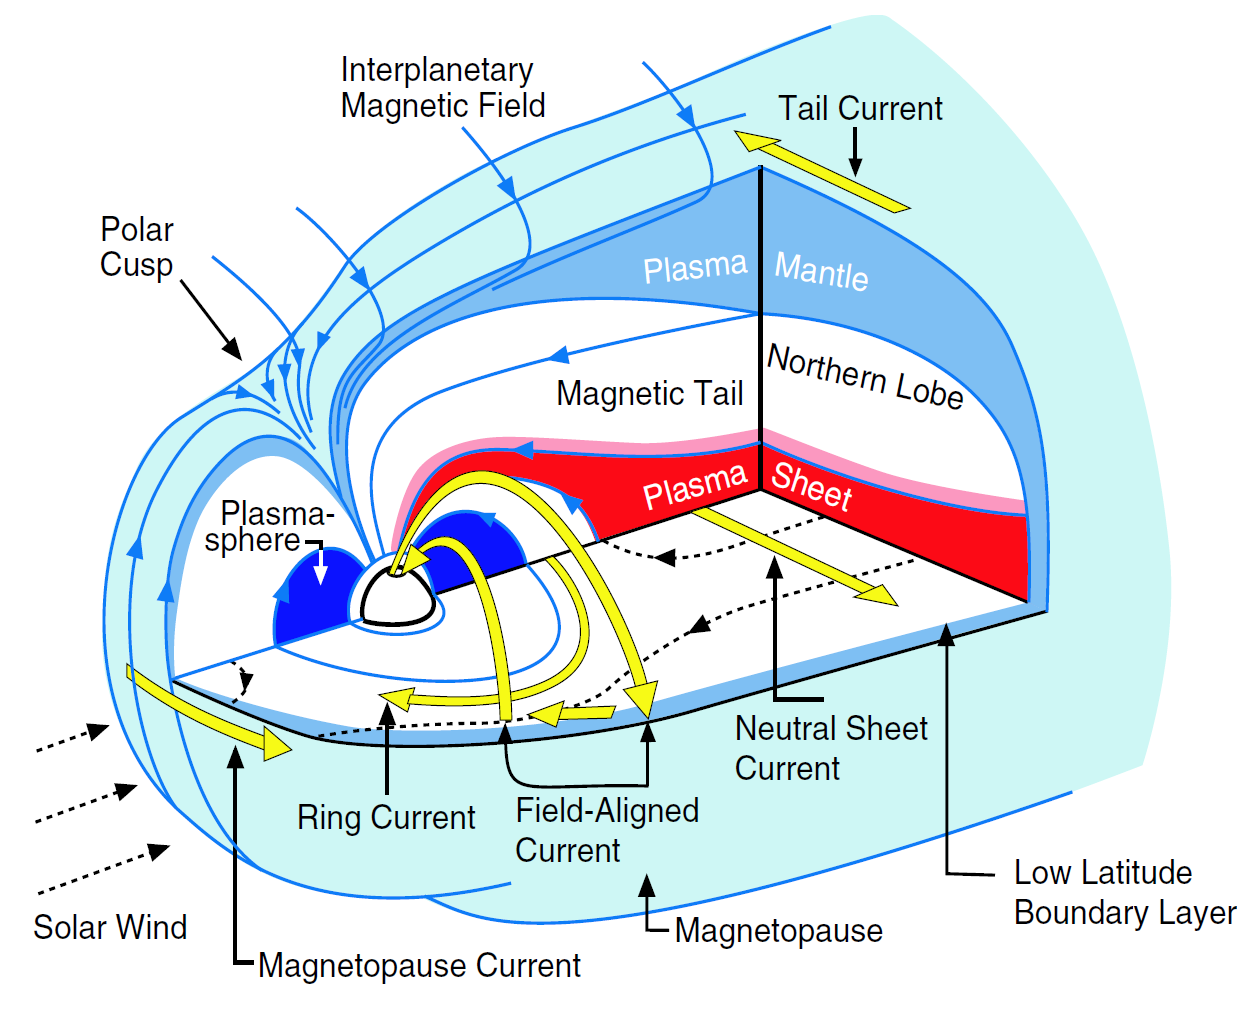
\includegraphics[width=0.8\textwidth]{mag3.png}
    \caption{
        {\small 
            Three-dimensional cutaway view of the magnetosphere. The light blue outer surface is 
            the magnetopause, and its boundary layers are shown in darker blue. Magnetic field lines 
            are shown in blue, electric currents in yellow. The polar region where the magnetic 
            field lines converge is the polar cusp. The bow shock has been omitted for clarity. 
            Image reproduced from \citet{DeKeyser2005}.
        }
    }
    \label{fig:magnetosphere}
\end{figure}

The Earth's magnetosphere (\cref{fig:magnetosphere}) is a region surrounding the planet where its 
magnetic field dominates the \emph{interplanetary magnetic field}. The Earth's magnetic field 
shields the atmosphere and terrestrial life from the impact of the solar wind. 

As the solar wind approaches the Earth, it is slowed down and deflected by the Earth's magnetic 
field. Since the solar wind is supersonic when it arrives and slows down to subsonic levels, a 
shock wave is generated in the process (\emph{bow shock}). Much of the solar wind kinetic energy is 
converted to thermal energy when it crosses the \emph{bow shock} into the \emph{magnetosheath}. The 
\emph{magnetosheath} spans from the \emph{bow shock} to the \emph{magnetopause}. The 
\emph{magnetopause} is the outer boundary of the Earth's magnetic shield. Its location is 
$\sim 10R_E$ ($R_E = \SI{6372}{\kilo\metre}$, the radius of the Earth). 


Earth's magnetic shielding is not perfect, and some particles manage to get trapped inside the 
cavity of the \emph{magnetosphere}. This region of trapped plasma is known as the the 
\emph{van Allen radiation belts}. Particles trapped in the radiation belts execute complex motions 
which can be approximately modelled using ideas from adiabatic theory and diffusion described in 
\cref{sec:plasmadiff} below. The \emph{plasmasphere} is the inner region of the radiation 
belts which contains cold, dense plasma. The portion of the magnetosphere facing away from the Sun 
(called the \emph{nightside}) is stretched out in a tail-like shape by the deflected solar wind, 
hence referred to as the \emph{magnetotail}. The \emph{magnetotail} has an approximate extent 
of up to $1000R_E$.


\subsection{Particle Motions \& Adiabatic Theory} \label{sec:plasmadiff}

This section gives a quick introduction to the theory of charged particle motions in the 
magnetosphere. The reader may refer to \citet{roederer2012dynamics} for an in depth treatment of 
this subject. To understand the motions of charged particles in the \emph{magnetosphere}, the role 
of electric and magnetic forces must be understood.

It is well known from classical electromagnetism that the force exerted on a particle with charge 
$q$ by a magnetic field $\mathbf{B}$ and an electric field $\mathbf{E}$ is given by the well known 
\emph{Lorentz force} (\cref{eq:lorentzforce}).
%
\begin{equation}\label{eq:lorentzforce}
    \mathbf{F} = m\frac{d\mathbf{v}}{dt} = q\mathbf{E} + q\mathbf{v} \times \mathbf{B}
\end{equation}
%
The first component of \cref{eq:lorentzforce} ($q\mathbf{E}$) is either parallel or opposite to the 
local electric field depending on the charge of the particle. The second component 
$q\mathbf{v} \times \mathbf{B}$ involves a vector cross product so it is always perpendicular to 
the plane spanned by vectors $\mathbf{v}$ and $\mathbf{B}$. In order to understand its effects, we 
can decompose the particle velocity in two components; $v_{\parallel}$ parallel to $\mathbf{B}$ and 
$v_{\perp}$ perpendicular to $\mathbf{B}$. If $\mathbf{E} = \mathbf{0}$, then the particle executes 
a circular motion with properties shown in \cref{eq:larmor}. Here $\rho$ is the gyroradius and 
$\omega$ is the gyrofrequency or cyclotron frequency. In the case where $v_{\parallel} \neq 0$, the 
trajectory is helical.
%
\begin{equation}\label{eq:larmor}
    \frac{v^{2}_{\perp}}{\rho} = \frac{qBv_{\perp}}{m} = \omega v_{\perp}
\end{equation}
%
Apart from the gyro motion, there are some important drift forces that significantly influence 
particle motions.
%
\begin{itemize}
    \item Electric field drift: If $\mathbf{E}$ has a component $E_{\perp}$ perpendicular to 
    $\mathbf{B}$, the electric field accelerates and decelerates the particle in the two 
    hemispheres of the orbit. The orbit becomes a distorted circle, and the particle drifts in a 
    direction perpendicular to the electric field with a velocity 
    $\mathbf{v_d} = \mathbf{E} \times \mathbf{B} / B^2$.

    \item Magnetic gradient drift: When the magnetic field varies in space (as is the case of the 
    Earth), a gradient in the field strength in the direction perpendicular to $\mathbf{B}$ gives 
    rise to a gradient drift velocity given by 
    $\mathbf{v_g} = \frac{1}{2} m v^2_{\perp}\mathbf{B} \times \frac{\nabla \mathbf{B}}{aB^3}$.

    \item Magnetic curvature drift: If the magnetic field has a curvature, this creates an 
    additional drift motion with velocity 
    $\mathbf{v_c} = \frac{ m v_{\parallel} \mathbf{B} \times (\hat{\mathbf{b}} \cdot \nabla) 
    \hat{\mathbf{b}} }{qB^2}, \ \ \mathbf{b} = \frac{\mathbf{B}}{B}$.
\end{itemize}

The equations of motion for charged particles in the general case of spatially varying electric and 
magnetic fields do not admit closed-form solutions. The motions are generally complex and require 
lengthy numerical integrations to be resolved.
%
\begin{figure}[ht]
    \centering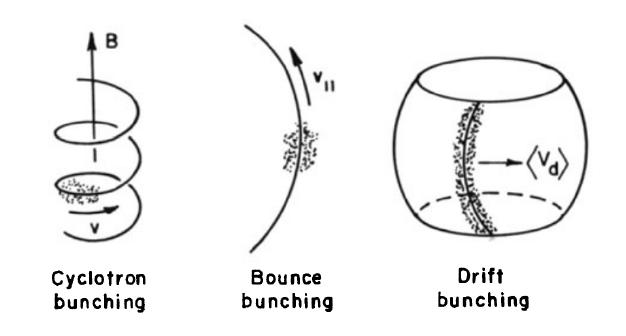
\includegraphics[width=0.4\textwidth]{adiabatic_motions.jpeg}
    \caption{
        {\small 
        The periodic components of the motion of trapped particles. Reproduced from 
        \citet{roederer2012dynamics}
        }
    }
    \label{fig:particlemotions}
\end{figure}
%
\todo{\textbf{TODO}: Check that the adiabatic motion image from Roederer can be reproduced here.}

The \emph{guiding center} approximation helps us to decompose particle motions into three periodic 
components (\cref{fig:particlemotions}):
%
\begin{enumerate*}
    \item gyration around magnetic field lines, 
    \item bounce motions between magnetic north and south poles, and
    \item equatorial drift of electrons and protons, 
\end{enumerate*}
%
each with its own time scale.

\subsubsection*{Adiabatic Invariants}

When a physical system with periodic motion is varied slowly as compared to the time period of 
its periodicity, the transformation can be characterized as \emph{adiabatic}. 
Formally speaking, for systems which are described by Hamiltonian dynamics, we can write the 
equations of motion in terms of the \emph{canonical position} $q$, the \emph{canonical momentum} 
$p$, external parameters $\theta$, and the system's \emph{Hamiltonian} $\mathcal{H}(q,p|\theta)$: 
%
\begin{equation}\label{eq:hamilton}
    \begin{aligned}
        \dot q &= \frac{\partial \mathcal{H}}{\partial p}\\
        \dot p &= - \frac{\partial \mathcal{H}}{\partial q} \ .
    \end{aligned}
\end{equation}
%
If the system shown in \cref{eq:hamilton} executes a periodic motion in the $q,p$ phase 
space, it admits an \emph{adiabatic invariant} $A$ given in \cref{eq:adiabatic_invariant}.
%
\begin{equation}\label{eq:adiabatic_invariant}
    A = \oint p d q
\end{equation}
%
The quantity $A$ would remain approximately constant if the external parameters $\theta$ were 
varied adiabatically (i.e. if changes in $\theta$ happen over a time period much greater than 
the period of oscillation of the system).

Applying the idea of adiabatic invariance to charged particle motion in the \emph{magnetosphere}, 
it is possible to associate one adiabatic invariant with each periodic motion i.e. gyromotion 
$\mathcal{M}$, bounce $J$, and drift $\Phi$ (\cref{eq:plasmainv}). 
%
\begin{align}\label{eq:plasmainv}
    \mathcal{M} &= \frac{1}{2}\frac{mv^{2}_{\perp}}{\rvert \mathbf{B} \rvert} \\
    J &= \oint{m_0 v_{\parallel}ds} \\
    \Phi &= \oint{v_{\text{drift}} \cdot r d\phi} = \int{\mathbf{B} d\mathbf{S}}
\end{align}
%
The first invariant $\mathcal{M}$ is associated with the Larmor gyration - it is the magnetic 
moment of the current generated by the circular motion of the particle around the field line. 

The second invariant $J$ is associated with the bounce motion between the two magnetic mirrors near 
the north and south poles (the quantity $s$ is an appropriately chosen arc length coordinate along 
the bounce trajectory). The bounce motion between the magnetic poles can be explained by the 
conservation of the particle energy $\frac{1}{2}m v^2_{\parallel} + \frac{1}{2}m v^{2}_{\perp}$ and 
the first invariant $\mathcal{M}$. Because field strength $\rvert \mathbf{B} \rvert$ increases 
near the poles, $v_{\perp}$ also increases to conserve $\mathcal{M}$; however, to conserve energy, 
$v_{\parallel}$ decreases until the particle can no longer move farther along the field line (and 
bounces back).

The third invariant $\Phi$, associated with equatorial drift motion, is actually the magnetic 
flux through the barrel shape envelope of the particle drift. A particle's guiding magnetic field 
line can be identified by its radial position $r$ and its longitude $\phi$. The magnetic flux of 
the drift can then be computed by integrating over $\phi$.

Associated with each adiabatic invariant is a timescale which determines how easily its 
conservation can be violated. The timescales for $\mathcal{M},\ J, \ \text{and} \ \Phi$ are the 
time periods of the gyromotion, bounce motion, and equatorial drift motion respectively. Since 
it takes much a longer time for the particles to complete a drift motion around the Earth as 
compared to bounce and gyromotion (in that order), the invariance of $\Phi$ is most easily 
violated - a fact which is used in the simplification of the Fokker-Planck diffusion system 
described below.    

\subsubsection*{Plasma Diffusion}

Because we consider populations of charged particles, it is natural to employ some kind of 
distribution based picture for magnetospheric plasma. The adiabatic invariants give us a phase 
space or coordinate system by which we can express quantities of interest. 

The main quantity of interest in this case is the \emph{phase space density} 
$f(t, \mathcal{M}, J, \Phi)$ which is a function of time and three invariants. The 
\emph{phase space density} tells us the number of particles in a particular region of the phase 
space, and at a particular point of time.

Diffusion behavior arises when one or more of the invariants are violated, which can happen due to 
a number of reasons such as: 
%
\begin{enumerate*}
    \item non-adiabatic variations of the magnetic field, 
    \item external forces, 
    \item interaction with electromagnetic waves, and 
    \item collisions with atmosphere/ionosphere. 
\end{enumerate*}
%
The plasma diffusion system \citep{schulz2012particle} can be written as a generalized 
Fokker-Planck system as shown in \cref{eq:fokker}.
%
\begin{align}\label{eq:fokker}
    \frac{\partial{f}}{\partial{t}} &= \sum^{3}_{p,q = 1}
    \frac{\partial}{\partial{J_{p}}} \left( \kappa_{pq}
    \frac{\partial{f}}{\partial{J_{q}}} \right) \\
    J_1 &= \mathcal{M} \\
    J_2 &= J \\
    J_{3} &= \Phi
\end{align}
%
It is possible to simplify this system by considering the two main categories of diffusion: radial 
diffusion and pitch angle diffusion. Radial diffusion allows particles to move farther or closer 
to the Earth, and pitch angle \footnote{pitch angle being the angle between particle velocity 
$\mathbf{v}$ and the magnetic field $\mathbf{B}$} diffusion moves the magnetic mirror points along 
the field lines.

Rewriting $\Phi \propto \frac{1}{\ell}$, the third invariant can be expressed in terms of the 
\emph{drift shell} $l$ (larger value of $l$ implies greater distance from the Earth). The radial 
diffusion system can be obtained from \cref{eq:fokker} by keeping $\mathcal{M}\ \text{and} \ J$ 
fixed, considering diffusion in $\ell$ (violation of $\Phi$ invariance), and by approximating pitch 
angle diffusion as a loss process \citep{roederer2012dynamics,Walt1970}.  
%
\begin{equation}\label{eq:radialDiff}
    \frac{\partial{f}}{\partial{t}} = \ell^2 \frac{\partial}{\partial{\ell}} \left( 
        \frac{\kappa(\ell, t)}{\ell^{2}} \frac{\partial{f}}{\partial{\ell}}
    \right)_{\mathcal{M}, J} - \lambda(\ell,t) f
\end{equation}
%
The resulting system is shown in \cref{eq:radialDiff}. The term 
$\ell^2 \frac{\partial}{\partial{\ell}} \left( \frac{\kappa(\ell,t)}{\ell^{2}} 
\frac{\partial{f}}{\partial{\ell}}\right)_{\mathcal{M}, J}$ models diffusive phenomena in $\Phi$ 
but is expressed in the drift shell coordinate $\ell$. Pitch angle diffusion is approximated 
using a loss process $\lambda(\ell,t) f$, where $\lambda(\ell,t)$ is the \emph{loss rate}. As an 
alternative it is also possible to express the loss rate as a \emph{loss time scale} 
$\tau(\ell,t) = \frac{1}{\lambda(\ell,t)}$, but in this thesis we will use the former convention.

The radial diffusion system in \cref{eq:raddiffusion} is the starting point for 
\cref{chapter:bayes_diff_chapter} where a surrogate model of the phase space density $\hat{f}$ is 
built to perform Bayesian inference over the parameters of the diffusion coefficient $\kappa$ and 
loss rate $\lambda$.

\subsection{Current Systems \& Geomagnetic Indices}\label{sec:geoindex}

As was noted earlier, the solar wind is largely deflected by the Earth's magnetic field but some 
particles still leak into the magnetosphere. This particle injection is governed by the interaction 
between the magnetic field carried by the solar wind and the Earth's magnetic field, also known as 
\emph{solar wind - magnetosphere coupling}. It plays an important role in determining space weather 
conditions in the Earth's vicinity. 

Solar wind plasma gets trapped in the Earth's magnetic field at a rate that is modulated by the 
solar wind - magnetosphere coupling. The drift motions of charged particles in the magnetosphere as 
discussed in \cref{sec:mag} lead to many current systems. The prominent current systems 
(pictured in \cref{fig:magnetosphere}) are 
%
\begin{enumerate*} 
    \item the ring current,  
    \item field aligned current, 
    \item tail current, and
    \item magnetopause current 
\end{enumerate*}.  
%
These current systems induce magnetic fields that interact with the Earth's magnetic field and 
mutate it. Weakening of the Earth's magnetic field strength due to strong ring currents leads to 
geomagnetic storm conditions which can have adverse impacts on orbiting satellites and ground based 
infrastructure.

For the purposes of space weather monitoring and forecasting, the state of the magnetosphere and 
geomagnetic phenomena are often represented by proxies known as geomagnetic indices. Geomagnetic 
indices give us the ability to summarize the state of the magnetosphere in terse framework. They 
are often calculated by averaging several ground based measurements of magnetic fluctuations, 
generally at a cadence of a few hours.

\Cref{chapter:dst_osa} gives a brief introduction to the popular geomagnetic indices and formulates 
\emph{gaussian process} models for producing probabilistic one hour ahead forecasts of the 
$\mathrm{Dst}$ index. In \cref{chapter:dst_msa}, we augment the $\mathrm{Dst}$ model from 
\cref{chapter:dst_osa} with \emph{long short-term memory} (LSTM) networks and obtain five hour 
ahead forecasts of the $\mathrm{Dst}$.

\clearpage

%\bibliographystyle{plainnat}
%\bibliography{references}


\clearemptydoublepage

\chapter{First Real Chapter}\label{chapter:first_real_chapter}
\section{Introduction}


The magnetosphere's dynamics and its associated solar wind driver form a complex dynamical system. It is therefore instructive and greatly simplifying to use representative indices to quantify the state of geomagnetic activity.

Geomagnetic indices come in various forms, they may take continuous or discrete values and may be defined with varying time resolutions. Their values are often calculated by averaging or combining a number of readings taken by instruments, usually magnetometers, around the Earth. Each geomagnetic index is a proxy for a particular kind of phenomenon. Some popular indices are the $K_p$, $Dst$ and the $AE$ index.


\begin{enumerate}
    \item $K_p$: The Kp-index is a discrete valued global geomagnetic activity index and is based on 3 hour measurements of the K-indices \cite{Bartels}. The K-index itself is a three hour long quasi-logarithmic local index of the geomagnetic activity, relative to a calm day curve for the given location.
    
    \item $AE$: The Auroral Electrojet Index, $AE$, is designed to provide a global, quantitative measure of auroral zone magnetic activity produced by enhanced Ionospheric currents flowing below and within the auroral oval \cite{AEIndex}. It is a continuous index which is calculated every hour.
    
    \item $Dst$: A continuous hourly index which gives a measure of the weakening or strengthening of the Earth's equatorial magnetic field due to particle injection in the magnetosphere. Particle injection has a number of sources such as, weakening or strengthening of the ring currents and the geomagnetic storms \cite{DesslerAndParker}, near Earth cross tail current \cite{ganushkina2004long} and \cite{angeo-28-123-2010}, partial ring current \cite{JGRA:JGRA15878}, substorm current wedge \cite{JGRA:JGRA15211}, magnetopause current, etc . 
\end{enumerate}

%Talk about Burton and friends
For the present study, we focus on prediction of the hourly $Dst$ index which is a straightforward indicator of geomagnetic storms. More specifically, we focus on the \emph{one step ahead} (OSA) (in this case one hour ahead) prediction of $Dst$ because it is the simplest model towards building long term predictions of geomagnetic response of the Earth to changing space weather conditions. 

The $Dst$ OSA prediction problem has been the subject of several modeling efforts in the literature. One of the earliest models has been presented by \cite{JGR:JGR10260} who calculated $Dst(t)$ as the solution of an \emph{Ordinary Differential Equation} (ODE) which expressed the rate of change of $Dst(t)$ as a combination of two terms: decay and injection $\frac{d Dst(t)}{dt} = Q(t) - \frac{Dst(t)}{\tau}$, where $Q(t)$ relates to the particle injection from the plasma sheet into the inner magnetosphere. 

The \cite{JGR:JGR10260} model has proven to be very influential particularly due to its simplicity. Many subsequent works have modified the proposed ODE by proposing alternative expressions for the injection term $Q(t)$ [see \cite{Wang:Dst}, \cite{JGRA:JGRA14856}]. More recently \cite{Ballatore2014} have tried to generate empirical estimates for the injection and decay terms in Burton's equation.

%Talk about NARMAX Dst
Another important empirical model used to predict $Dst$ is the \emph{Nonlinear Auto-Regessive Moving Average with eXogenous inputs} (NARMAX) methodology developed in \cite{doi:10.1080/00207178908559767}, \cite{GRL:GRL13494}, \cite{GRL:GRL20944}, \cite{JGRA:JGRA18657}, \cite{balikhin:narmax}, \cite{JGRA:JGRA20661} and \cite{JGRA:JGRA50192}. The NARMAX methodology builds models by constructing polynomial expansions of inputs and determines the best combinations of monomials to include in the refined model by using a criterion called the \emph{error reduction ratio} (ERR). The parameters of the so called NARMAX OLS-ERR model are calculated by solving the \emph{ordinary least squares} (OLS) problem arising from a quadratic objective function. It must be noted that the NARMAX methodology is not limited to polynomial functions, rather any set of basis function expansions can be used with it, such as radial basis functions, wavelets etc \cite{doi:10.1080/00207720600903011}, \cite{JGRA:JGRA17327}. The reader may refer to \cite{billings2013nonlinear} for a detailed exposition of the NARMAX methodology.

%Talk about neural networks
Yet another family of forecasting methods is based on \emph{Artificial Neural Networks} (ANN) that have been a popular choice for building predictive models. Researchers have employed both the standard \emph{feed forward} and the more specialized \emph{recurrent} architectures. \cite{Lund} proposed an \emph{Elman} recurrent network architecture called Lund $Dst$, which used the solar wind velocity, \emph{interplanetary magnetic field} (IMF) and historical $Dst$ data as inputs. \cite{JGRA:JGRA17461} used recurrent neural networks to predict $Kp$. \cite{SWE:SWE286} originally proposed a \emph{feed forward} network for predicting the $K_p$ index which used the \emph{Boyle coupling function} \cite{boyle1997empirical}. The same architecture is adapted for prediction of $Dst$ in \cite{SWE:SWE286}, popularly known as the Rice $Dst$ model. \cite{pallocchia:hal-00318011} proposed a \emph{neural network} model called EDDA to predict $Dst$ using only the IMF data.

%Local neurofuzzy modelling and singular spectrum analysis.
Apart from the NARMAX and neural network approaches, fuzzy methods have also been applied for $Dst$ prediction, \cite{SWE:SWE146} and \cite{Sharifi2006} outline the application of \emph{Local Neurofuzzy} models for one hour and two hour predictions of $Dst$ respectively. Local neuro-fuzzy models reduce the input space into a number of regions each with its own expert predictor. The combined model predicts $Dst$ for a new point as a linear combinations of the predictions from each expert weighted by a fuzzy score signifying the importance of each model for the provided input. For improving predictive performance of two hour $Dst$ forecasts in \cite{Sharifi2006}, the authors use \emph{singular spectrum analysis} (SSA). Singular spectrum analysis consists of extracting orthogonal components from a lagged time series, it is equivalent to \emph{principal component analysis} (PCA) which is quite extensively used in the machine learning community. \cite{loskutov2001testing} and \cite{loskutov2001study} provide a good background to the theory and application of SSA to geomagnetic time series.

%Talk about need for probabilistic forecasts.
Although much research has been done on prediction of the $Dst$ index, much less has been done on probabilistic forecasting of $Dst$. One such work described in \cite{McPherron:2013} involves identification of high speed solar wind streams using the WSA model (see \cite{WSAModel}), using predictions of high speed streams to construct ensembles of $Dst$ trajectories which yield the quartiles of $Dst$ time series. 

A simple way to construct error bars on the predictions of forecasting models is by using the so called \textit{past cast} performance i.e. by calculating the standard deviations of the predictions generated by the model on a hold out data set. One limitation of such an approach is that the variance of the model predictions is computed once and for all. It does not adapt according to the inputs provided to the model. This may lead to overestimation or underestimation of the uncertainty around a given prediction, depending on the prevelant geo-magnetic conditions and the data set used to calculate the \textit{past cast} model performance.

In this work we propose a technique for probabilistic forecasting of $Dst$, which yields a predictive distribution as a closed form expression. Our models take as input past values of $Dst$, solar wind speed and the \textit{z} component of the \emph{Interplanetary Magnetic Field} (IMF) and output a Gaussian distribution with a specific mean and variance as the OSA prediction of the $Dst$. 

We use the \emph{Gaussian Process Regression} methodology to construct auto-regressive models for $Dst$ and show how to perform exact inference in this framework. We further outline a methodology to perform model selection with respect to its free parameters and time histories.

The remainder of this paper is organised as follows: Section \ref{sec:method} gives the reader an overview of the history of \emph{Gaussian Process} models as well as how they are formulated and how to perform inference with them. Sections \ref{sec:osa}, \ref{sec:modeltraining} describe the GP-AR and GP-ARX models for OSA prediction of $Dst$ and how to choose their free parameters for better performance. 

\section{Methodology: Gaussian Process} \label{sec:method}

\emph{Gaussian Processes} first appeared in machine learning research in \cite{Neal:1996:BLN:525544}, as the limiting case of Bayesian inference performed on neural networks with infinitely many neurons in the hidden layers. Although their inception in the machine learning community is recent, their origins can be traced back to the geo-statistics research community where they are known as \emph{Kriging} methods (\cite{krige1951statistical}). In pure mathematics area \emph{Gaussian Processes} have been studied extensively and their existence was first proven by Kolmogorov's extension theorem (\cite{tao2011introduction}). The reader is referred to \cite{Rasmussen:2005:GPM:1162254} for an in depth treatment of Gaussian Processes in machine learning.

Let us assume that we want to model a process in which a scalar quantity $y$ is specified as $y = f(\mathbf{x}) + \epsilon$ where   $f(.): \mathbb{R}^d \rightarrow \mathbb{R}$ is an unknown scalar function of a multidimensional input vector $\mathbf{x} \in \mathbb{R}^d$, $d$ is the dimensionality of the input space, and $\epsilon \sim \mathcal{N}(0, \sigma^2)$ is zero mean Gaussian noise with variance $\sigma^2$.

A set of labeled data points ${(\mathbf{x}_i, y_i); i = 1 \cdots N}$ can be conveniently expressed by a $N \times d$ data matrix $\mathbf{X}$ and a $N \times 1$ response vector $\mathbf{y}$, as shown in equations (\ref{eq:feat}) and (\ref{eq:labels}).

\begin{align}
  \mathbf{X}  = & \left( \begin{array}{c} \mathbf{x}^{T}_1 \\ \mathbf{x}^{T}_2 \\ \vdots \\ \mathbf{x}^{T}_N \end{array} \right)_{N \times d} \label{eq:feat} \\
  \vspace{2\baselineskip}
  \mathbf{y}  = & \left( \begin{array}{c} y_1 \\ y_2 \\ \vdots \\ y_N \end{array} \right) _{N \times 1} \label{eq:labels}
\end{align}

Our task is to infer the values of the unknown function $f(.)$ based on the inputs $\mathbf{X}$ and the noisy observations $\mathbf{y}$. We now assume that the joint distribution of $f(\mathbf{x}_i), i = 1 \cdots N$ is a multivariate Gaussian as shown in equations (\ref{eq:fvalues}), (\ref{eq:normal}) and (\ref{eq:sto}).

\begin{align}
 \mathbf{f} = & \left( \begin{array}{c} f(\mathbf{x}_1) \\ f(\mathbf{x}_2) \\ \vdots \\ f(\mathbf{x}_N) \end{array} \right) \label{eq:fvalues}\\
 \vspace{2\baselineskip}
 \mathbf{f} | \mathbf{x}_1, \cdots, \mathbf{x}_N \sim & \mathcal{N}\left( \mathbf{\mu}, \mathbf{\Lambda} \right)  \label{eq:normal}\\
 \vspace{2\baselineskip}
 p( \mathbf{f} \ | \ \mathbf{x}_1, \cdots, \mathbf{x}_N) = & \frac{1}{(2\pi)^{n/2} det(\mathbf{\Lambda})^{1/2}} exp \left(-\frac{1}{2} (\mathbf{f} - \mathbf{\mu})^T \mathbf{\Lambda}^{-1} (\mathbf{f} - \mathbf{\mu}) \right) \label{eq:sto}
\end{align}

Here $\mathbf{f}$ is a $N\times 1$ vector consisting of the values $f(\mathbf{x}_i), i = 1 \cdots N$. In equation (\ref{eq:normal}), $\mathbf{f}|\mathbf{x}_1, \cdots, \mathbf{x}_N$ denotes the conditional distribution of $\mathbf{f}$ with respect to the input data (i.e., $\mathbf{X}$) and $\mathcal{N}\left( \mathbf{\mu}, \mathbf{\Lambda} \right)$ represents a multivariate Gaussian distribution with mean vector $\mathbf{\mu}$ and covariance matrix $\mathbf{\Lambda}$. The probability density function of this distribution $p( \mathbf{f} \ | \ \mathbf{x}_1, \cdots, \mathbf{x}_N)$ is therefore given by equation (\ref{eq:sto}).

From equation (\ref{eq:sto}), one can observe that in order to uniquely define the distribution of the process, it is required to specify $\mathbf{\mu}$ and $\mathbf{\Lambda}$. For this probability density to be valid, there are further requirements imposed on $\mathbf{\Lambda}$: 


\begin{enumerate}
      \item Symmetry: $\mathbf{\Lambda}_{ij} = \mathbf{\Lambda}_{ji} \ \forall i,j \in {1, \cdots, N} $ 
      \item Positive Semi-definiteness: $\mathbf{z}^T \mathbf{\Lambda} \mathbf{z} \geq 0 \ \forall \mathbf{z} \in \mathbb{R}^N$  
\end{enumerate}

Inspecting the individual elements of $\mathbf{\mu}$ and $\mathbf{\Lambda}$, we realise that they take the following form.

\begin{align}
      \mu_i = & \mathbb{E}[f(\mathbf{x}_i)] := m(\mathbf{x}_i) \\
      \Lambda_{ij} = & \mathbb{E}[(f(\mathbf{x}_i) - \mu_i)(f(\mathbf{x}_j) - \mu_j)] := K(\mathbf{x}_i, \mathbf{x}_j)
\end{align}

Here $\mathbb{E}$ denotes the expectation (average). The elements of $\mathbf{\mu}$ and $\mathbf{\Lambda}$ are expressed as functions $m(\mathbf{x}_i)$ and $K(\mathbf{x}_i, \mathbf{x}_j)$ of the inputs $\mathbf{x}_i,\ \mathbf{x}_j$. Specifying the functions $m(\mathbf{x})$ and $K(\mathbf{x}, \mathbf{x}')$ completely specifies each element of $\mathbf{\mu}$ and $\mathbf{\Lambda}$ and subsequently the finite dimensional distribution of $\mathbf{f} | \mathbf{x}_1, \cdots, \mathbf{x}_N $. In most practical applications of \emph{Gaussian Processes} the mean function is often defined as $m(\mathbf{x}) = 0$, which is not unreasonable if the data is standardized to have zero mean. \emph{Gaussian Processes} are represented in machine learning literature using the following notation:

\begin{equation}
    f(\mathbf{x}) \sim \mathcal{GP}(m(\mathbf{x}), K(\mathbf{x}, \mathbf{x}'))
\end{equation}

\subsection{Inference and Predictions} \label{sec:inference}

Our aim is to infer the function $f(\mathbf{x})$ from the noisy training data and generate predictions $f(\mathbf{x}^{*}_i)$ for a set of test points $ {\mathbf{x}^{*}_i : \forall i \in 1, \cdots, M} $. We define $\mathbf{X}^*$ as the test data matrix whose rows are formed by $\mathbf{x}^{*}_i$ as shown in equation (\ref{eq:testfeat}). 
\begin{equation}
    \mathbf{X}_* = \left( \begin{array}{c} (\mathbf{x}^{*}_1)^T \\ (\mathbf{x}^{*}_2)^T \\ \vdots \\ (\mathbf{x}^{*}_M)^T \end{array} \right)_{M \times d} \label{eq:testfeat} 
\end{equation}

Using the multivariate Gaussian distribution in equation (\ref{eq:sto}) we can construct the joint distribution of $f(\mathbf{x})$ over the training and test points. The vector of training and test outputs $\left( \begin{array}{c} \mathbf{y} \\ \mathbf{f_*} \end{array} \right)$ is of dimension $(N+M) \times 1$ and is constructed by appending the test set predictions $\mathbf{f}_*$ to the observed noisy measurements $\mathbf{y}$.

\begin{align}
    \mathbf{f}_* = & \left( \begin{array}{c} f(\mathbf{x^{*}_1}) \\ f(\mathbf{x^{*}_2}) \\ \vdots \\ f(\mathbf{x^{*}_M}) \end{array} \right)_{M \times 1} \\
     \vspace{4\baselineskip}
    \left( \begin{array}{c} \mathbf{y} \\ \mathbf{f_*} \end{array} \right) | \ \ \mathbf{X}, \mathbf{X}_* \sim & 
    \mathcal{N}\left(\mathbf{0}, \left[ \begin{array}{cc} \mathbf{K} + \sigma^{2} \mathbf{I} & \mathbf{K}_{*} \\ \mathbf{K}_{*}^T & \mathbf{K}_{**} \end{array} \right ] \right) \label{eq:dist}
\end{align}

Since we have noisy measurements of $f$ over the training data, we add the noise variance $\sigma^2$ to the variance of $f$ as shown in (\ref{eq:dist}). The block matrix components of the $(N+M) \times (N+M)$ covariance matrix have the following structure.

\begin{enumerate}
      \item $\mathbf{I}$: The $N \times N$ identity matrix.
      \item $\mathbf{K} = [K(\mathbf{x}_i, \mathbf{x}_j)], \ i,j \in 1,\cdots,N$ : Kernel matrix constructed from all couples obtained from the training data.
      \item $\mathbf{K}_{*} = [K(\mathbf{x}_i, \mathbf{x}^{*}_j)], \ i \in 1,\cdots,N ; j \in 1,\cdots,M$ : Cross kernel matrix constructed from all couples between training and test data points.
      \item $\mathbf{K}_{**} = [K(\mathbf{x}^{*}_i, \mathbf{x}^{*}_j)], \ i,j \in 1,\cdots,M$: Kernel matrix constructed from all couples obtained from the test data.
\end{enumerate}

With the multivariate normal distribution defined in equation (\ref{eq:dist}), probabilistic predictions $f_*$ can be generated by constructing the conditional distribution $\mathbf{f_*}|\mathbf{X},\mathbf{y},\mathbf{X_*}$. Since the original distribution of $\left( \begin{array}{c} \mathbf{y} \\ \mathbf{f_*} \end{array} \right) | \ \ \mathbf{X}, \mathbf{X}_*$ is a multivariate Gaussian, conditioning on a subset of elements $\mathbf{y}$ yields another Gaussian distribution whose mean and covariance can be calculated exactly, as in equation (\ref{eq:posterior}) (see \cite{Rasmussen:2005:GPM:1162254}).

\begin{equation}
    \mathbf{f_*}|\mathbf{X},\mathbf{y},\mathbf{X_*} \sim \mathcal{N}(\mathbf{\bar{f}_*}, \Sigma_*)  \label{eq:posterior},
\end{equation}
where
\begin{align}
    \mathbf{\bar{f}_*} = & \mathbf{K}^T_{*} [\mathbf{K} + \sigma^{2} \mathbf{I}]^{-1} \mathbf{y} \label{eq:posteriormean} \\
    \Sigma_* = & \mathbf{K}_{**} - \mathbf{K}^T_{*} \left(\mathbf{K} + \sigma^{2} \mathbf{I}\right)^{-1} \mathbf{K}_{*} \label{eq:posteriorcov}
\end{align}

The practical implementation of \emph{Gaussian Process} models requires the inversion of the training data kernel matrix $[\mathbf{K} + \sigma^{2} \mathbf{I}]^{-1}$ to calculate the parameters of the predictive distribution $\mathbf{f_*}|\mathbf{X},\mathbf{y},\mathbf{X_*}$. The computational complexity of this inference is dominated by the linear problem in Eq. (\ref{eq:posteriormean}), which can be solved via Cholesky decomposition, with a time complexity of $O(N^3)$, where $N$ is the number of data points.

The distribution of $\mathbf{f_*}| \mathbf{X},\mathbf{y},\mathbf{X_*}$ is known in Bayesian analysis as the \emph{Posterior Predictive Distribution}. This illustrates a key difference between \emph{Gaussian Processes} and other regression models such as \emph{Neural Networks}, \emph{Linear Models} and \emph{Support Vector Machines}: a \emph{Gaussian Process} model does not generate point predictions for new data but outputs a predictive distribution for the quantity sought, thus allowing to construct error bars on the predictions. This property of Bayesian models such as \emph{Gaussian Processes} makes them very appealing for Space Weather forecasting applications. 

The central design issue in applying \emph{Gaussian Process} models is the choice of the function $K(\mathbf{x}, \mathbf{x}')$. The same constraints that apply to $\mathbf{\Lambda}$ also apply to the function $K$. In machine learning, these symmetric positive definite functions of two variables are known as \emph{kernels}. Kernel based methods are applied extensively in data analysis i.e. regression, clustering, classification, density estimation (see \cite{Scholkopf:2001:LKS:559923}, \cite{hofmann2008}).

\subsection{Kernel Functions}

For the success of a \emph{Gaussian Process} model an appropriate choice of kernel function is paramount. The symmetry and positive semi-definiteness of \emph{Gaussian Process} kernels implies that they represent inner-products between some basis function representation of the data. The interested reader is suggested to refer to \cite{Berlinet2004}, \cite{Scholkopf:2001:LKS:559923} and \cite{hofmann2008} for a thorough treatment of kernel functions and the rich theory behind them. Some common kernel functions used in machine learning are listed in Table \ref{table:kernel}. 

The quantities $l$ in the RBF, and $b$ and $d$ in the polynomial kernel are known as \emph{hyper-parameters}. Hyper-parameters give flexibility to a particular kernel structure, for example $d = 1, 2, 3, \cdots$ in the polynomial kernel represents linear, quadratic, cubic and higher order polynomials respectively. The process of assigning values to the \emph{hyper-parameters} is crucial in the model building process and is known as \emph{model selection}. 

\subsection{Model Selection}

Given a GP model with a kernel function $K_\theta$, the problem of model selection consists of finding appropriate values for the kernel hyper-parameters $\theta = \left(\theta_1, \theta_2, \cdots, \theta_i\right)$. In order to assign a value to $\theta$, we must define an objective function which represents our confidence that the GP model built from a particular value of $\theta$ is the best performing model. Since GP models encode assumptions about the probability distribution of the output data $\mathbf{y}$ given inputs $\mathbf{X}$, it is natural to use the negative log-likelihood of the training data as a model selection criterion. 

\begin{align*}
  Q(\theta) & = - log(p(\mathbf{y}|\mathbf{X}, K_\theta)) \\
            & = -\frac{1}{2} \mathbf{y}^\intercal (\mathbf{K}_\theta + \sigma^{2} \mathbf{I})^{-1} \mathbf{y} - \frac{1}{2}|\mathbf{K}_\theta + \sigma^{2} \mathbf{I}| - \frac{N}{2}log(2\pi) \\
  \mathbf{K}_\theta & = [K_{\theta}(\mathbf{x}_i, \mathbf{x}_j)]_{N \times N}
\end{align*}

The model selection problem can now be expressed as the minimization problem shown below.

\begin{align*}
\theta^* = arg\min_{\theta} \ Q(\theta)
\end{align*}

The objective function $Q(\theta)$ in the general case can have multiple local minima, and evaluating the value of $Q(.)$ at any given $\theta$ requires inversion of the matrix $\mathbf{K}_\theta + \sigma^{2} \mathbf{I}$ which has a time complexity $O(N^3)$ as noted above. In the interest of saving computational cost, one cannot use exhaustive search through the domain of the hyper-parameters to inform our choice for $\theta$. Some of the techniques used for model selection in the context of GPR include.

\begin{enumerate}
\item Grid Search: Construct a grid of values for $\theta$ as the cartesian product of one dimensional grids for each $\theta_i$, evaluate $Q(.)$ at each such grid point and choose the configuration which yields minimum value of $Q(.)$.

\item Coupled Simulated Annealing: Introduced in \cite{Xavier-De-Souza2010}, it follows the same procedure as \emph{grid search}, but after evaluation of the objective $Q(.)$ on the grid, each grid point is iteratively mutated in a random walk fashion. This mutation is accepted or rejected according to the new value of $Q(.)$ as well as its value on the other grid points. This procedure is iterated until some stop criterion is reached.

\item Maximum Likelihood: This technique as outlined in \cite{Rasmussen:2005:GPM:1162254} is a form of \emph{gradient descent}. It involves starting with an initial guess for $\theta$ and iteratively improving it by calculating the gradient of $Q(.)$ with respect to $\theta$. Although this method seems intuitive, it introduces an extra computational cost of calculating the gradient of $Q(\theta)$ with respect to each $\theta_i$ in every iteration and applying this method can sometimes lead to overfitting of the GPR model to the training data \cite{Rasmussen:2005:GPM:1162254}.

\end{enumerate}

\section{One Step Ahead Prediction} \label{sec:osa}

Below in equations (\ref{eq:Dst}) - (\ref{eq:DstGP}) we outline a \emph{Gaussian Process} formulation for \emph{OSA} prediction of $Dst$. A vector of features $\mathbf{x}_{t-1}$ is used as input to an unknown function $f(\mathbf{x}_{t-1})$.

The features $\mathbf{x}_{t-1}$ can be any collection of quantities in the hourly resolution OMNI data set. Generally $\mathbf{x}_{t-1}$ are time histories of $Dst$ and other important variables such as plasma pressure $p(t)$, solar wind speed $V(t)$, $z$ component of the interplanetary magnetic field $B_z(t)$.


\begin{align}
    Dst(t) & =  f(\mathbf{x}_{t-1}) + \epsilon \label{eq:Dst} \\
    \epsilon & \sim  \mathcal{N}(0, \sigma^2) \label{eq:GPNoise} \\
    f(x_t) & \sim  \mathcal{GP}(m(\mathbf{x}_t), K_{osa}(\mathbf{x}_t, \mathbf{x}_s)) \label{eq:DstGP} \\
\end{align}

We consider two choices for the input features $\mathbf{x}_{t-1}$ leading to two variants of \emph{Gaussian Process} regression for $Dst$ time series prediction.

\subsection{Gaussian Process Auto-Regressive (GP-AR)} \label{sec:gpar}

The simplest auto-regressive models for \emph{OSA} prediction of $Dst$ are those that use only the history of $Dst$ to construct input features for model training. The input features $\mathbf{x}_{t-1}$ at each time step are the history of $Dst(t)$ until a time lag of $p$ hours.

\begin{align*}
    \mathbf{x}_{t-1} = & \left(Dst(t-1), \cdots , Dst(t-p+1)\right)
\end{align*}

\subsection{Gaussian Process Auto-Regressive with eXogenous inputs (GP-ARX)} \label{sec:gparx}

Auto-regressive models can be augmented by including exogenous quantities in the inputs $\mathbf{x}_{t-1}$ at each time step, in order to improve predictive accuracy. While modeling $Dst$ using the OMNI data, one must choose which solar wind quantities to include in the exogenous inputs of the predictive model. This choice is not straight forward and eventually requires a compromise between including important solar wind quantities and keeping the input space managable in the interest of simplicity.

\subsubsection{Choice of Solar Wind Inputs}

$Dst$ gives a measure of ring currents, which are modulated by plasma sheet particle injections into the inner magnetosphere during sub-storms. Studies have shown that the substorm occurrence rate increases with solar wind velocity (high speed streams) \cite{Kissinger2011,Newell2016}. Prolonged southward interplanetary magnetic field (IMF) $z$-component ($B_z$) is needed for sub-storms to occur \cite{McPherron1986}. An increase in the solar wind electric field, $V_{sw}B_z$, can increase the dawn-dusk electric field in the magnetotail, which in turn determines the amount of plasma sheet particle that move to the inner magnetosphere \cite{Friedel2001}. 

Apart from $V$ and $B_z$, other quantities which have been shown to correlate with geomagnetic activity are solar wind dynamic pressure $P$, clock angle $tan \theta = \frac{B_y}{B_z}$, Akasofu $\epsilon$ \cite{1986AkasofuE} and solar wind magnetosphere coupling functions \cite{JGRA:JGRA21451}. 

Although solar wind magnetospheric coupling functions have been shown to have correlation with geomagnetic indices, they are expressed in terms of $V$ and $B_z$, and hence we do not include them as explicit inputs to the model. \emph{Gaussian Process} models derive their strength from automatic feature construction achieved by the covariance functions (interested readers may refer to chapters 6 and 7  in \cite{Rasmussen:2005:GPM:1162254}). As long as coupling functions can be approximated in the \emph{eigenspace} of the covariance function we need not make them explicit in the input features. 

Therefore, our exogenous parameters consist of solar wind velocity $V_{sw}$ and IMF $B_z$. In this model we choose distinct time lags $p$, $p_{v}$ and $p_{b}$ for $Dst$, $V$ and $B_z$ respectively.
    
\begin{align*}
       \mathbf{x}_{t-1} & = (Dst(t-1), \cdots , Dst(t-p+1), \\
        & \ \ \ \ \  V_{sw}(t-1), \cdots, V_{sw}(t-p_{v}+1),\\
        & \ \ \ \ \  B_{z}(t-1), \cdots, B_{z}(t-p_{b}+1))
\end{align*}

It is an important question as to how unaccounted inputs such as solar wind dynamic pressure $P$ and clock angle $\theta$ affect the structure of the GP-ARX model. From a model selection perspective, these unaccounted inputs should lead to higher values of the noise covariance. In the specific case of solar wind dynamic pressure, it is calculated as a product of the plasma density and the solar wind speed making it highly correlated with the solar wind speed, as a result the GP-ARX model can infer a large portion of the information content from the solar wind speed itself. With respect to the clock angle, it must be noted that coupling functions such as Akasofu $\epsilon$ generally contain powers of $sin \theta$ bounding the effect of clock angle to an absolute magnitude of $1$, hence we do not expect these unaccounted inputs to greatly improve the predictive capabilities of the GP-ARX model.

\subsection{Choice of Mean Function}

Mean functions in GPR models encode trends in the data, they are the baseline predictions the model falls back to in case the training and test data have little correlation as predicted by the kernel function. If there is no prior knowledge about the function to be approximated, \cite{Rasmussen:2005:GPM:1162254} state that it is perfectly reasonable to choose $m(\mathbf{x} = 0)$ as the mean function, as long as the target values are normalized. In the case of the $Dst$ time series, it is known that the so called \emph{persistence model} $\hat{D}st(t) = Dst(t-1)$ has high correlation with \emph{OSA} $Dst$. Due to its simplicity, we choose the \emph{persistence model} as the prior mean function in our OSA Dst models. 

The \emph{persistence model} can be described as \emph{Markovian} prediction mechanism, when it is chosen as the prior mean of the GP-AR and GP-ARX model, it is indeed the case that the prior probability distribution of $Dst(t)$ is Gaussian with a strong \emph{Markovian} behavior $P(Dst(t)|\mathbf{x}_t) \sim \mathcal{N}(Dst(t-1), \sqrt{K_{osa}(\mathbf{x}_t, \mathbf{x}_t)})$, but the posterior predictive distribution of $Dst(t)$ conditional on the model training data (given in equation \ref{eq:posteriormean}) is non-\emph{Markovian} due its dependence on the term denoted by $\mathbf{K}_{*}$ which contains kernel values computed between the test data and training data features. Thus the GP-AR and GP-ARX models when used conditional on training data are non-\emph{Markovian} predictive models.

\subsection{Choice of Kernel}

In this study, we construct Gaussian Process regression models with a combination of the \emph{maximum likelihood perceptron} kernel and \emph{student's T} kernel as shown in equations (\ref{eq:usedKernel}). The \emph{maximum likelihood perceptron} kernel is the \emph{Gaussian Process} equivalent of a single hidden layer feed-forward neural network model as demonstrated in \cite{Neal:1996:BLN:525544}.

\begin{align}
    K_{osa}(\mathbf{x}, \mathbf{y}) & = K_{mlp}(\mathbf{x}, \mathbf{y}) + K_{st}(\mathbf{x}, \mathbf{y}) \label{eq:usedKernel} \\
    K_{mlp}(\mathbf{x}, \mathbf{y}) & = sin^{-1}(\frac{w\mathbf{x}^\intercal \mathbf{y} + b}{\sqrt{w\mathbf{x}^\intercal \mathbf{x} + b + 1} \sqrt{w\mathbf{y}^\intercal \mathbf{y} + b + 1}}) \\
    K_{st}(\mathbf{x}, \mathbf{y}) & = \frac{1}{1 + ||\mathbf{x} - \mathbf{y}||_{2}^d}
\end{align}

\section{Experiments} \label{sec:modeltraining}

\subsection*{Training}

We selected OMNI data sections 00:00 January 3 2010 to 23:00 January 23 2010 and 20:00 August 5 2011 to 22:00 August 6 2011 for training the GP-AR and GP-ARX models. The first training data section consists of ambient fluctuations of $Dst$ while the second contains a geomagnetic storm.

The computational complexity of calculation of the predictive distribution is $O(N^3)$, as discussed in section \ref{sec:inference}. This can limit the size of the covariance matrix constructed from the training data. Note that this computation overhead is paid for every unique assignment to the model hyper-parameters. However, our chosen training set has a size of 243 which is still very much below the computational limits of the method and in our case solving equation \ref{eq:posteriormean} on a laptop computer takes less than a second for the training set considered in our analysis. 

\subsection*{Selection}

In order to find appropriate values of the hyper-parameters of the chosen kernel $K_{osa}$, we apply \emph{grid search}, \emph{coupled simulated annealing} and \emph{maximum likelihood} methods. We fix the parameters $d$ and $\sigma^2$ of $K_{st}$ and model noise to values $0.01$ and $0.2$ respectively, the remaining parameters $w$ and $b$ are kept free to be calculated by model selection. Table \ref{table:modelselection} summarizes the settings used to run each model selection procedure.

\subsection*{Validation}

Apart from selecting the kernel parameters, one also needs to choose appropriate values for the auto-regressive orders $p$ in the case of GP-AR and $p, p_v, p_b$ in the case of GP-ARX. For this purpose we use a set of 24 storm events listed in Table \ref{table:validationstorms} and for every assignment of values to the model order, we perform model selection with the routines in Table \ref{table:modelselection} and record the performance on this validation set.

For measuring performance of model instances on the validation set storm events, the following metrics are calculated.

\begin{enumerate}
    \item The mean absolute error.
    \begin{equation}
        MAE = \sum_{t=1}^{n} \left |(Dst(t) - \hat{D}st(t)) \right | / n
    \end{equation}
    \item The root mean square error.
    \begin{equation}
        RMSE = \sqrt{\sum_{t=1}^{n} (Dst(t) - \hat{D}st(t))^2 / n}
    \end{equation}
    \item Correlation coefficient between the predicted and actual value of $Dst$.
    \begin{equation}
        CC = Cov(Dst, \hat{D}st)/\sqrt{Var(Dst) Var(\hat{D}st)}
    \end{equation}
\end{enumerate}


In the case of GP-AR we let the model order $p$ vary from $5$ to $12$ while for GP-ARX we let the total model order $p_t = p + p_v + p_b$ vary from $3$ to $12$ and for each $p_t$ evaluate every possible combination of $p$, $p_v$ and $p_b$ such that $p_t = p + p_v + p_b$ and $p, p_{v}, p_b > 0$.

\subsection*{Evaluation}

After selecting the best performing GP-AR and GP-ARX models in the validation phase, we test and compare the performance of these models with the predictions generated from the \emph{persistence model} $\hat{D}st(t) = Dst(t-1)$, on a set of 63 storm events occurring between 1998 and 2006 as given in Table \ref{table:teststorms}, which is the same list of storm events as used in \cite{Ji2012}.


\section{Results}\label{sec:res}

Figures \ref{fig:CompareMae} and \ref{fig:CompareCC} show how the mean absolute error and coefficient of correlation as calculated on the validation set storm events of Table \ref{table:validationstorms}, vary with increasing model order for GP-AR and GP-ARX. The results are represented as box and whisker plots, in which a rectangle is drawn to represent the first and third quartiles, with a horizontal line inside to indicate the median value, outlying points are shown as dots while the whiskers indicate the smallest and largest non-outliers. In both cases, the predictive performance first improves and then stagnates or worsens with increasing model order. 

Figures \ref{fig:CompareMaeARX} and \ref{fig:CompareCCARX} break down the results for GP-ARX by the model selection routine used. Apart from the general trend observed in \ref{fig:CompareMae} and \ref{fig:CompareCC}, we also observe that \emph{grid search} and \emph{coupled simulated annealing} give superior performance as compared to gradient based \emph{maximum likelihood}.

From the validation results, we choose the model order which yields the best RMSE performance, for GP-AR it is $p_t = 6$ while for GP-ARX it is $p = 6, p_v = 1, p_b = 3$.

After choosing the best performing GP-AR and GP-ARX models, we calculate their performance on the test set of Table \ref{table:teststorms}. The results of these model evaluations are summarized in Table \ref{table:results}, the GP-AR and GP-ARX models improve upon the performance of the \emph{persistence model}.

Figures \ref{fig:ComparePred1}, \ref{fig:ComparePred2} and \ref{fig:ComparePred3} show OSA predictions of the GP-ARX model with $\pm \sigma$ error bars for three storm events in the time period between 1998 and 2003. The GP-ARX model gives accurate predictions along with plausible error bars around its mean predictions.

\section{Conclusions}

In this paper, we describe a flexible and expressive methodology for generating probabilistic forecasts of the $Dst$ index. We proposed two \emph{Gaussian Process} auto-regressive models, \emph{GP-ARX} and \emph{GP-AR}, to generate hourly predictions and their associated error bars. We also describe how to carry out model selection and validation of GP-AR and GP-ARX models.


Our results can be summarized as follows.
\begin{enumerate}
      \item \emph{Persistence} model plays an important role in the model building and evaluation process in the context of \emph{one step ahead} prediction of the $Dst$ index. Although it is not a robust predictor for the onset of intense geomagnetic storms, the \emph{persistence model} performs well on classical error metrics such as \emph{root mean square error} and such. From the considerations above, it is quite evident that classical performance metrics are not adequate for model evaluation, nevertheless in space weather literature, metrics such as \emph{RMSE} are very commonly used to compare predictive performance of models. Although not the research focus of this study, we note that there exists a need for the formulation of more informative performance metrics for measurement of predictive performance of geomagnetic predictive models.
      
      \item \emph{Gaussian Process} AR and ARX models give encouraging benefits in OSA prediction. Leveraging the strengths of the Bayesian approach, they are able to learn robust predictors from data. If one considers the size of the data used in our study, one can appreciate that the models presented here need relatively small training and validations sets: the training set contains 243 instances, while the validation set contains 782 instances.
      
      \item Since the GP models generate predictive distributions for test data and not just point predictions they lend themselves to the requirements of space weather prediction very well because of the need to generate error bars on predictions.
      
      \item The \emph{Gaussian Process} regression framework described in this study can also be extended to multiple hour ahead prediction of $Dst$, which is currently a work in progress.
\end{enumerate}




%%% End of body of article:

%%%%%%%%%%%%%%%%%%%%%%%%%%%%%%%%
%% Optional Appendix goes here
%
% \appendix resets counters and redefines section heads
% but doesn't print anything.
% After typing \appendix
%
%\section{Here Is Appendix Title}
% will show
% Appendix A: Here Is Appendix Title
%
%%%%%%%%%%%%%%%%%%%%%%%%%%%%%%%%%%%%%%%%%%%%%%%%%%%%%%%%%%%%%%%%
%
% Optional Glossary or Notation section, goes here
%

%%%%%%%%%%%%%%
% Notation -- End each entry with a period.
% \begin{notation}
% Term & definition.\\
% Second term & second definition.\\
% \end{notation}
%%%%%%%%%%%%%%%%%%%%%%%%%%%%%%%%%%%%%%%%%%%%%%%%%%%%%%%%%%%%%%%%
%
%  ACKNOWLEDGMENTS

%\begin{acknowledgments}
%We acknowledge use of NASA/GSFC's Space Physics Data Facility's OMNIWeb (or CDAWeb or ftp) service, and OMNI data. Simon Wing acknowledges supports from CWI and NSF Grant AGS-1058456 and NASA Grants (NNX13AE12G, NNX15AJ01G, NNX16AC39G).
%\end{acknowledgments}

\begin{figure}
    \noindent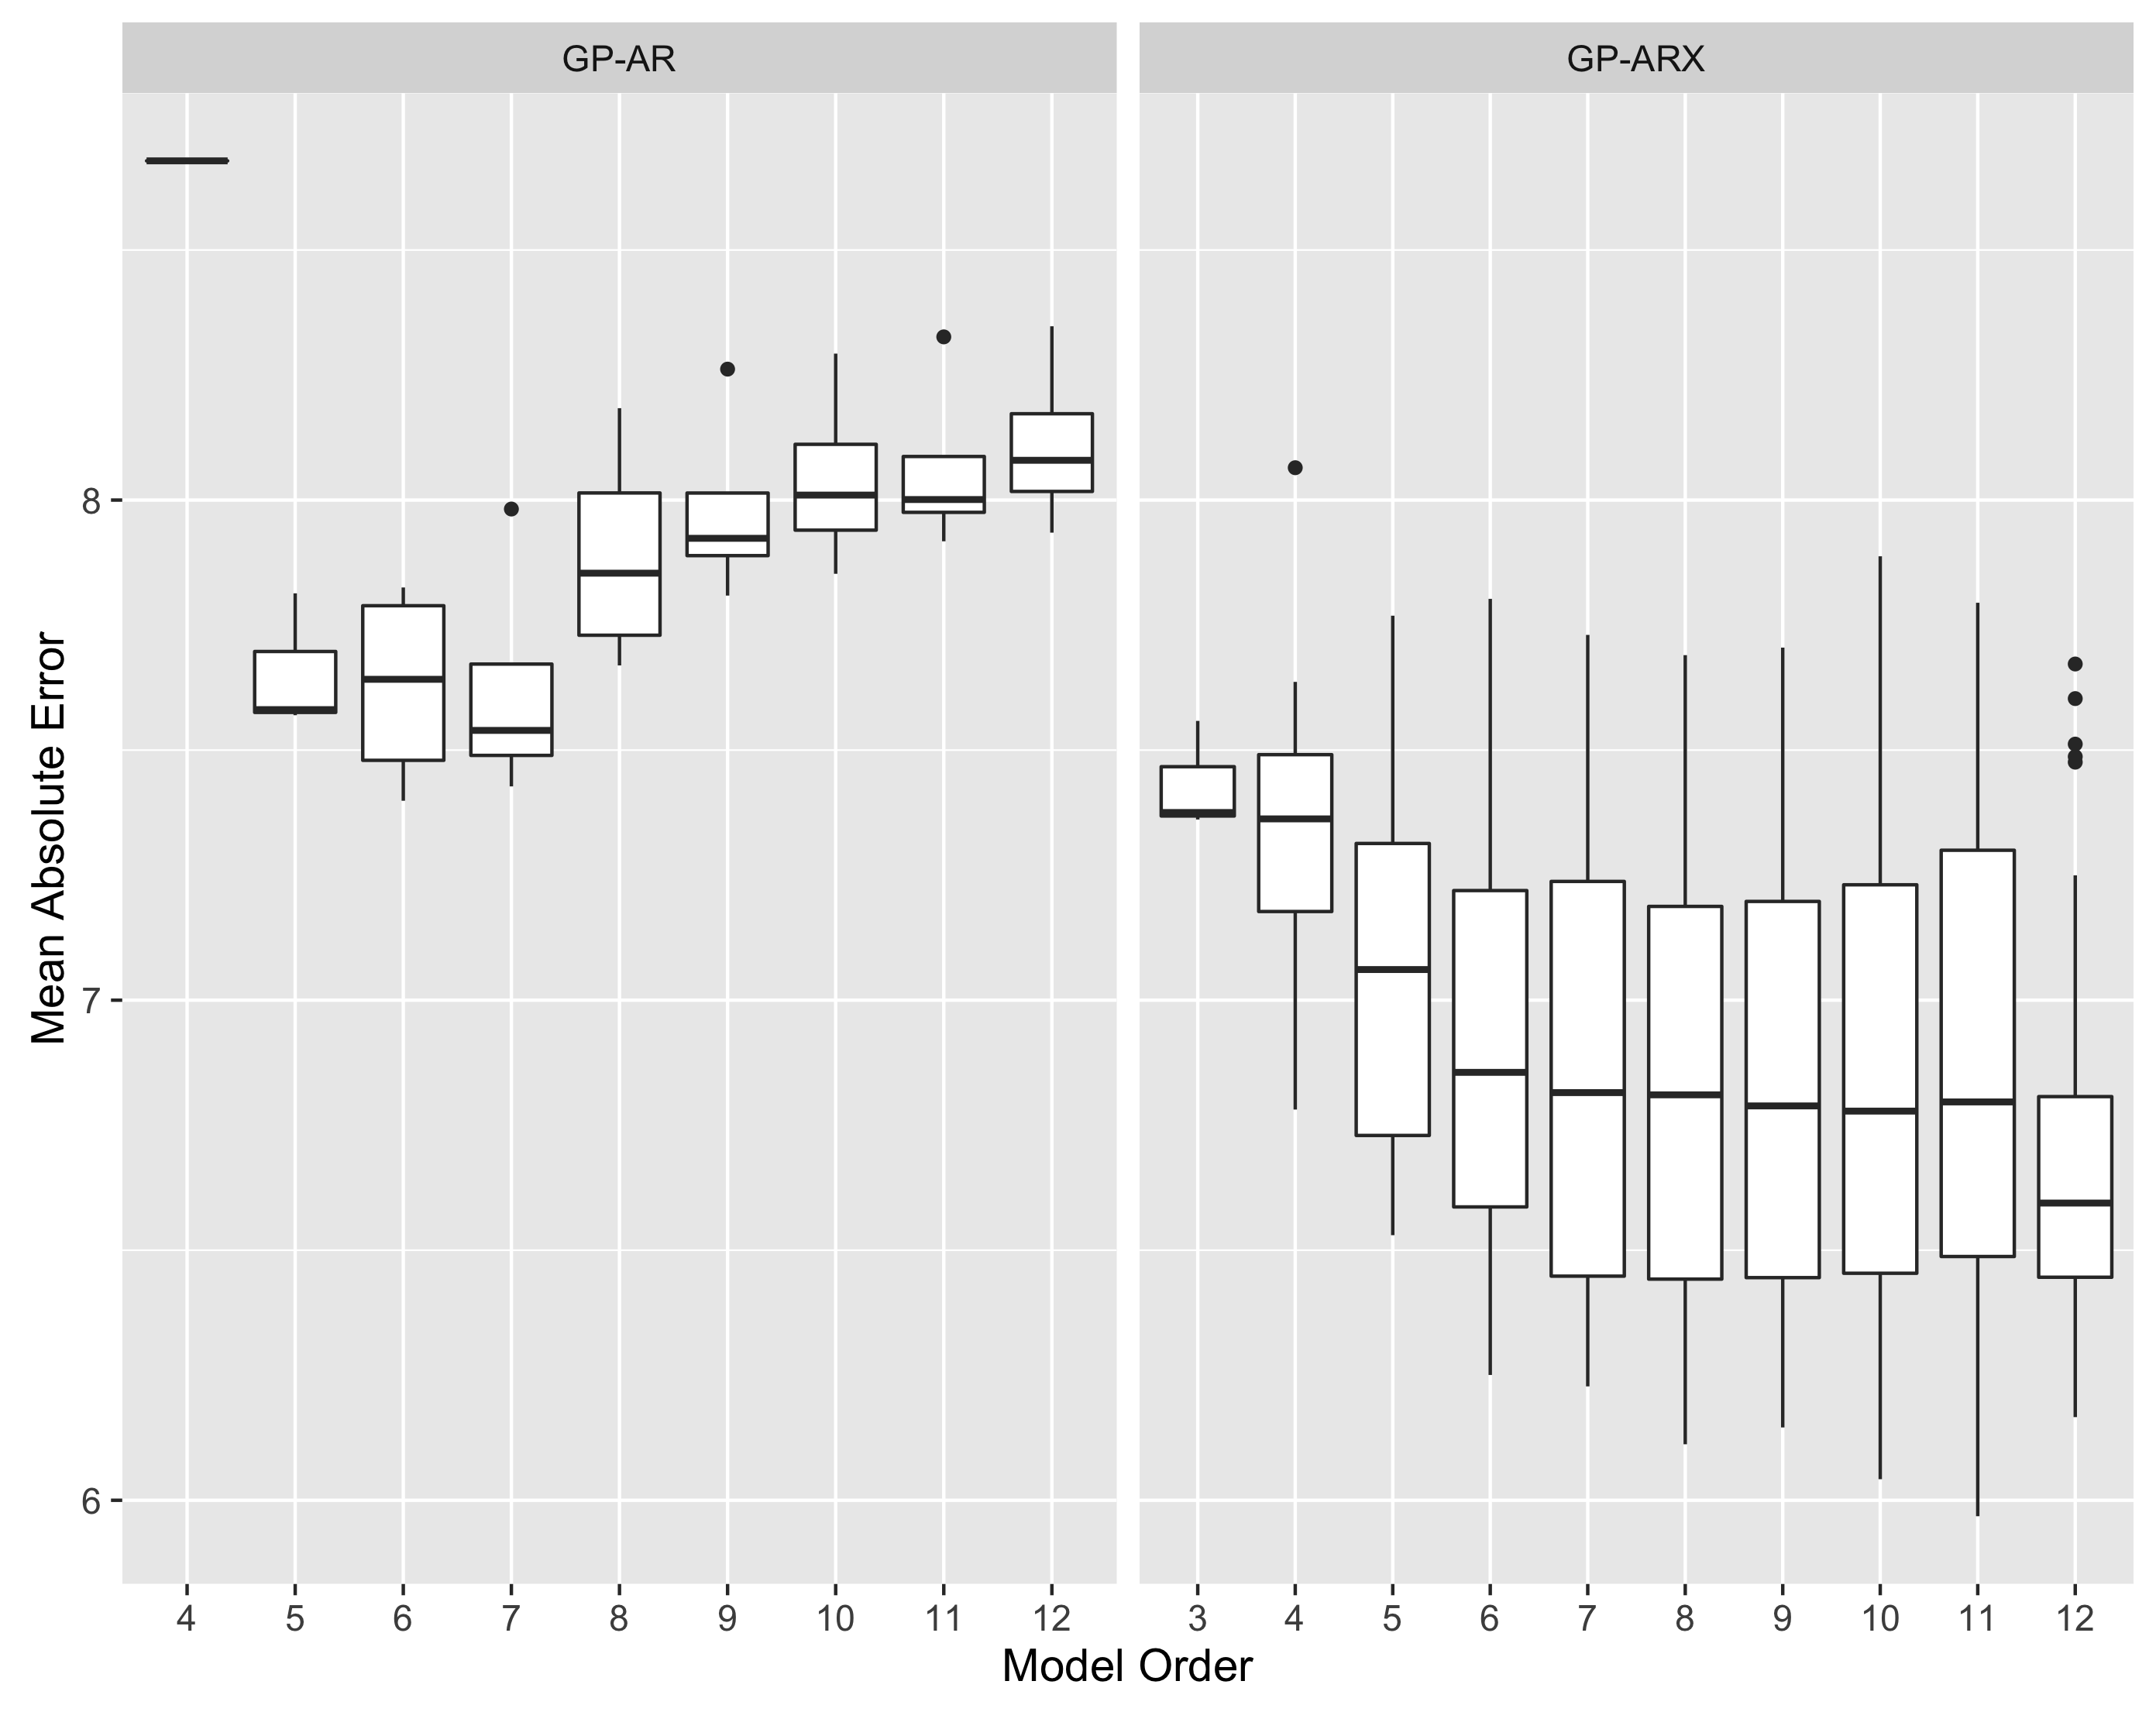
\includegraphics[width=\textwidth]{Compare-mae.png}
    \caption{Mean Absolute Error on validation set storms vs model order for GP-AR and GP-ARX. \\ \textbf{Key}: Rectangle borders represent the first and third quartiles, with a horizontal line inside to indicate the median value, outlying points are shown as dots and whiskers indicate the smallest and largest non-outliers}
    \label{fig:CompareMae}
    \end{figure}
    
    \begin{figure}
    \noindent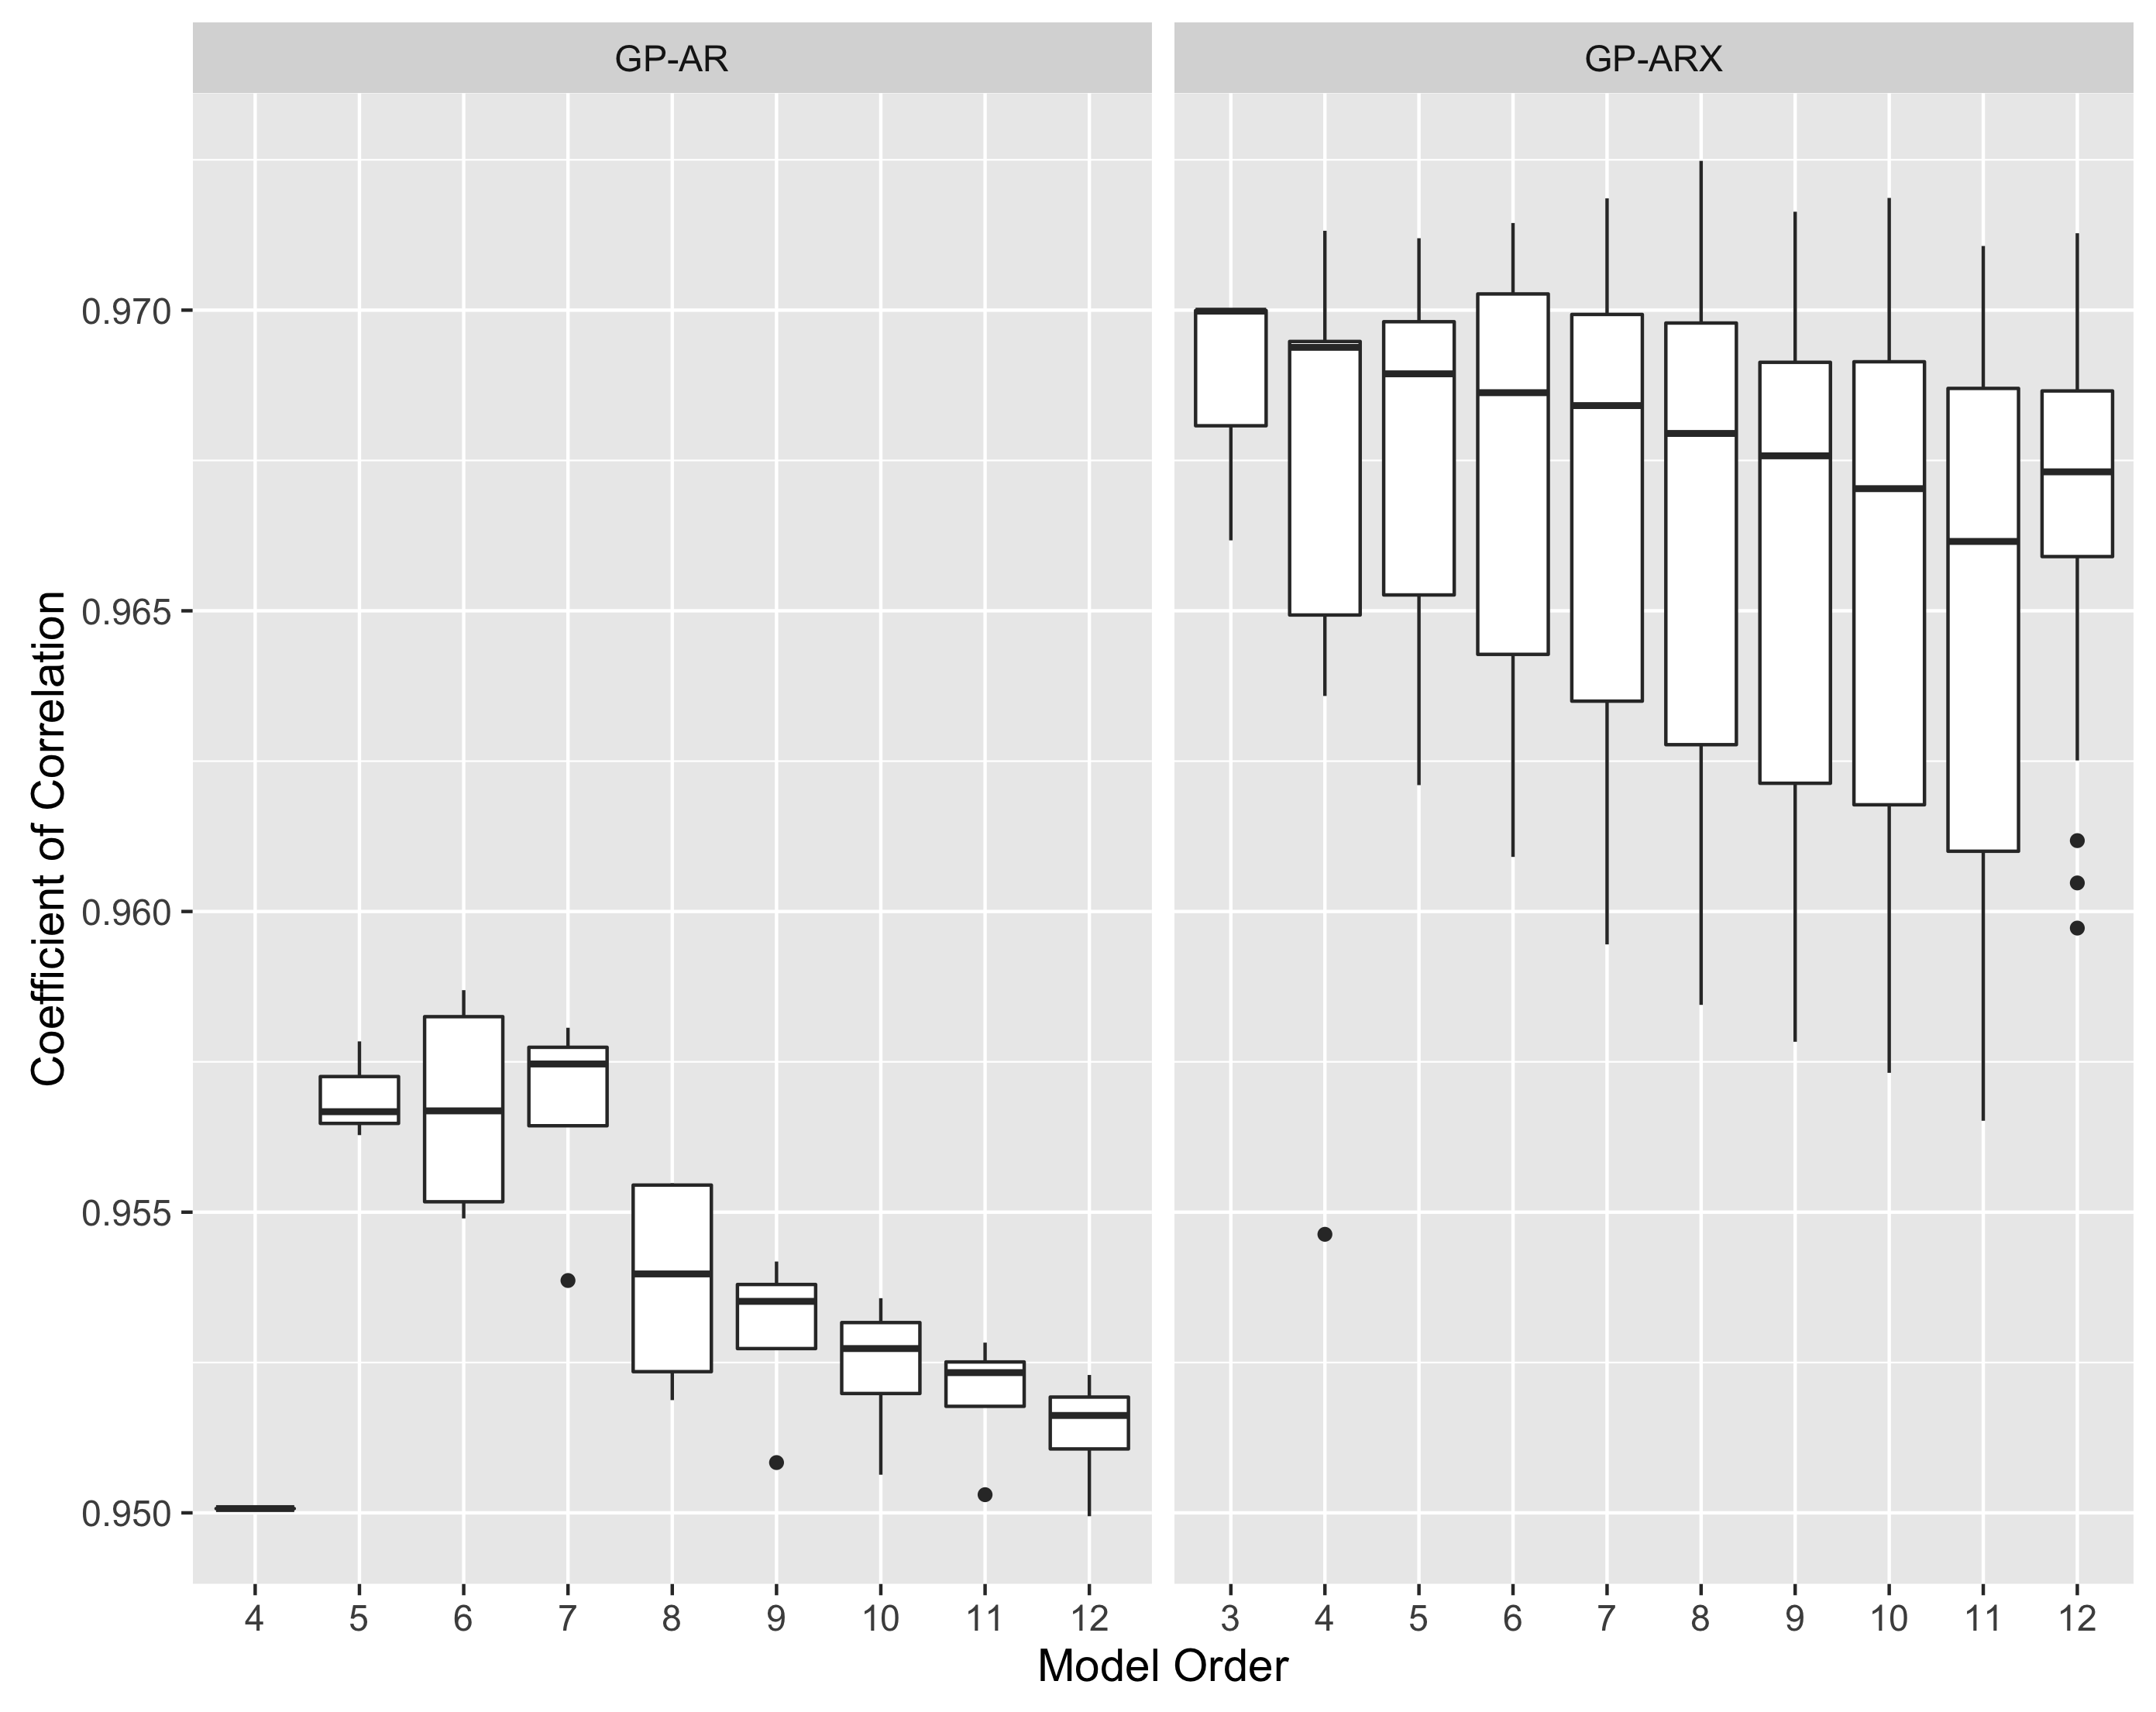
\includegraphics[width=\textwidth]{Compare-cc.png}
    \caption{Coefficient of Correlation on validation set storms vs model order for GP-AR and GP-ARX \\ \textbf{Key}: Rectangle borders represent the first and third quartiles, with a horizontal line inside to indicate the median value, outlying points are shown as dots and whiskers indicate the smallest and largest non-outliers}
    \label{fig:CompareCC}
    \end{figure}
    
    
    \begin{figure}
    \noindent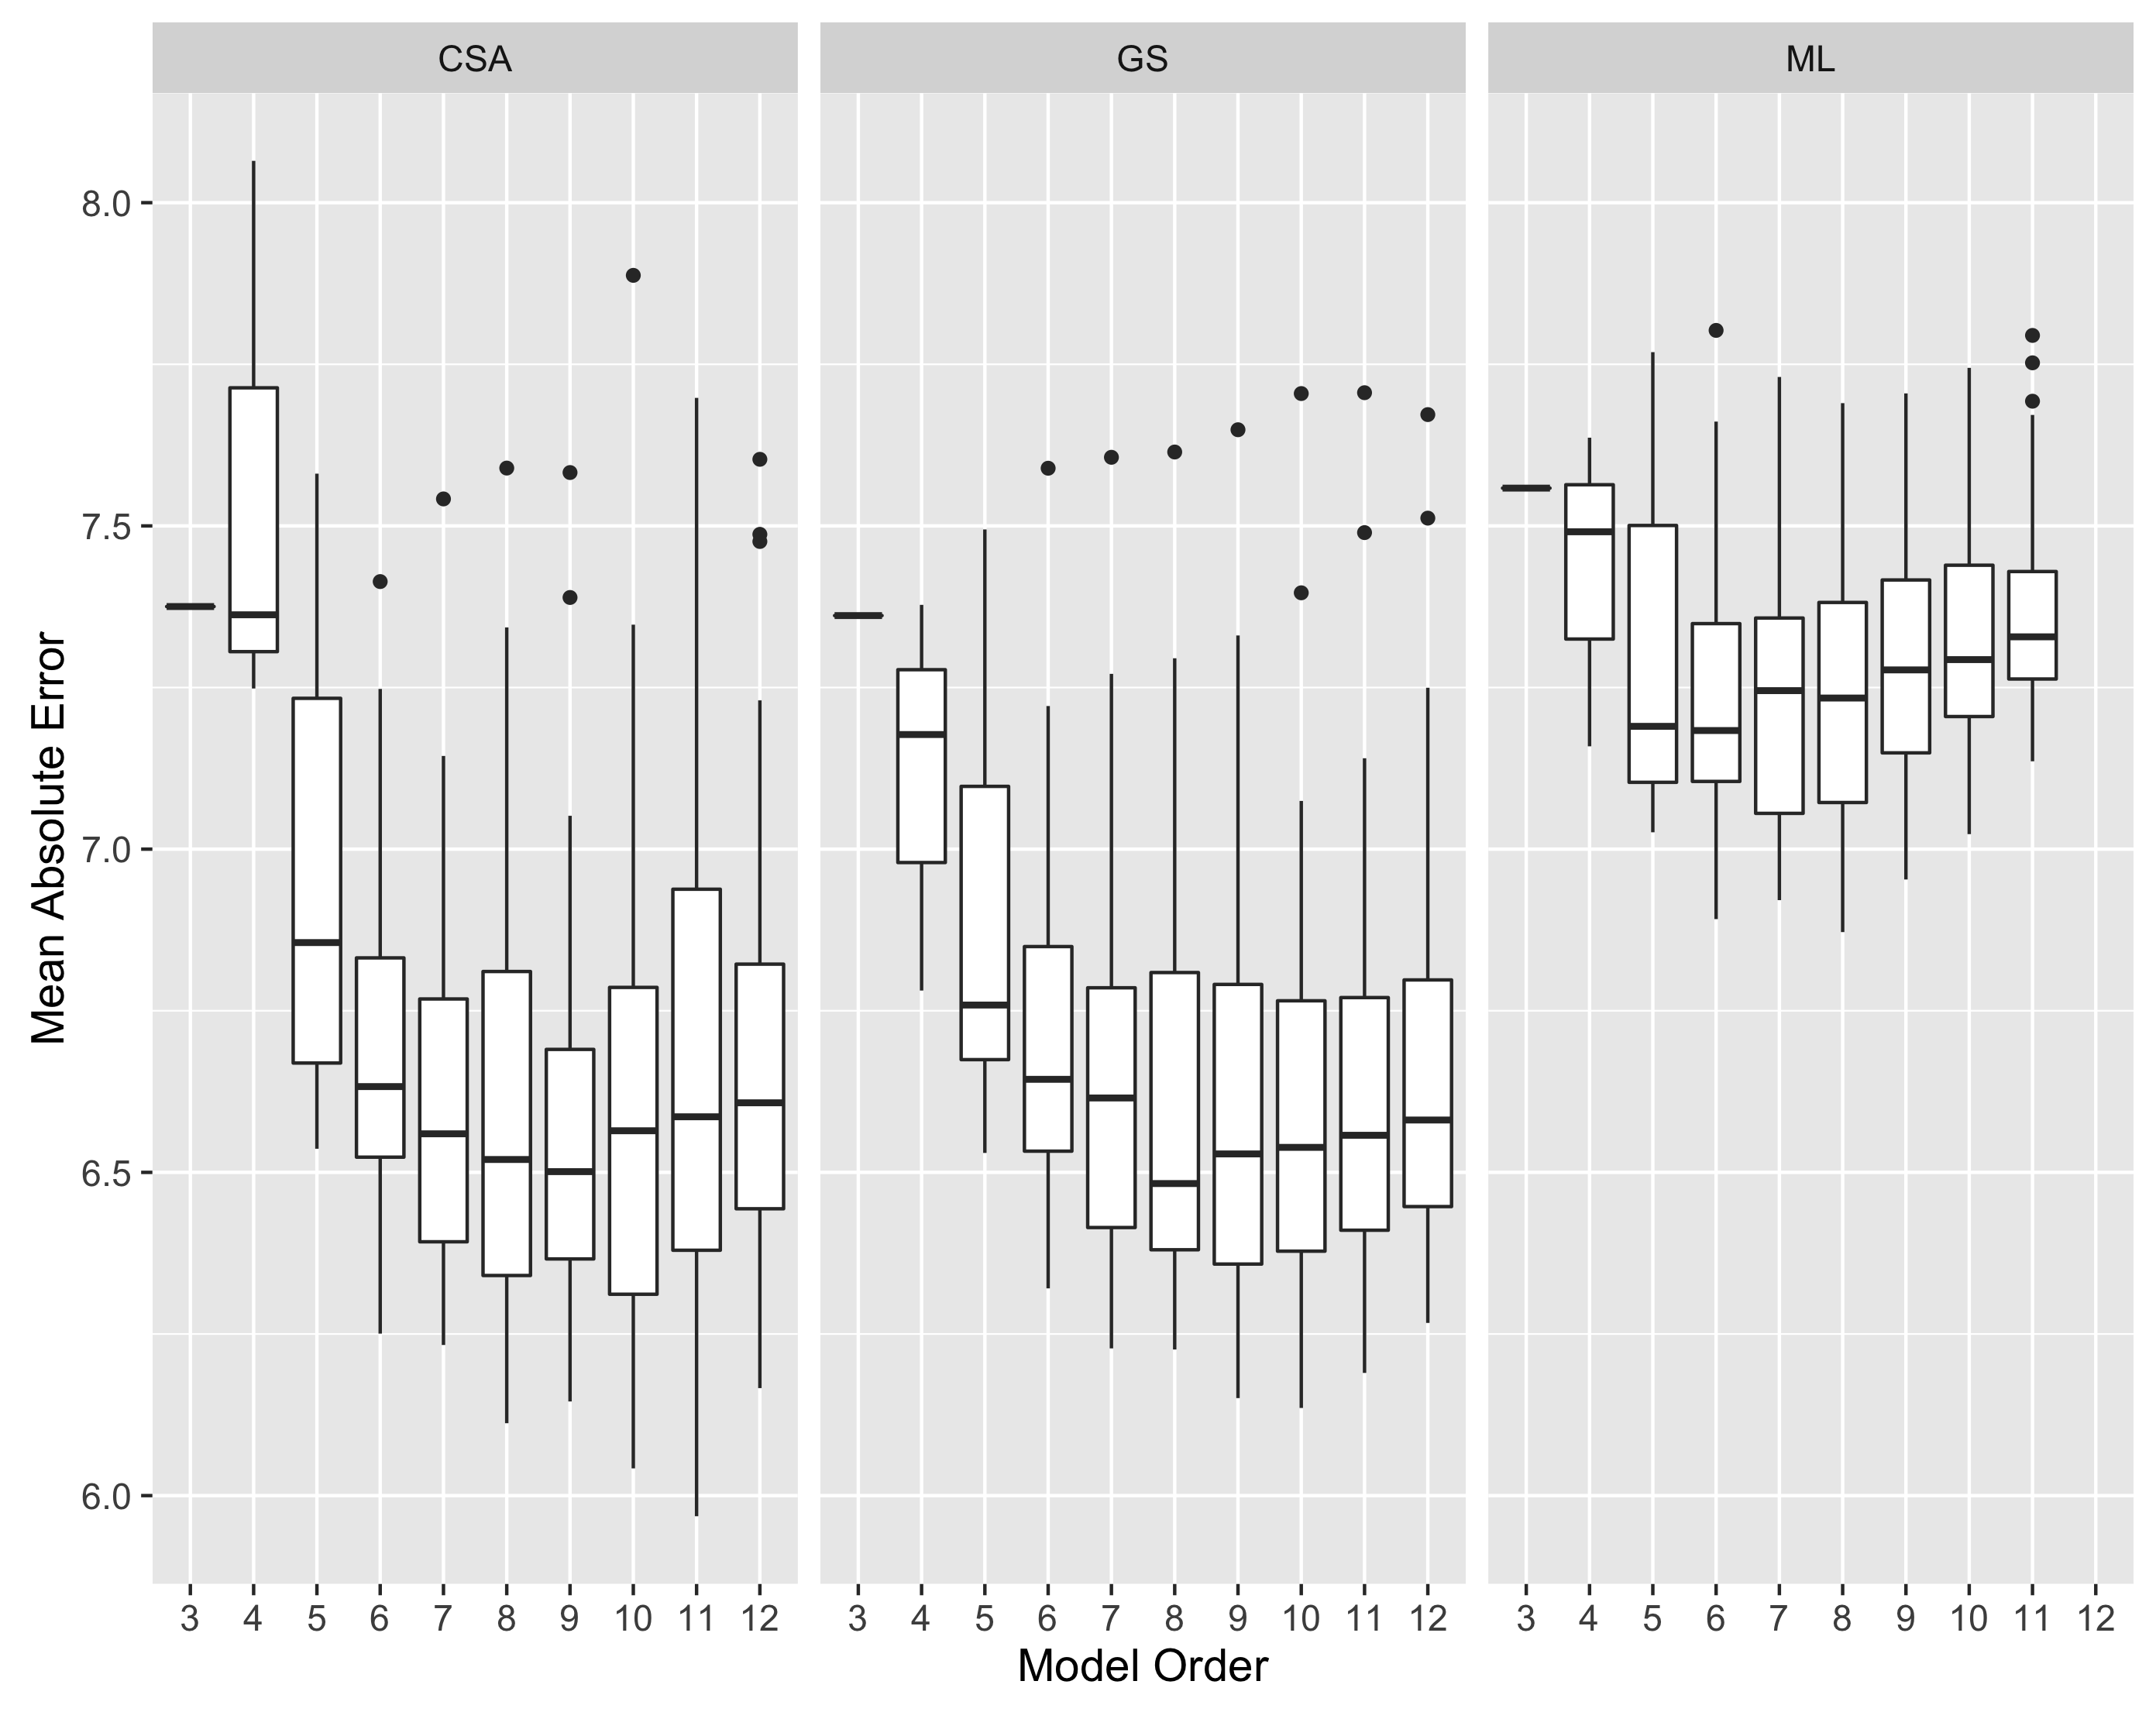
\includegraphics[width=\textwidth]{Compare-mae-arx.png}
    \caption{Mean Absolute Error on validation set storms vs model order for GP-AR and GP-ARX for \emph{CSA}, \emph{GS} and \emph{ML} model selection routines \\ \textbf{Key}: Rectangle borders represent the first and third quartiles, with a horizontal line inside to indicate the median value, outlying points are shown as dots and whiskers indicate the smallest and largest non-outliers}
    \label{fig:CompareMaeARX}
    \end{figure}
    
    \begin{figure}
    \noindent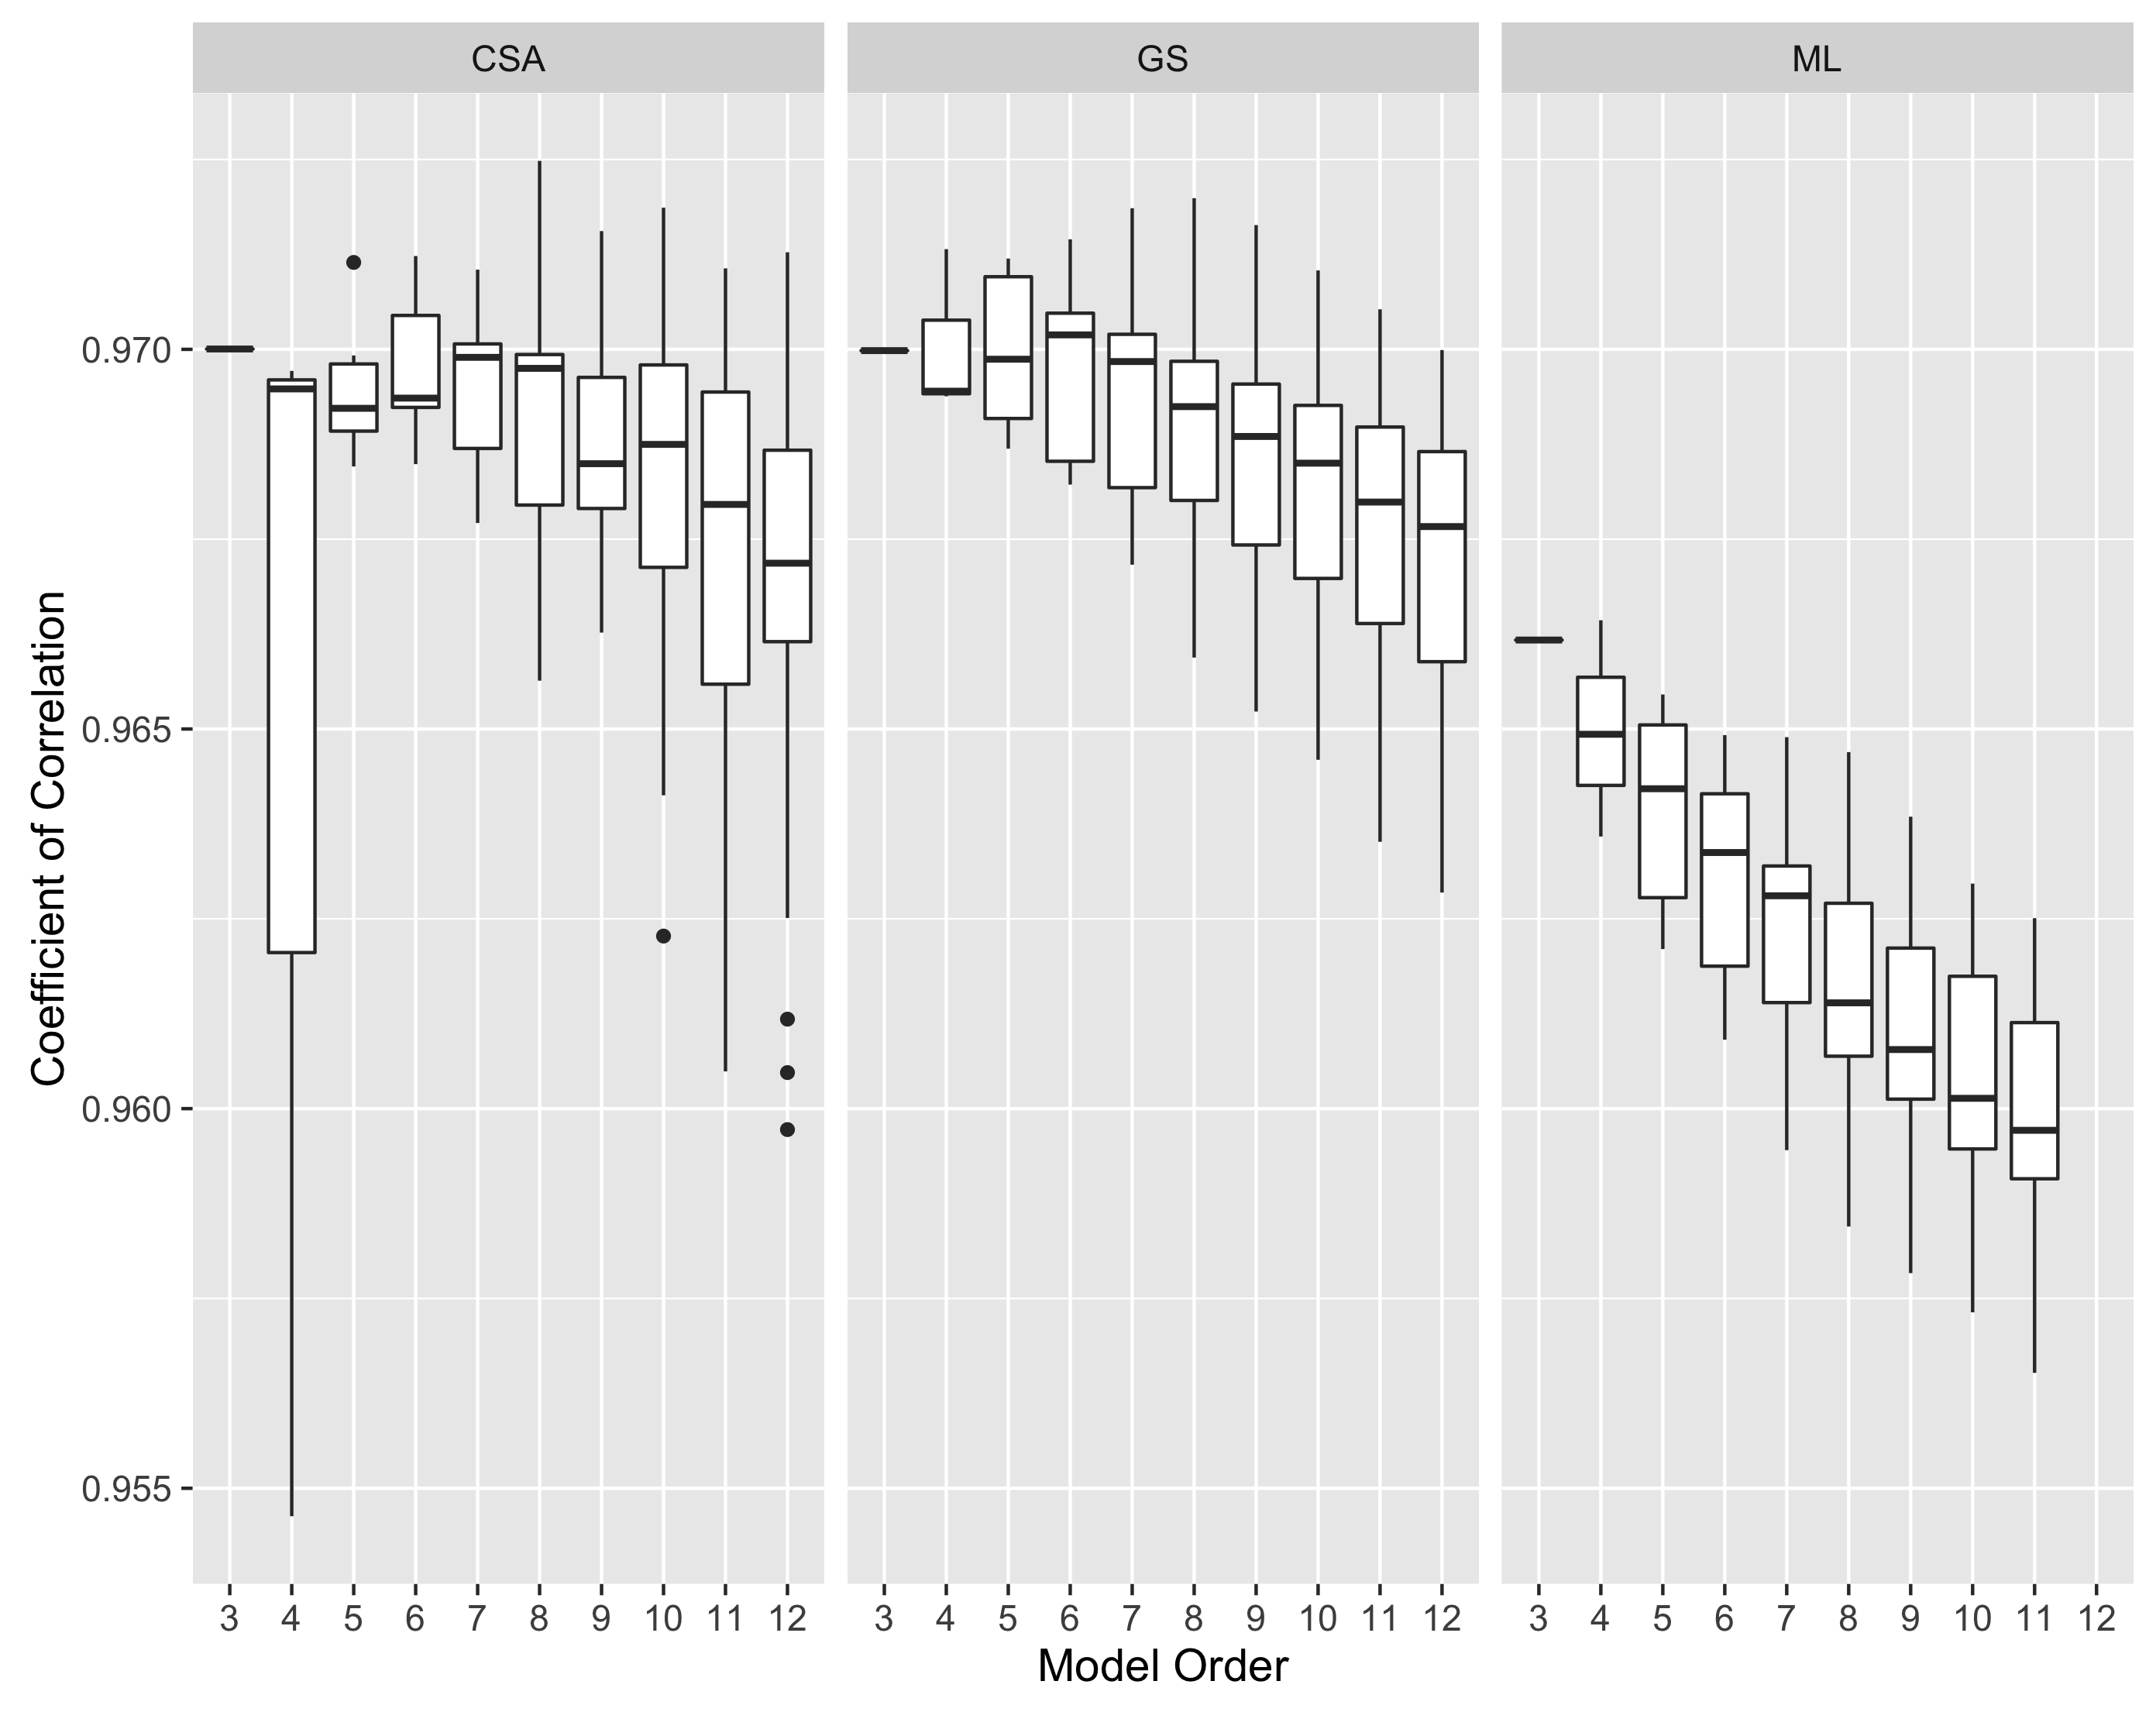
\includegraphics[width=\textwidth]{Compare-cc-arx.png}
    \caption{Coefficient of Correlation on validation set storms vs model order for GP-AR and GP-ARX for \emph{CSA}, \emph{GS} and \emph{ML} model selection routines \\ \textbf{Key}: Rectangle borders represent the first and third quartiles, with a horizontal line inside to indicate the median value, outlying points are shown as dots and whiskers indicate the smallest and largest non-outliers}
    \label{fig:CompareCCARX}
    \end{figure}
    
    
    \begin{figure}
    \noindent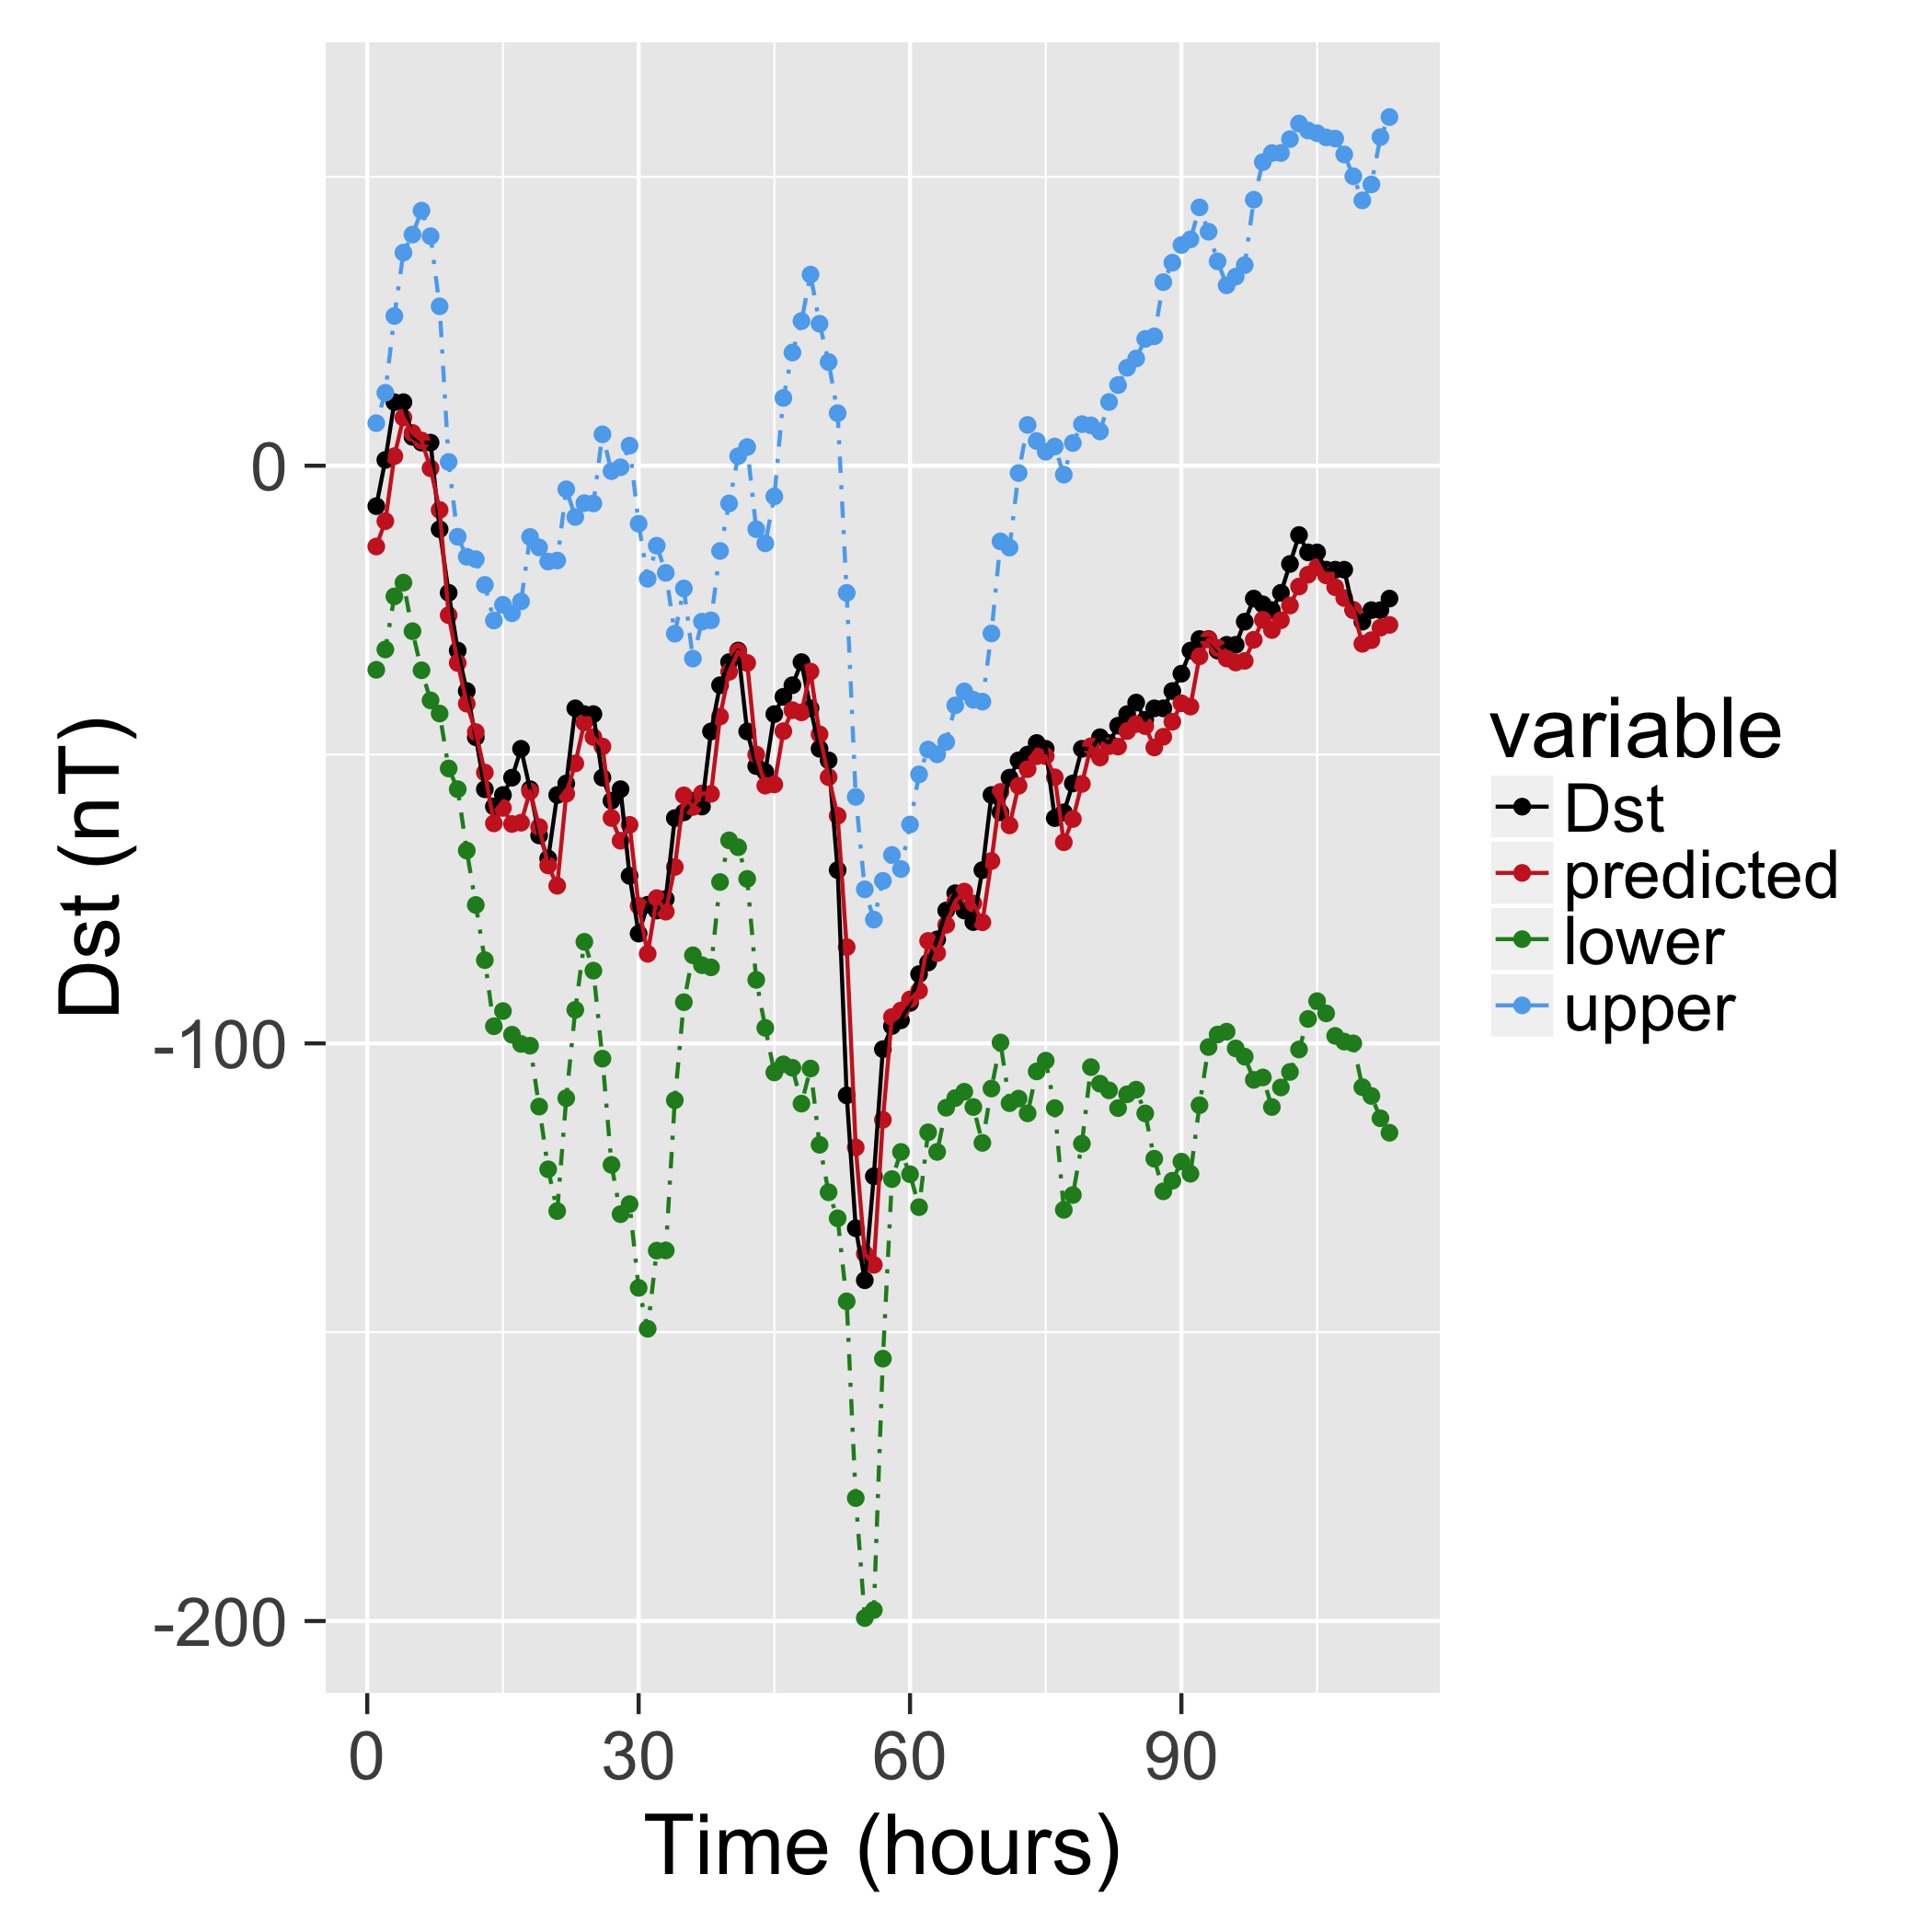
\includegraphics[width=\textwidth]{PredictionsModel1/PredErrBars_Storm43.png}
    \caption{OSA Predictions with $\pm \sigma$ error bars for event: 2003/06/17 to 2003/06/19}
    \label{fig:ComparePred1}
    \end{figure}
    
    
    \begin{figure}
    \noindent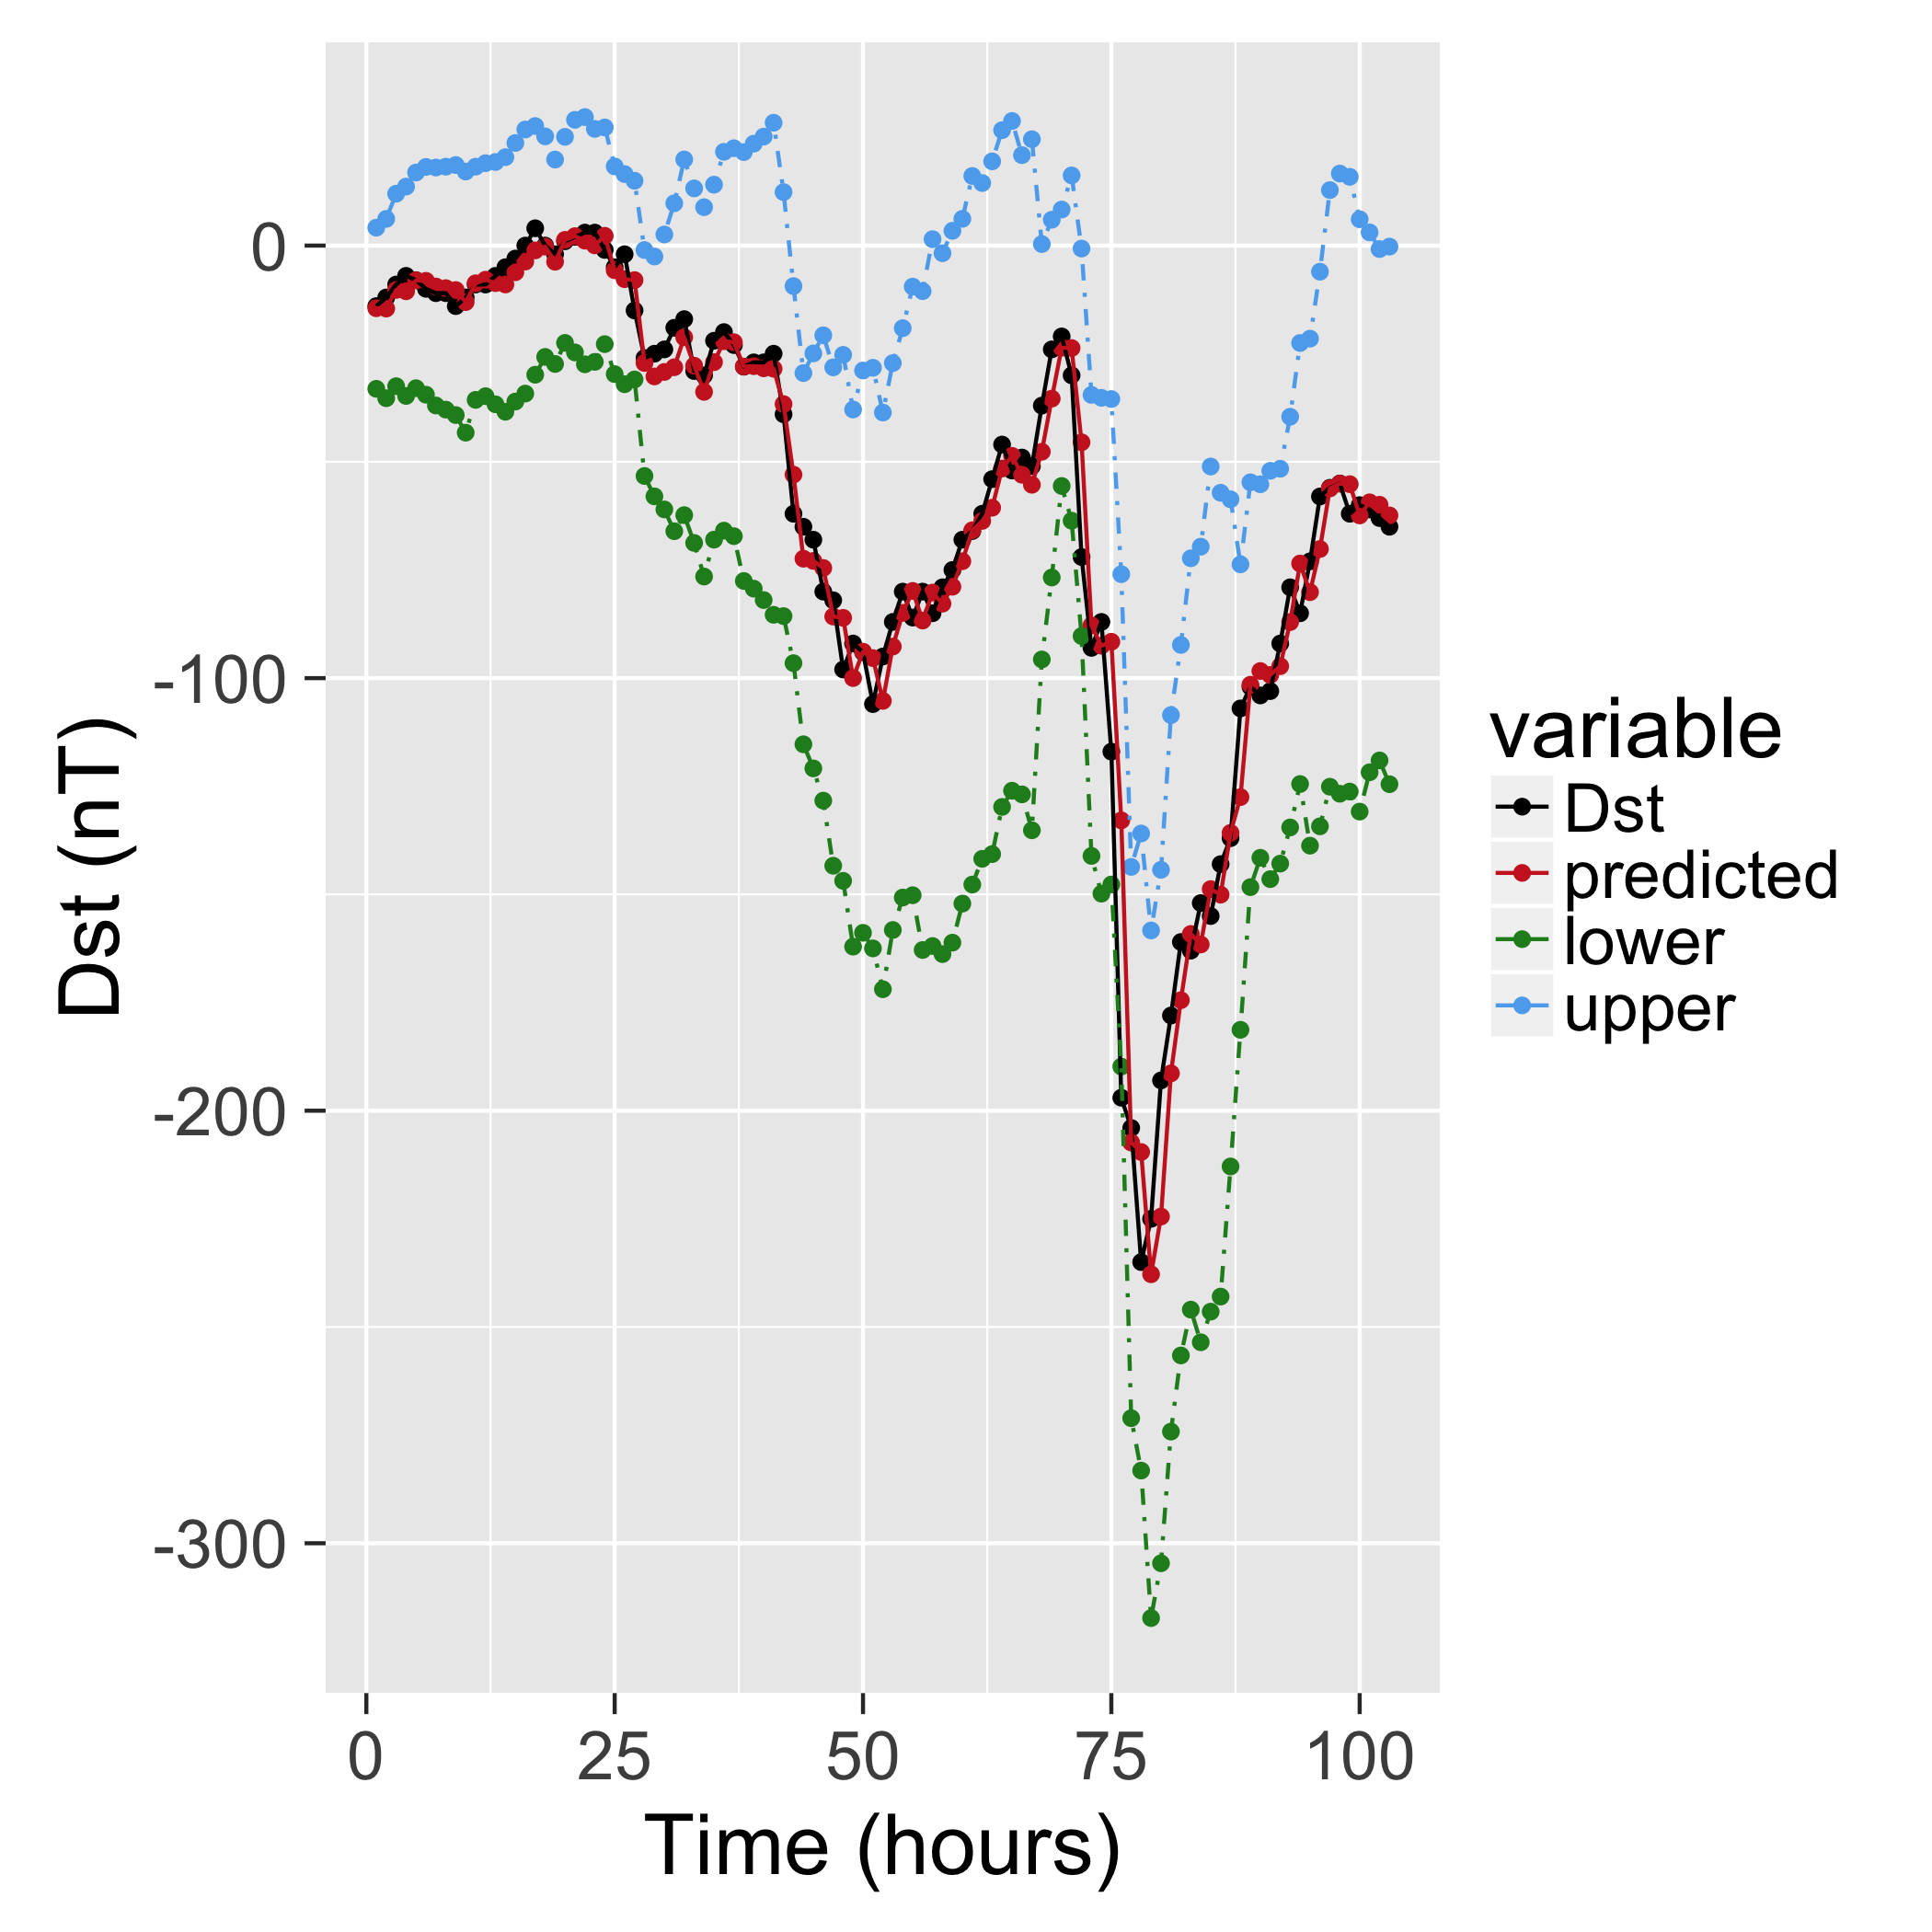
\includegraphics[width=\textwidth]{PredictionsModel1/PredErrBars_Storm16.png}
    \caption{OSA Predictions with $\pm \sigma$ error bars for event: 2012/03/08 to 2012/03/10}
    \label{fig:ComparePred2}
    \end{figure}
    
    \begin{figure}
    \noindent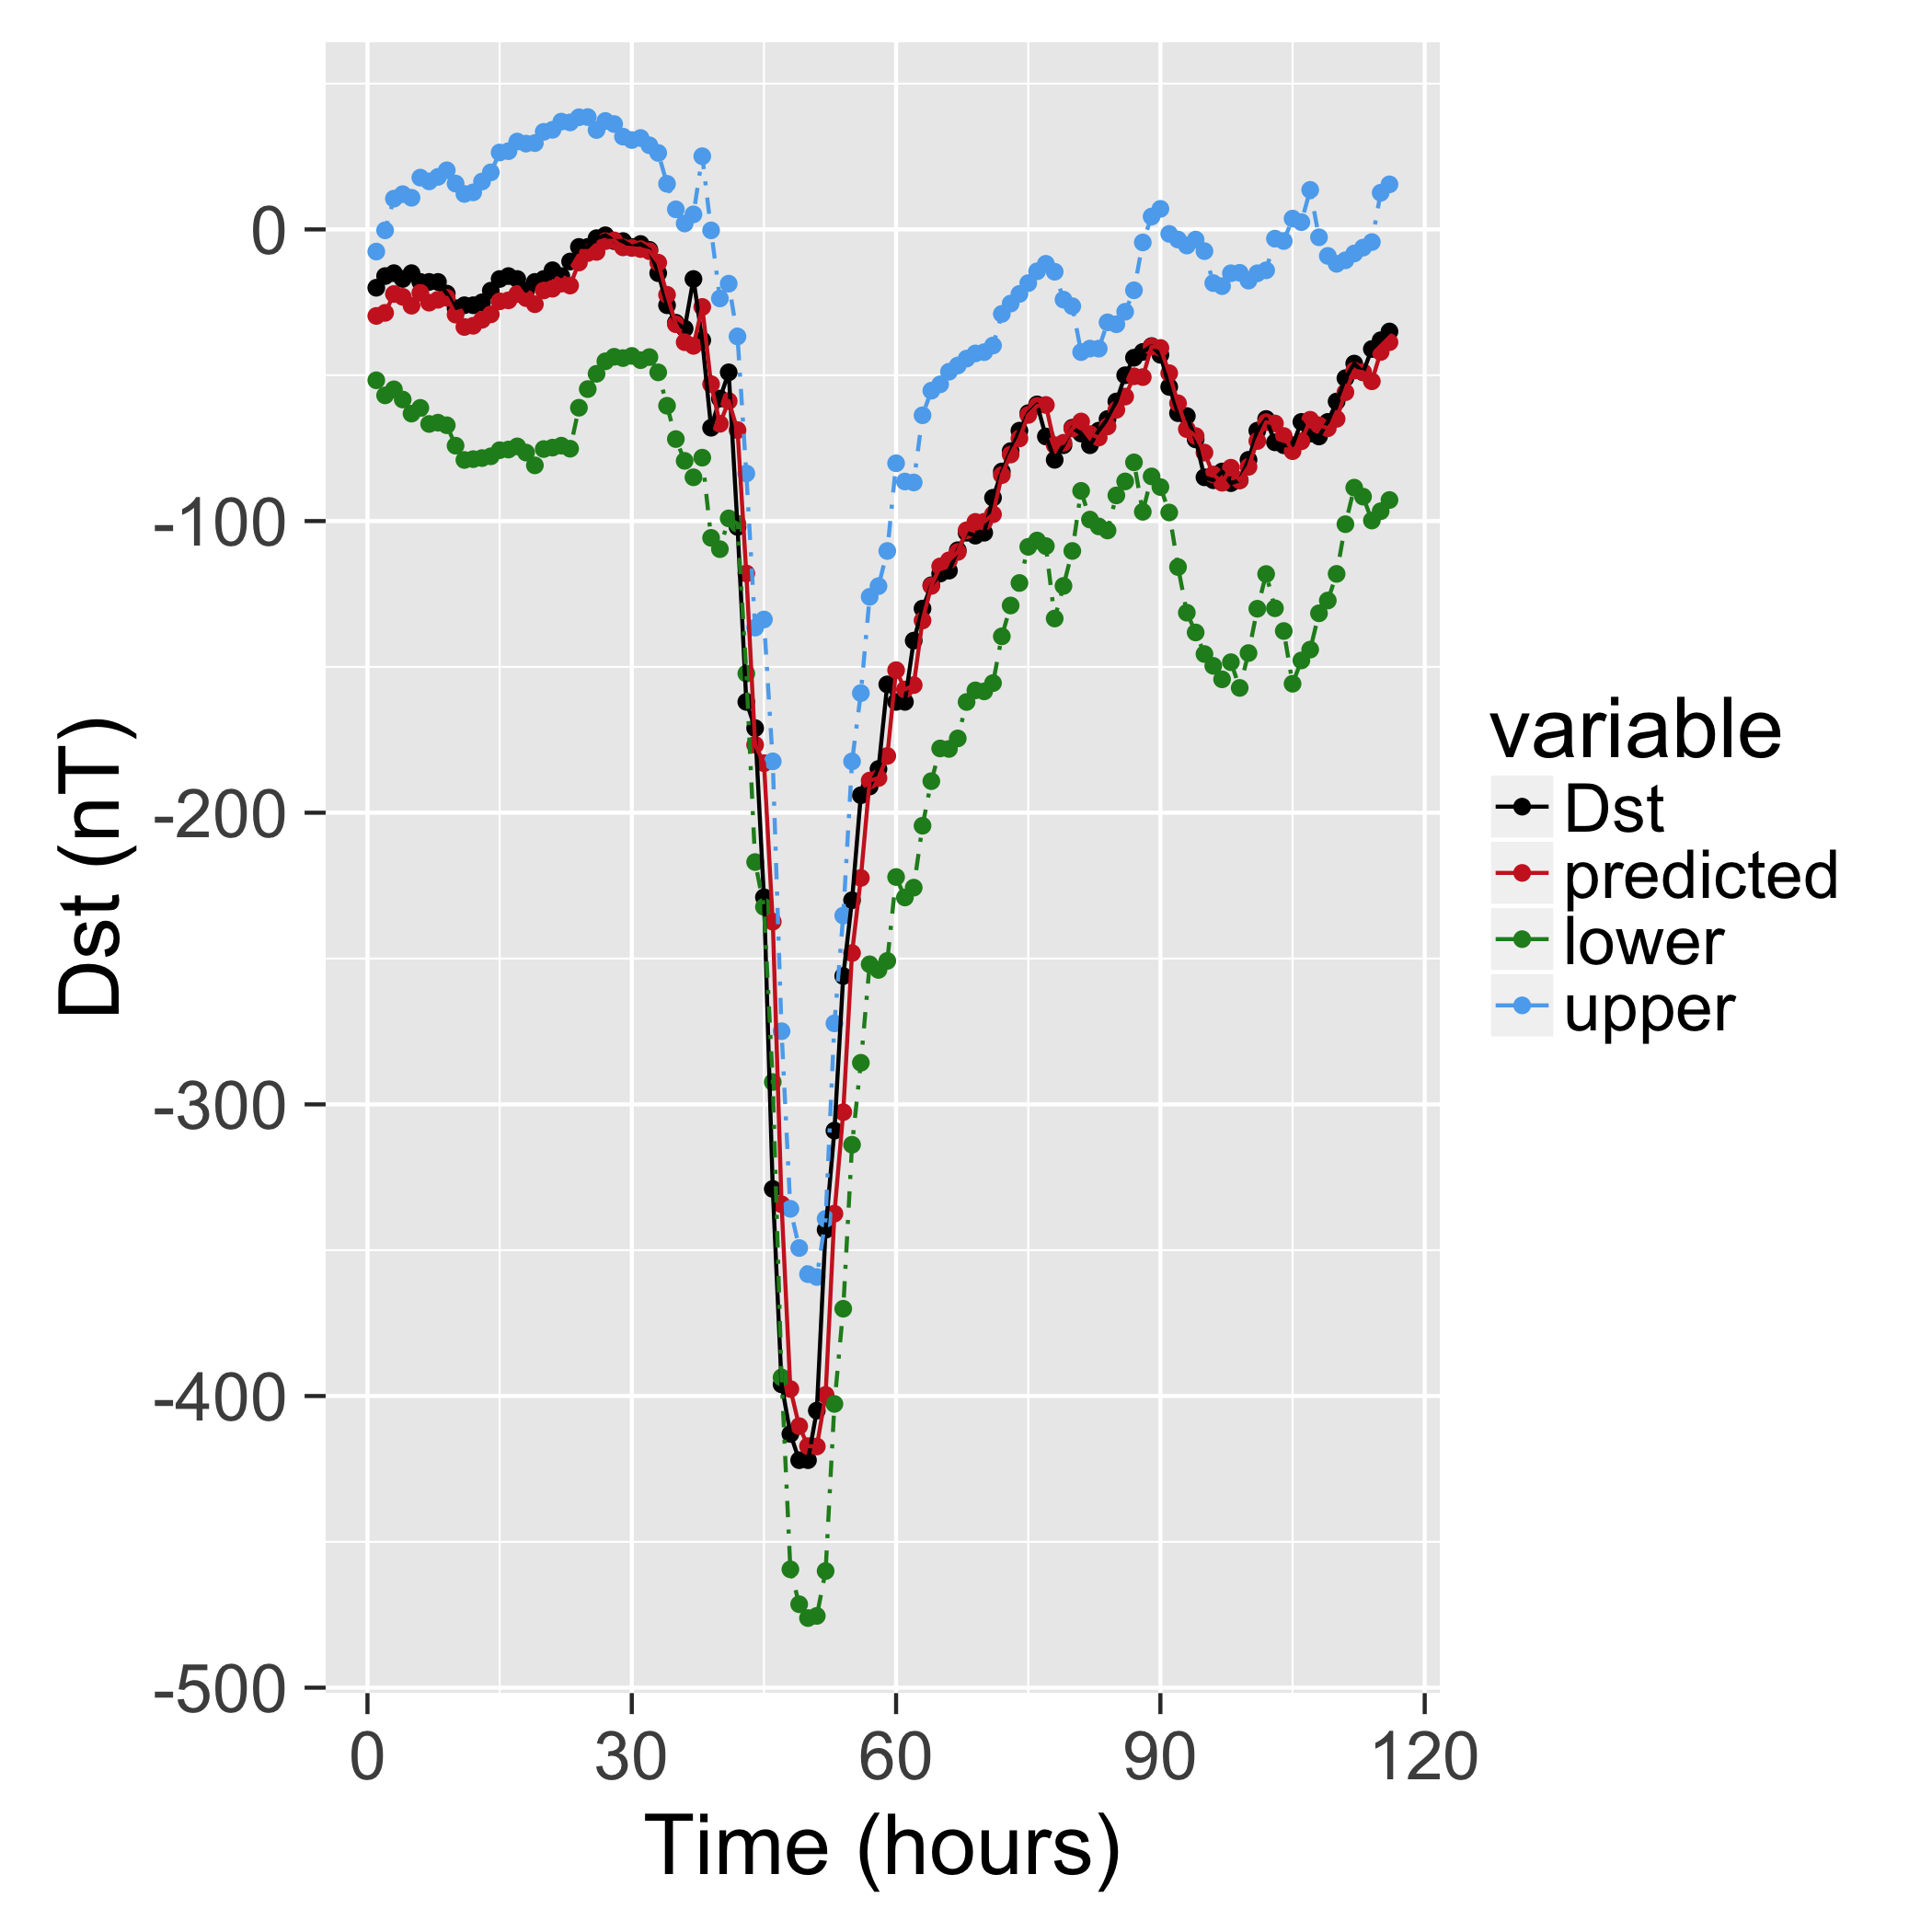
\includegraphics[width=\textwidth]{PredictionsModel1/PredErrBars_Storm46.png}
    \caption{OSA Predictions with $\pm \sigma$ error bars for event: 2003/11/20 to 2003/11/22}
    \label{fig:ComparePred3}
    \end{figure}
    
    
    %
    % ---------------
    % EXAMPLE TABLE
    %
    %\begin{table}
    %\caption{Time of the Transition Between Phase 1 and Phase 2\tablenotemark{a}}
    %\centering
    %\begin{tabular}{l c}
    %\hline
    % Run  & Time (min)  \\
    %\hline
    %  $l1$  & 260   \\
    %  $l2$  & 300   \\
    %  $l3$  & 340   \\
    %  $h1$  & 270   \\
    %  $h2$  & 250   \\
    %  $h3$  & 380   \\
    %  $r1$  & 370   \\
    %  $r2$  & 390   \\
    %\hline
    %\end{tabular}
    %\tablenotetext{a}{Footnote text here.}
    %\end{table}
    
    \begin{table}[h]
    \caption{Popular Kernel functions used in GPR models}
    \centering
    \begin{tabular}{l c c}
    \hline
     Name  & Expression & Hyperparameters  \\
    \hline
      Radial Basis Function (RBF)  & $\frac{1}{2} exp(-||\mathbf{x} - \mathbf{y}||^2/l^2)$  & $l \in \mathbb{R}$   \\
      
      Polynomial  & $(\mathbf{x}^\intercal \mathbf{y} + b)^d$ & $b \in \mathbb{R}, d \in \mathbb{N}$   \\
      
      Laplacian  & $exp(-||\mathbf{x} - \mathbf{y}||_{1}/\theta)$  & $\theta \in \mathbb{R}^+$  \\
      
      Student's T  & $1/(1 + ||\mathbf{x} - \mathbf{y}||_{2}^d)$ & $d \in \mathbb{R}^{+}$\\
      
      Maximum Likelihood Perceptron  & $sin^{-1}(\frac{w\mathbf{x}^\intercal \mathbf{y} + b}{\sqrt{w\mathbf{x}^\intercal \mathbf{x} + b + 1} \sqrt{w\mathbf{y}^\intercal \mathbf{y} + b + 1}})$ & $w, b \in \mathbb{R}^{+}$\\
    \hline
    \end{tabular}
    \label{table:kernel}
    \end{table}
    
    \begin{table}[h]
    \centering
    \caption{Settings of model selection procedures}
    \begin{tabular}{l c c c}
    \hline
    Procedure & Grid Size & Step & Max Iterations \\
    \hline
    Grid Search & 10 & 0.2 & NA \\
    Coupled Simulated Annealing & 4 & 0.2 & 30 \\
    Maximum likelihood & NA & 0.2 & 150\\
    \end{tabular}
    \label{table:modelselection}
    \end{table}
    
    
    \begin{table}[h]
    \centering
    \caption{Evaluation results for models on storm events listed in table \ref{table:teststorms}}
    \label{table:results}
    \begin{tabular}{l c c c}
    \hline
    Model & Mean Absolute Error & Root Mean Square Error & Coefficient of Correlation\\ \hline
    GP-ARX & 7.219 & 11.88 & 0.972\\
    GP-AR & 8.37 & 14.04 & 0.963\\
    Persistence & 9.182 & 14.94 & 0.957\\
    \end{tabular}
    \end{table}
    
    \begin{table}[h]
    \centering
    \caption{Storm events used for model selection of GP-AR and GP-ARX}
    \label{table:validationstorms}
    \begin{tabular}{llllll}
    \hline
    Event Id & Start Date & Start Hour & End Date & End Hour & min. Dst \\ \hline
    1 & 1995/03/26 & 05:00 & 1995/03/26 & 23:00 & $−107$ \\
    2 & 1995/04/07 & 13:00 & 1995/04/09 & 09:00 & $−149$ \\
    3 & 1995/09/27 & 01:00 & 1995/09/28 & 04:00 & $−108$ \\
    4 & 1995/10/18 & 13:00 & 1995/10/19 & 14:00 & $−127$ \\
    5 & 1996/10/22 & 22:00 & 1996/10/23 & 11:00 & $−105$ \\
    6 & 1997/04/21 & 10:00 & 1997/04/22 & 09:00 & $−107$ \\
    7 & 1997/05/15 & 03:00 & 1997/05/16 & 00:00 & $−115$ \\
    8 & 1997/10/10 & 18:00 & 1997/10/11 & 19:00 & $−130$ \\
    9 & 1997/11/07 & 00:00 & 1997/11/07 & 18:00 & $−110$ \\
    10 & 1997/11/22 & 21:00 & 1997/11/24 & 04:00 & $−108$ \\
    11 & 2005/06/12 & 17:00 & 2005/06/13 & 19:00 & $−106$ \\
    12 & 2005/08/31 & 12:00 & 2005/09/01 & 12:00 & $−122$ \\
    13 & 2006/12/14 & 21:00 & 2006/12/16 & 03:00 & $−162$ \\
    14 & 2011/09/26 & 14:00 & 2011/09/27 & 12:00 & $−101$ \\
    15 & 2011/10/24 & 20:00 & 2011/10/25 & 14:00 & $−132$ \\
    16 & 2012/03/08 & 12:00 & 2012/03/10 & 16:00 & $−131$ \\
    17 & 2012/04/23 & 11:00 & 2012/04/24 & 13:00 & $−108$ \\
    18 & 2012/07/15 & 01:00 & 2012/07/16 & 23:00 & $−127$ \\
    19 & 2012/09/30 & 13:00 & 2012/10/01 & 18:00 & $−119$ \\
    20 & 2012/10/08 & 02:00 & 2012/10/09 & 17:00 & $−105$ \\
    21 & 2012/11/13 & 18:00 & 2012/11/14 & 18:00 & $−108$ \\
    22 & 2013/03/17 & 07:00 & 2013/03/18 & 10:00 & $−132$ \\
    23 & 2013/05/31 & 18:00 & 2013/06/01 & 20:00 & $−119$ \\
    24 & 2014/02/18 & 15:00 & 2014/02/19 & 16:00 & $−112$
    \end{tabular}
    \end{table}
    
    

    \begin{table}[h]
    \fontsize{8}{9.6}\selectfont
    \centering
    \caption{Storm events used to evaluate GP-AR and GP-ARX models}
    \label{table:teststorms}
    \begin{tabular}{cccccc}
    \hline
    Event Id & Start Date & Start Time & End Date & End Time & min. Dst \\ \hline
    1 & 1998/02/17 & 12:00 & 1998/02/18 & 10:00 & -100 \\
    2 & 1998/03/10 & 11:00 & 1998/03/11 & 18:00 & -116 \\
    3 & 1998/05/04 & 02:00 & 1998/05/05 & 02:00 & -205 \\
    4 & 1998/08/26 & 10:00 & 1998/08/29 & 07:00 & -155 \\
    5 & 1998/09/25 & 01:00 & 1998/09/26 & 00:00 & -207 \\
    6 & 1998/10/19 & 05:00 & 1998/10/20 & 08:00 & -112 \\
    7 & 1998/11/09 & 03:00 & 1998/11/10 & 16:00 & -142 \\
    8 & 1998/11/13 & 00:00 & 1998/11/15 & 04:00 & -131 \\
    9 & 1999/01/13 & 16:00 & 1999/01/14 & 20:00 & -112 \\
    10 & 1999/02/18 & 03:00 & 1999/02/19 & 21:00 & -123 \\
    11 & 1999/09/22 & 20:00 & 1999/09/23 & 23:00 & -173 \\
    12 & 1999/10/22 & 00:00 & 1999/10/23 & 14:00 & -237 \\
    13 & 2000/02/12 & 05:00 & 2000/02/13 & 15:00 & -133 \\
    14 & 2000/04/06 & 17:00 & 2000/04/08 & 09:00 & -288 \\
    15 & 2000/05/24 & 01:00 & 2000/05/25 & 20:00 & -147 \\
    16 & 2000/08/10 & 20:00 & 2000/08/11 & 18:00 & -230 \\
    17 & 2000/08/12 & 02:00 & 2000/08/13 & 17:00 & -235 \\
    18 & 2000/10/13 & 02:00 & 2000/10/14 & 23:00 & -107 \\
    19 & 2000/10/28 & 20:00 & 2000/10/29 & 20:00 & -127 \\
    20 & 2000/11/06 & 13:00 & 2000/11/07 & 18:00 & -159 \\
    21 & 2000/11/28 & 18:00 & 2000/11/29 & 23:00 & -119 \\
    22 & 2001/03/19 & 15:00 & 2001/03/21 & 23:00 & -149 \\
    23 & 2001/03/31 & 04:00 & 2001/04/01 & 21:00 & -387 \\
    24 & 2001/04/11 & 16:00 & 2001/04/13 & 07:00 & -271 \\
    25 & 2001/04/18 & 01:00 & 2001/04/18 & 13:00 & -114 \\
    26 & 2001/04/22 & 02:00 & 2001/04/23 & 15:00 & -102 \\
    27 & 2001/08/17 & 16:00 & 2001/08/18 & 16:00 & -105 \\
    28 & 2001/09/30 & 23:00 & 2001/10/02 & 00:00 & -148 \\
    29 & 2001/10/21 & 17:00 & 2001/10/24 & 11:00 & -187 \\
    30 & 2001/10/28 & 03:00 & 2001/10/29 & 22:00 & -157 \\
    31 & 2002/03/23 & 14:00 & 2002/03/25 & 05:00 & -100 \\
    32 & 2002/04/17 & 11:00 & 2002/04/19 & 02:00 & -127 \\
    33 & 2002/04/19 & 09:00 & 2002/04/21 & 06:00 & -149 \\
    34 & 2002/05/11 & 10:00 & 2002/05/12 & 16:00 & -110 \\
    35 & 2002/05/23 & 12:00 & 2002/05/24 & 23:00 & -109 \\
    36 & 2002/08/01 & 23:00 & 2002/08/02 & 09:00 & -102 \\
    37 & 2002/09/04 & 01:00 & 2002/09/05 & 00:00 & -109 \\
    38 & 2002/09/07 & 14:00 & 2002/09/08 & 20:00 & -181 \\
    39 & 2002/10/01 & 06:00 & 2002/10/03 & 08:00 & -176 \\
    40 & 2002/10/03 & 10:00 & 2002/10/04 & 18:00 & -146 \\
    41 & 2002/11/20 & 16:00 & 2002/11/22 & 06:00 & -128 \\
    42 & 2003/05/29 & 20:00 & 2003/05/30 & 10:00 & -144 \\
    43 & 2003/06/17 & 19:00 & 2003/06/19 & 03:00 & -141 \\
    44 & 2003/07/11 & 15:00 & 2003/07/12 & 16:00 & -105 \\
    45 & 2003/08/17 & 18:00 & 2003/08/19 & 11:00 & -148 \\
    46 & 2003/11/20 & 12:00 & 2003/11/22 & 00:00 & -422 \\
    47 & 2004/01/22 & 03:00 & 2004/01/24 & 00:00 & -149 \\
    48 & 2004/02/11 & 10:00 & 2004/02/12 & 00:00 & -105 \\
    49 & 2004/04/03 & 14:00 & 2004/04/04 & 08:00 & -112 \\
    50 & 2004/07/22 & 20:00 & 2004/07/23 & 20:00 & -101 \\
    51 & 2004/07/24 & 21:00 & 2004/07/26 & 17:00 & -148 \\
    52 & 2004/07/26 & 22:00 & 2004/07/30 & 05:00 & -197 \\
    53 & 2004/08/30 & 05:00 & 2004/08/31 & 21:00 & -126 \\
    54 & 2004/11/07 & 21:00 & 2004/11/08 & 21:00 & -373 \\
    55 & 2004/11/09 & 11:00 & 2004/11/11 & 09:00 & -289 \\
    56 & 2004/11/11 & 22:00 & 2004/11/13 & 13:00 & -109 \\
    57 & 2005/01/21 & 18:00 & 2005/01/23 & 05:00 & -105 \\
    58 & 2005/05/07 & 20:00 & 2005/05/09 & 10:00 & -127 \\
    59 & 2005/05/29 & 22:00 & 2005/05/31 & 08:00 & -138 \\
    60 & 2005/06/12 & 17:00 & 2005/06/13 & 19:00 & -106 \\
    61 & 2005/08/31 & 12:00 & 2005/09/01 & 12:00 & -131 \\
    62 & 2006/04/13 & 20:00 & 2006/04/14 & 23:00 & -111 \\
    63 & 2006/12/14 & 21:00 & 2006/12/16 & 03:00 & -147 \\ \hline
    \end{tabular}%
    \end{table}
    

\bibliographystyle{plain}
\bibliography{references-ch-dst}


\clearemptydoublepage

\chapter{Second Real Chapter}\label{chapter:second_real_chapter}
And the second real chapter.

\clearemptydoublepage

\chapter{Conclusions}\label{chapter:conclusions}
\chapter{Concluding Remarks}\label{chapter:conclusions}

This thesis represents an exploration of the possibilities for using machine learning techniques 
for advancing space weather research. The work presented here was classified into three principal 
research problems or themes as mentioned in \cref{chapter:Outline}. Below we give a quick summary 
of the main achievements of this thesis and avenues for further research.

\section{Discussion}

\subsection*{Geomagnetic Time Series Forecasting}

Using Gaussian process auto-regressive methods, it is possible to obtain accurate and reliable 
probabilistic forecasts for the $\mathrm{Dst}$ index, up to five hours ahead. 

The GP-AR and GP-ARX models give a general framework for modeling non-linear dynamical systems and 
provide uncertainty estimates on their time evolution. Their main drawback is the $O(N^3)$ time 
complexity for performing inference which makes applications on large data sets challenging. By 
using neural network based models as mean functions of GP models, one can create hybrid models 
which somewhat circumvent this drawbacks while retaining the probabilistic forecasting 
capabilities.

\subsection*{Radiation Belt Parameter Inference}

Using machine learning models as surrogates for quantities governed by physical laws, one can 
obtain models with some desirable properties: the ability synthesise observations and prior 
knowledge of physical dynamics into a coherent methodology for parameter inference and uncertainty 
quantification. 

When performing inference over the parameters of the radiation belt dynamics, one needs to take 
into account the sensitivity of the radiation belt model to its parameters. It is advisable to use 
domain knowledge and sensitivity analysis to constrain the numerical ranges of the parameter 
prior distributions as this aides identification and obtaining compact uncertainty estimates.

Casting the surrogate optimisation problem (\cref{eq:surrogate}) in its dual form enables the use 
of potentially infinite dimensional basis function expansions but it introduces the same 
computational challenges that come with Gaussian process inference. 

\subsection*{Solar Wind Prediction}

The effect of time lag relationships between interacting systems can impact the performance of 
predictive models which give forecasts for a fixed time lag. We proposed a principled approach for 
training predictive models on time series data sets which have non-stationary time lag dependencies.

The task of predicting near-Earth solar wind speed from heliospheric data is very challenging and 
requires astute application of all the tools at our disposal: 
\begin{enumerate*} 
    \item models of the heliospheric magnetic field,
    \item machine learning techniques, and 
    \item solar and near-Earth data. 
\end{enumerate*}


\section{Further Research}

Although the space weather problem is the central motivation for the work presented here, the 
techniques presented in this thesis are generally applicable in the modeling and forecasting of 
physical systems. Some possible questions for further research are listed below.

\begin{enumerate}
    \item With the existing state of the art, how far we extend the time horizon of geomagnetic 
          activity forecasts? What kind of data and methods will be important in making 
          ten-hour-ahead or twelve-hour-ahead forecasts of the $\mathrm{Dst}$ index?
    \item How do we extend the phase space density surrogate model to higher dimensional 
          radiation belt dynamics i.e. diffusion across all three adiabatic invariants?
          How do we deal with the computational challenges that arise from performing inference 
          over parameters of $3$-d diffusion models and large scale data sets? 
    \item When working in the context of PDE constrained inverse problems, how do we separate 
          uncertainties arising from parameter identifiability and forward model inadequacy? How do 
          we perform inference over the parameters of a non-linear PDE using machine learning based 
          surrogate models?
    \item How can we improve the accuracy of solar wind forecasts made by the \XX \ model? How can 
          we make the combination of the CSSS and \XX \ models into a real time solar wind 
          forecasting system? Is it beneficial to use a surrogate in place of the CSSS model to 
          compute the topology of the HMF? 
\end{enumerate}

All things considered, there are plenty of directions for further research into applications of 
machine learning methods in space weather and the physical sciences.


\clearemptydoublepage

%Choose a good bibliography style, plain would do often, but these might be nice too
%\bibliographystyle{these}
\bibliographystyle{plain}
\bibliography{references}

\clearemptydoublepage

\appendix
\addcontentsline{toc}{chapter}{Appendix}

\chapter{My First Appendix}
In this file (appendices/main.tex) you can add appendix chapters, just as you did in the thesis.tex file for the `normal' chapters.
You can also choose to include everything in this single file, whatever you prefer.

\end{document}
